\section{Синтез математической модели объекта управления}

\begin{figure}[H]
    \centering
    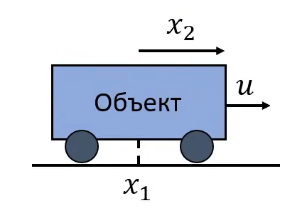
\includegraphics[width=0.5\linewidth]{figs/cart.png}
    \caption{Тележка}
    \label{fig:cart}
\end{figure}

Рассмотрим объект управления тележка, представленный на \autoref{fig:cart},
где $x_1$ --- положение тележки, $x_2$ --- скорость тележки, значит $\dot x_1=x_2$.
Управляем ускорением тележки $u$.
Синтезируем математическую модель тележки,
\begin{equation}
    \label{eq:sys}
    \begin{cases}
        \dot x=Ax+Bu+B_ww\\
        y=Cx+D_ww\\
    \end{cases},
\end{equation}
приняв за состояние
\begin{equation*}
    x(t)=\begin{bmatrix}
        x_1(t)\\
        x_2(t)
    \end{bmatrix},
\end{equation*}
в качестве невозмущенной компоненты выхода линейную координату
$y(t)=Cx(t)=x_1(t)$ и считая, что возмущение
\begin{equation*}
    w_\omega(t)=\begin{bmatrix}
        sin(\omega t)\\
        0
    \end{bmatrix}
\end{equation*}
посредством матрицы $B_w$
аддитивно с управлением действует на вектор состояния $x(t)$ и посредством матрицы $D_w$ 
влияет на выход. Матрицы $B_w$ и $D_w$ зададим следующими
\begin{equation*}
    B_w=\begin{bmatrix}
        1 & 0 \\
        1 & 0
    \end{bmatrix},\quad
    D_w=\begin{bmatrix}
        0 & 1
    \end{bmatrix},
\end{equation*}
чтобы $B_wD_w^T=0$ и $DD^T$ была обратима (ЕСЛИ КТО-ТО ДЕЛАЕТ РАБОТУ ПО ОБРАЗЦУ 
ЭТОЙ, ТО ВОЗМУЩЕНИЕ ДОЛЖНО БЫТЬ В СОСТОЯНИИ И ВЫХОДЕ, А НЕ КАК В МОЕЙ РАБОТЕ, 
ГДЕ ОНО ПРИСУТСТВУЕТ ТОЛЬКО В СОСТОЯНИИ). Остальные матрицы следующие:
\begin{equation*}
    A=\begin{bmatrix}
        0 & 1 \\
        0 & 0
    \end{bmatrix},\quad
    B=\begin{bmatrix}
        0 \\
        1
    \end{bmatrix},\quad
    C=\begin{bmatrix}
        1 & 0
    \end{bmatrix}.
\end{equation*}

Зададимся двумя вариантами регулируемого выхода
\begin{equation}
    z(t)=C_Zx+D_Zu.
\end{equation}
В первом варианте будем минимизировать координату тележки и управление, но 
координату предпочтительнее:
\begin{equation*}
    C_{Z1}=\begin{bmatrix}
        10 & 0 \\
        0 & 0
    \end{bmatrix},\quad
    D_{Z1}=\begin{bmatrix}
        0 \\
        1
    \end{bmatrix}.
\end{equation*}
Во втором варианте будем минимизировать координату тележки, скорость и упралвение, но 
скорость "сильнее" всего:
\begin{equation*}
    C_{Z2}=\begin{bmatrix}
        10 & 50 \\
        0 & 0
    \end{bmatrix},\quad
    D_{Z2}=\begin{bmatrix}
        0 \\
        1
    \end{bmatrix}.
\end{equation*}
Матрицы выбраны таким образом, что $C_Z^TD_Z=0$ и $D_Z^TD_Z$ обратима.

Для синтеза регуляторов потребуется, чтобы пара ($A,\ B$) была стабилизируемой и 
пара ($C_Z,\ A$) - наблюдаема. Проверим это:
\begin{equation*}
    U_{(A,\ B)}=\begin{bmatrix}
        0	&1\\
        1	&0
    \end{bmatrix},\quad
    V_{(C_{Z1},\ A)}=\begin{bmatrix}
        10	&0\\
        0&	0\\
        0	&10\\
        0	&0
    \end{bmatrix},\quad
    V_{(C_{Z2},\ A)}=\begin{bmatrix}
        10	&50\\
        0&	0\\
        0	&10\\
        0	&0
    \end{bmatrix}.
\end{equation*}
Как можно заметить, все матрицы имеют ранг 2, значит требуемые условия выполняются.
Для синтеза наблюдателей понадобится, чтобы пара ($C,\ A$) была
обнаруживаемой и пара ($A,\ B_w$) была управляемой. Проверим это:
\begin{equation*}
    V_{(C,\ A)}=\begin{bmatrix}
        1	&0\\
        0&	1
    \end{bmatrix},\quad
    U_{(A,\ B_w)}=\begin{bmatrix}
        1	&0&	1	&0\\
        1&0&	0	&0
    \end{bmatrix}.
\end{equation*}
Матрицы имеет ранг 2, значит требуемые условия выполняются.





\section{Синтез H2-регулятора по состоянию}

\subsection{Первый вариант регулируемого выхода}
\label{sec:regout1}

Синтезируем H2-регулятор вида $u=Kx$ по состоянию для $C_{Z1}$ и $D_{Z1}$ путем решения матричного
уравнения Риккати:
\begin{equation}
    \label{eq:ric1}
    A^TQ+QA+C_Z^TC_Z-QB(D_Z^TD_Z)^{-1}B^TQ=0,\quad K=-(D_Z^TD_Z)^{-1}B^TQ.
\end{equation}
Используя \texttt{icare} получим
\begin{equation*}
    K=\begin{bmatrix}
        -10.0000&-4.4721
    \end{bmatrix}.
\end{equation*}
Получим систему, где вход $w$ и выход $z$, просто подставив $u=Kx$ в \eqref{eq:sys}:
\begin{equation*}
    \begin{cases}
        \dot x=(A+BK)x+B_ww\\
        z=(C_Z+D_ZK)x.
    \end{cases}
\end{equation*}
Передаточная матрица замкнутой системы от внешнего возмущения $w$ к выходу $z$:
\begin{equation*}
    \underset{w\rightarrow z}{W}(s)=\begin{bmatrix}
        \dfrac{10s+54.72}{s^2+4.472s+10} & 0 \\[2ex]
        \dfrac{-14.47s-10}{s^2+4.472s+10} & 0
    \end{bmatrix}
\end{equation*}
График покомпонентных АЧХ $\underset{w\rightarrow z}{W}(s)$ представлен на \autoref{fig:1bodemag}.
\begin{figure}[H]
    \centering
    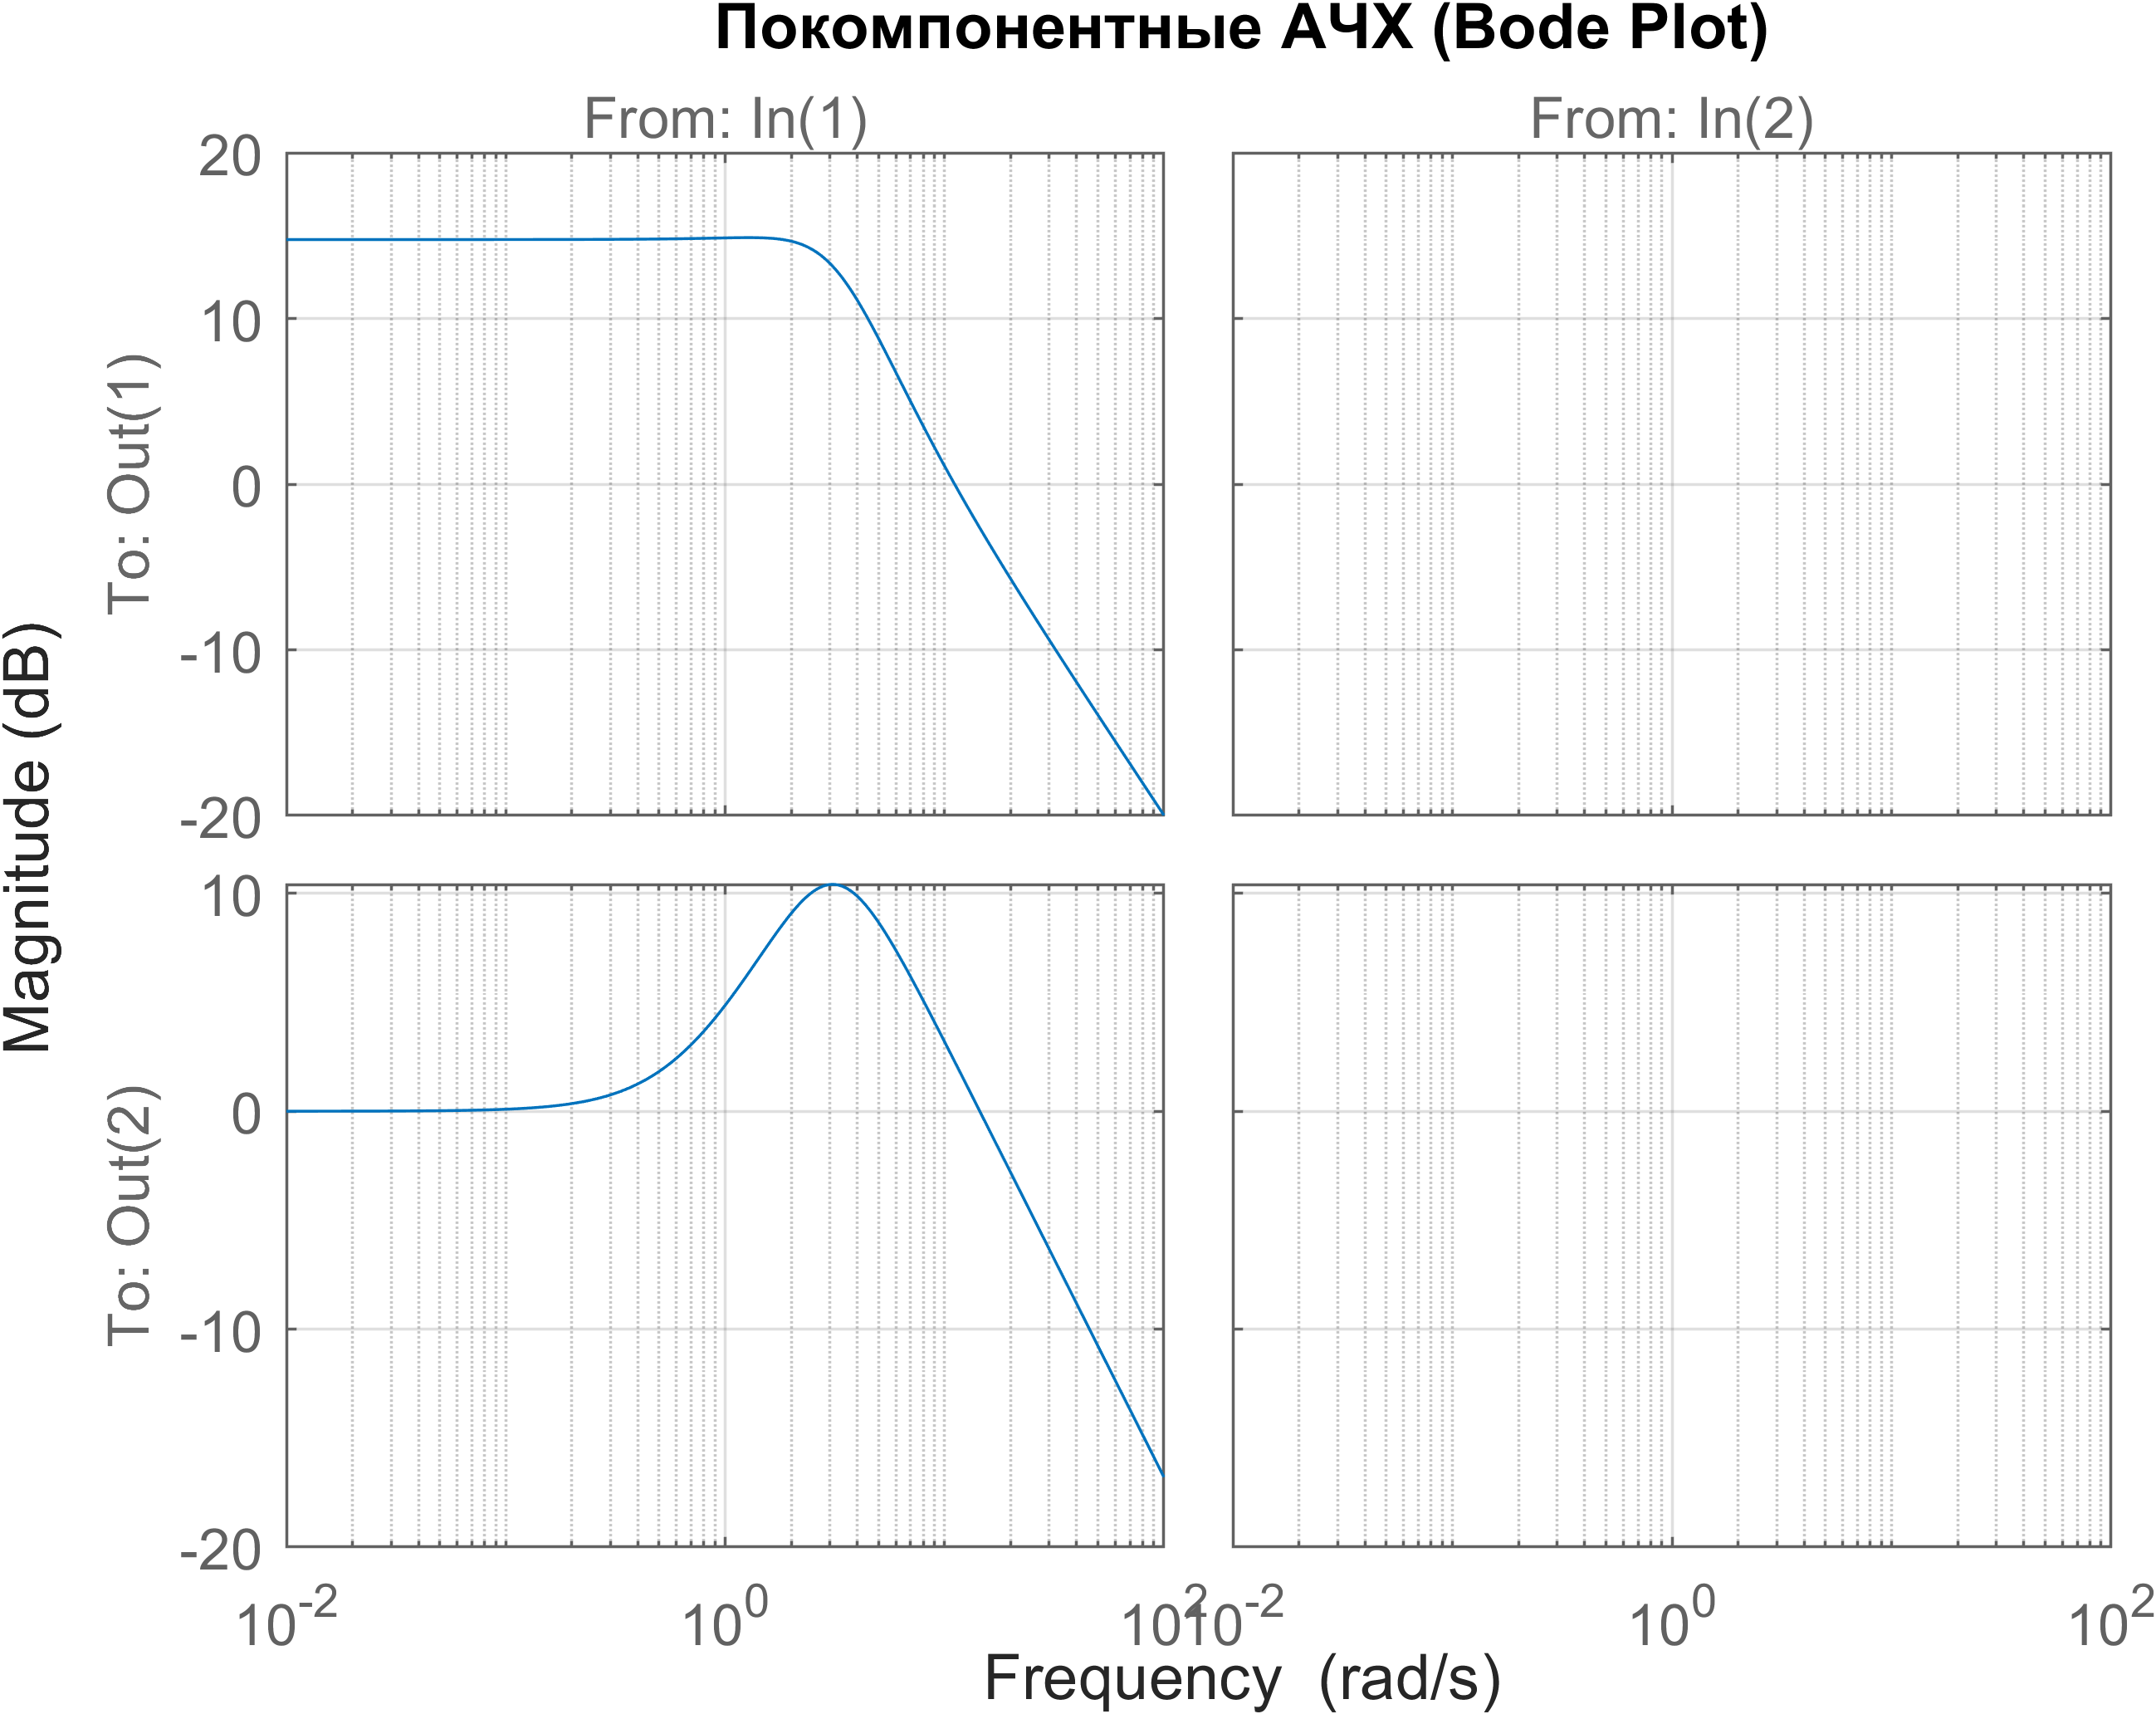
\includegraphics[width=0.8\linewidth]{figs/1_bodemag.png}
    \caption{Покомпонентные АЧХ $\underset{w\rightarrow z}{W}(s)$}
    \label{fig:1bodemag}
\end{figure}
График сингулярных чисел $\underset{w\rightarrow z}{W}(s)$ представлен на \autoref{fig:1sigma}.
\begin{figure}[H]
    \centering
    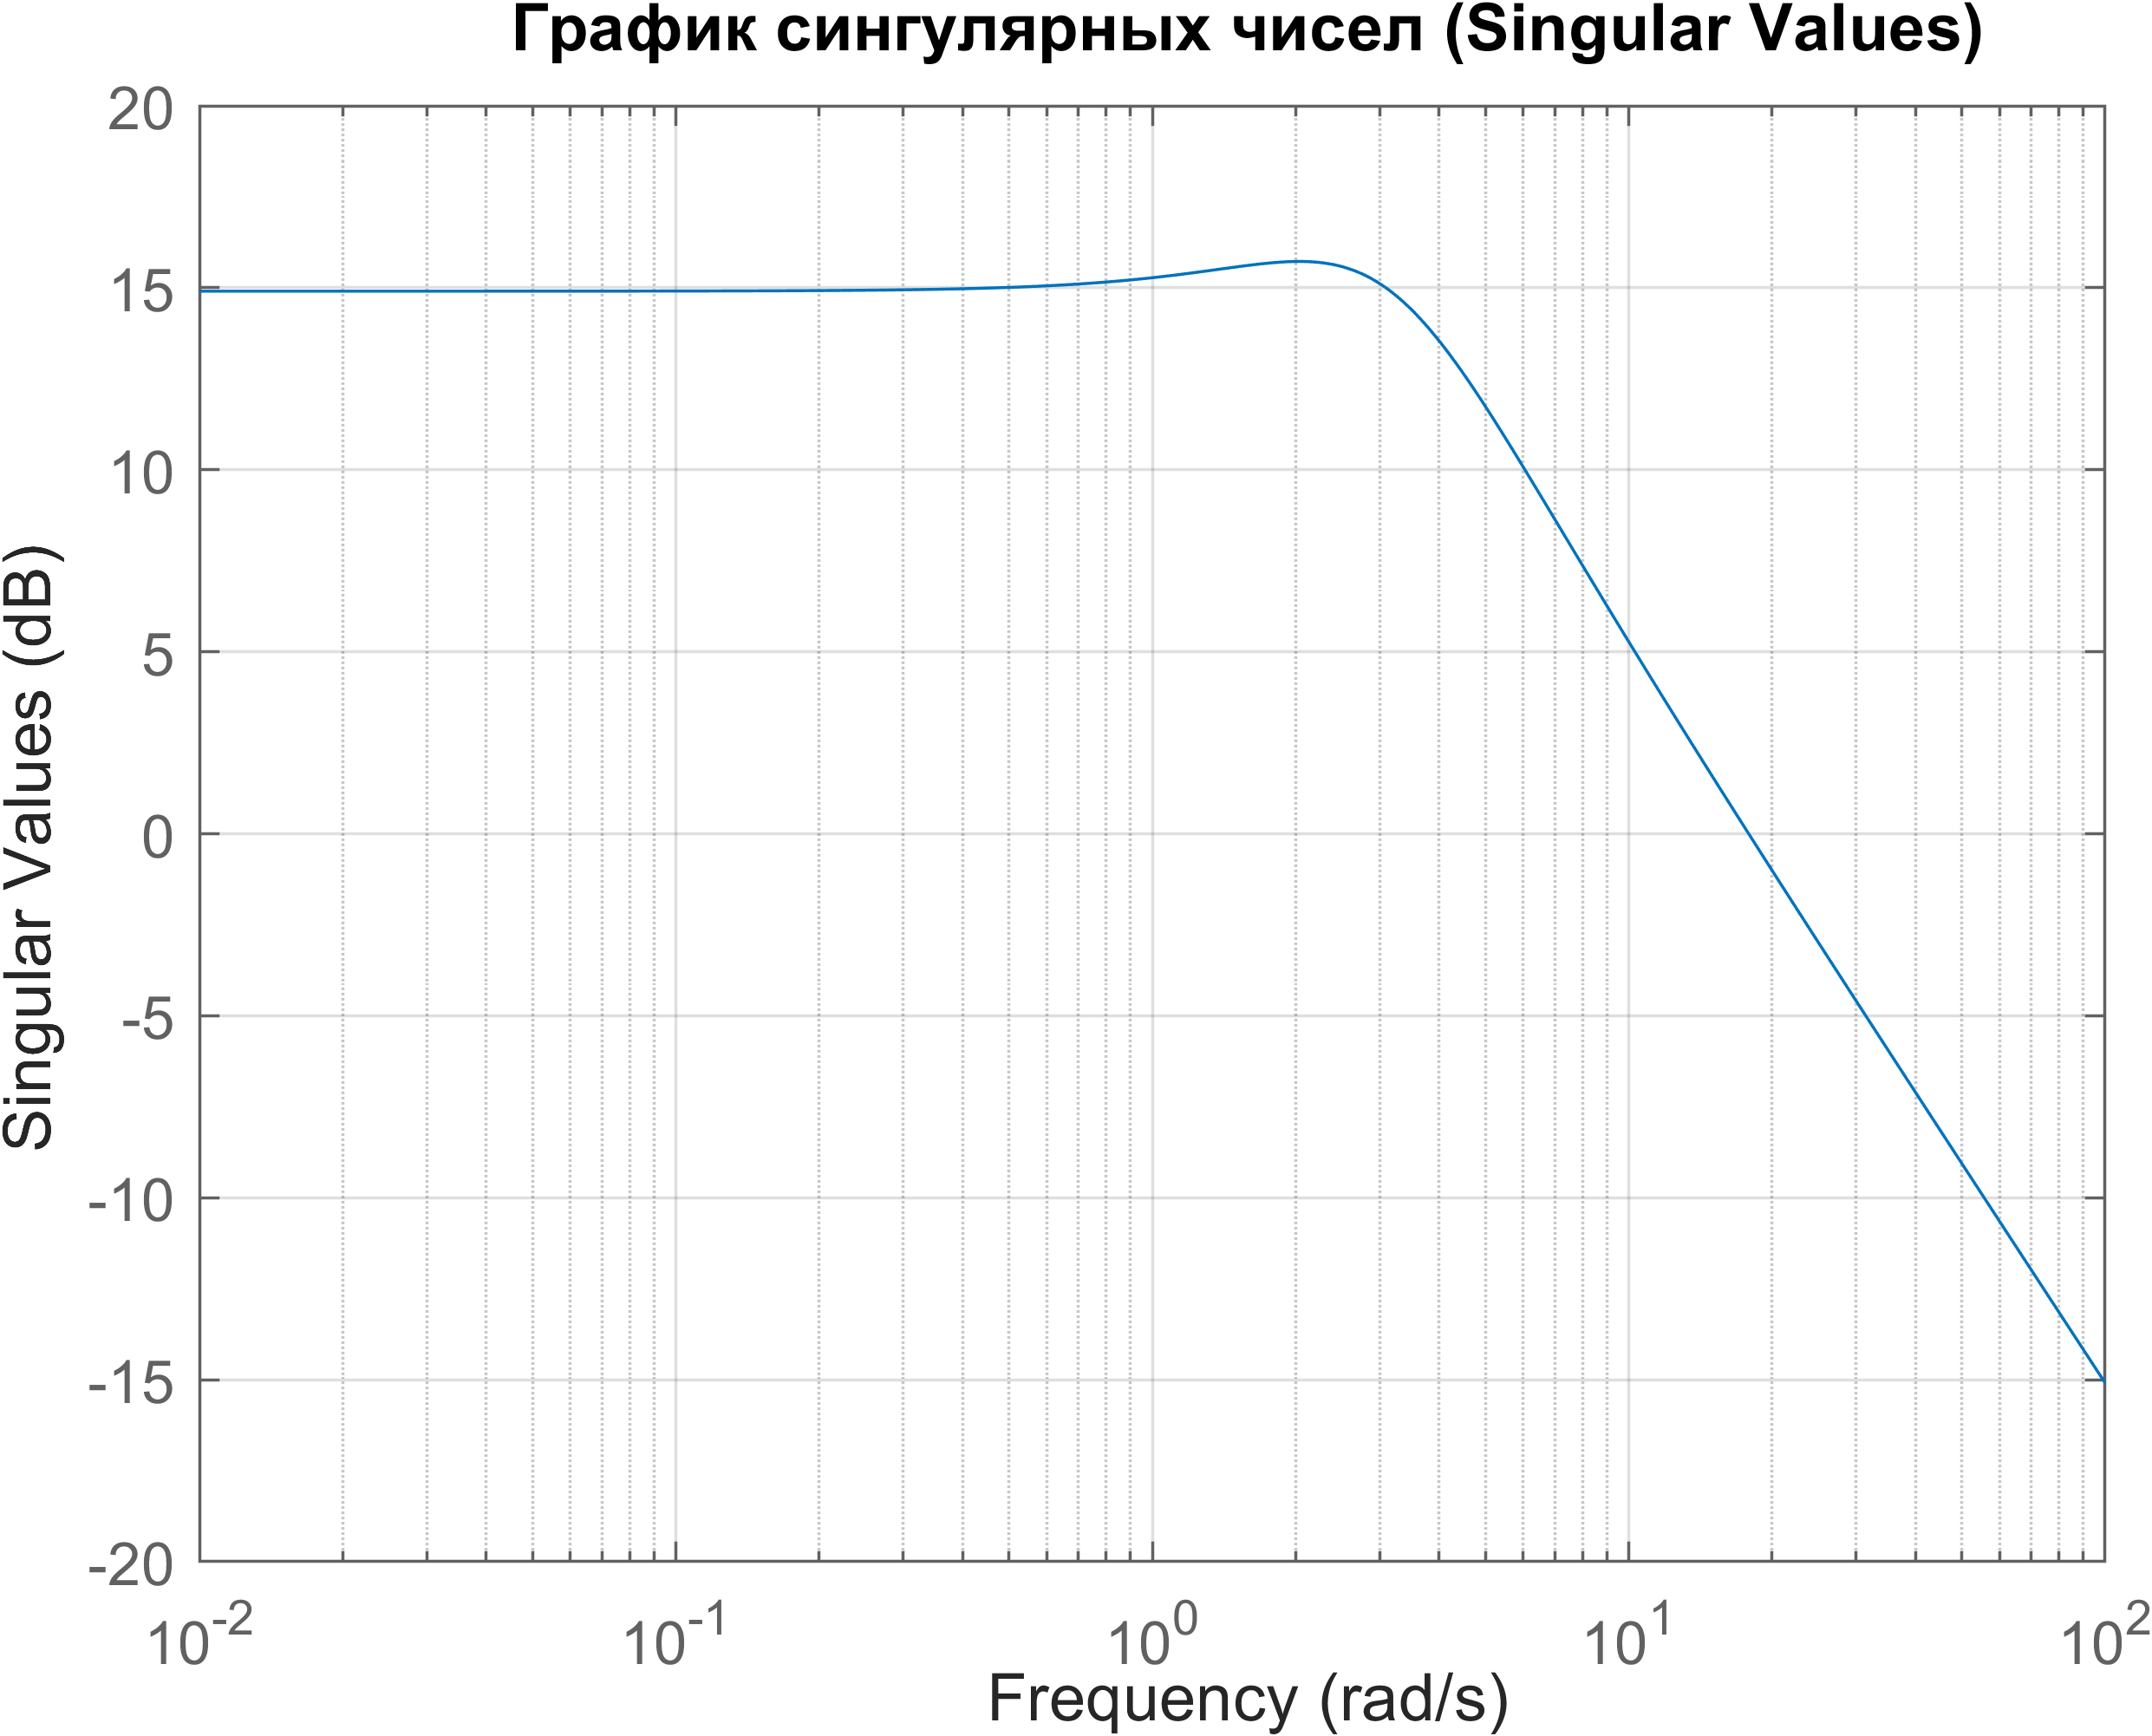
\includegraphics[width=0.8\linewidth]{figs/1_sigma.png}
    \caption{Сингулярные числа $\underset{w\rightarrow z}{W}(s)$}
    \label{fig:1sigma}
\end{figure}
\noindent Найдем нормы $\underset{w\rightarrow z}{W}(s)$:
\begin{equation*}
    ||\underset{w\rightarrow z}{W}(s)||_{H2}=8.3183,\quad
    ||\underset{w\rightarrow z}{W}(s)||_{H\infty}=6.1117.
\end{equation*}
Как видно из графика сингулярных числе, наихудшая частота возмущения $2$.
Таким образом, зададимся двумя возмущениями:
\begin{equation*}
    w_1(t)=\begin{bmatrix}
        sin(2t)\\
        0
    \end{bmatrix},\quad
    w_2(t)=\begin{bmatrix}
        sin(10t)\\
        0
    \end{bmatrix}.
\end{equation*}
\begin{figure}[H]
    \centering
    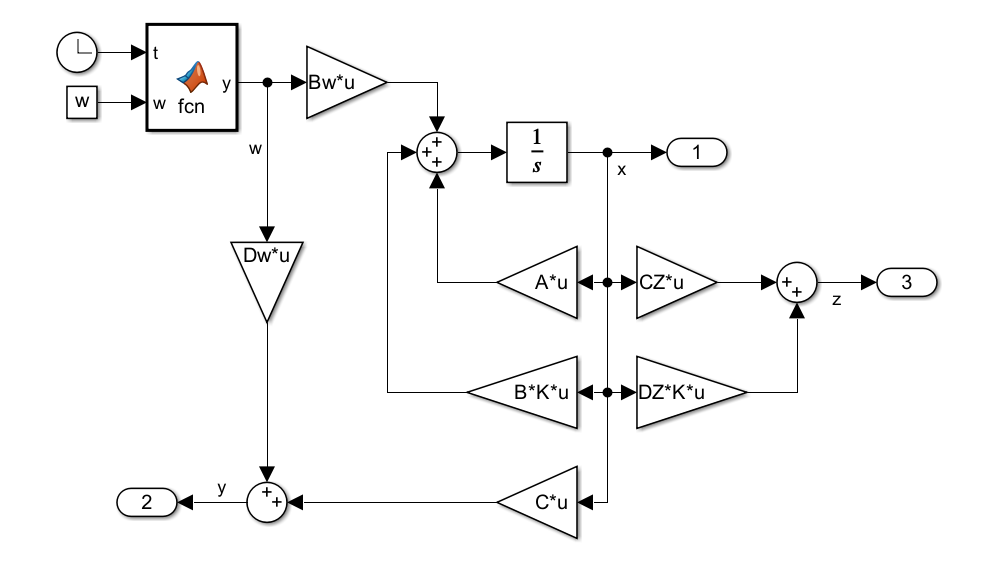
\includegraphics[width=1\linewidth]{figs/1_slx.png}
    \caption{Структурная схема системы \eqref{eq:sys} в SIMULINK}
    \label{fig:slx}
\end{figure}
С помощью SIMULINK (см. \autoref{fig:slx}) для каждого из выбранных вариантов внешнего возмущения $w$ выполним 
компьютерное моделирование замкнутой системы при нулевых начальных условиях
на объекте управления и построим графики компонент регулируемого выхода
$z(t)$, которые можно увидеть на \autoref{fig:1sim}.
\begin{figure}[H]
    \centering
    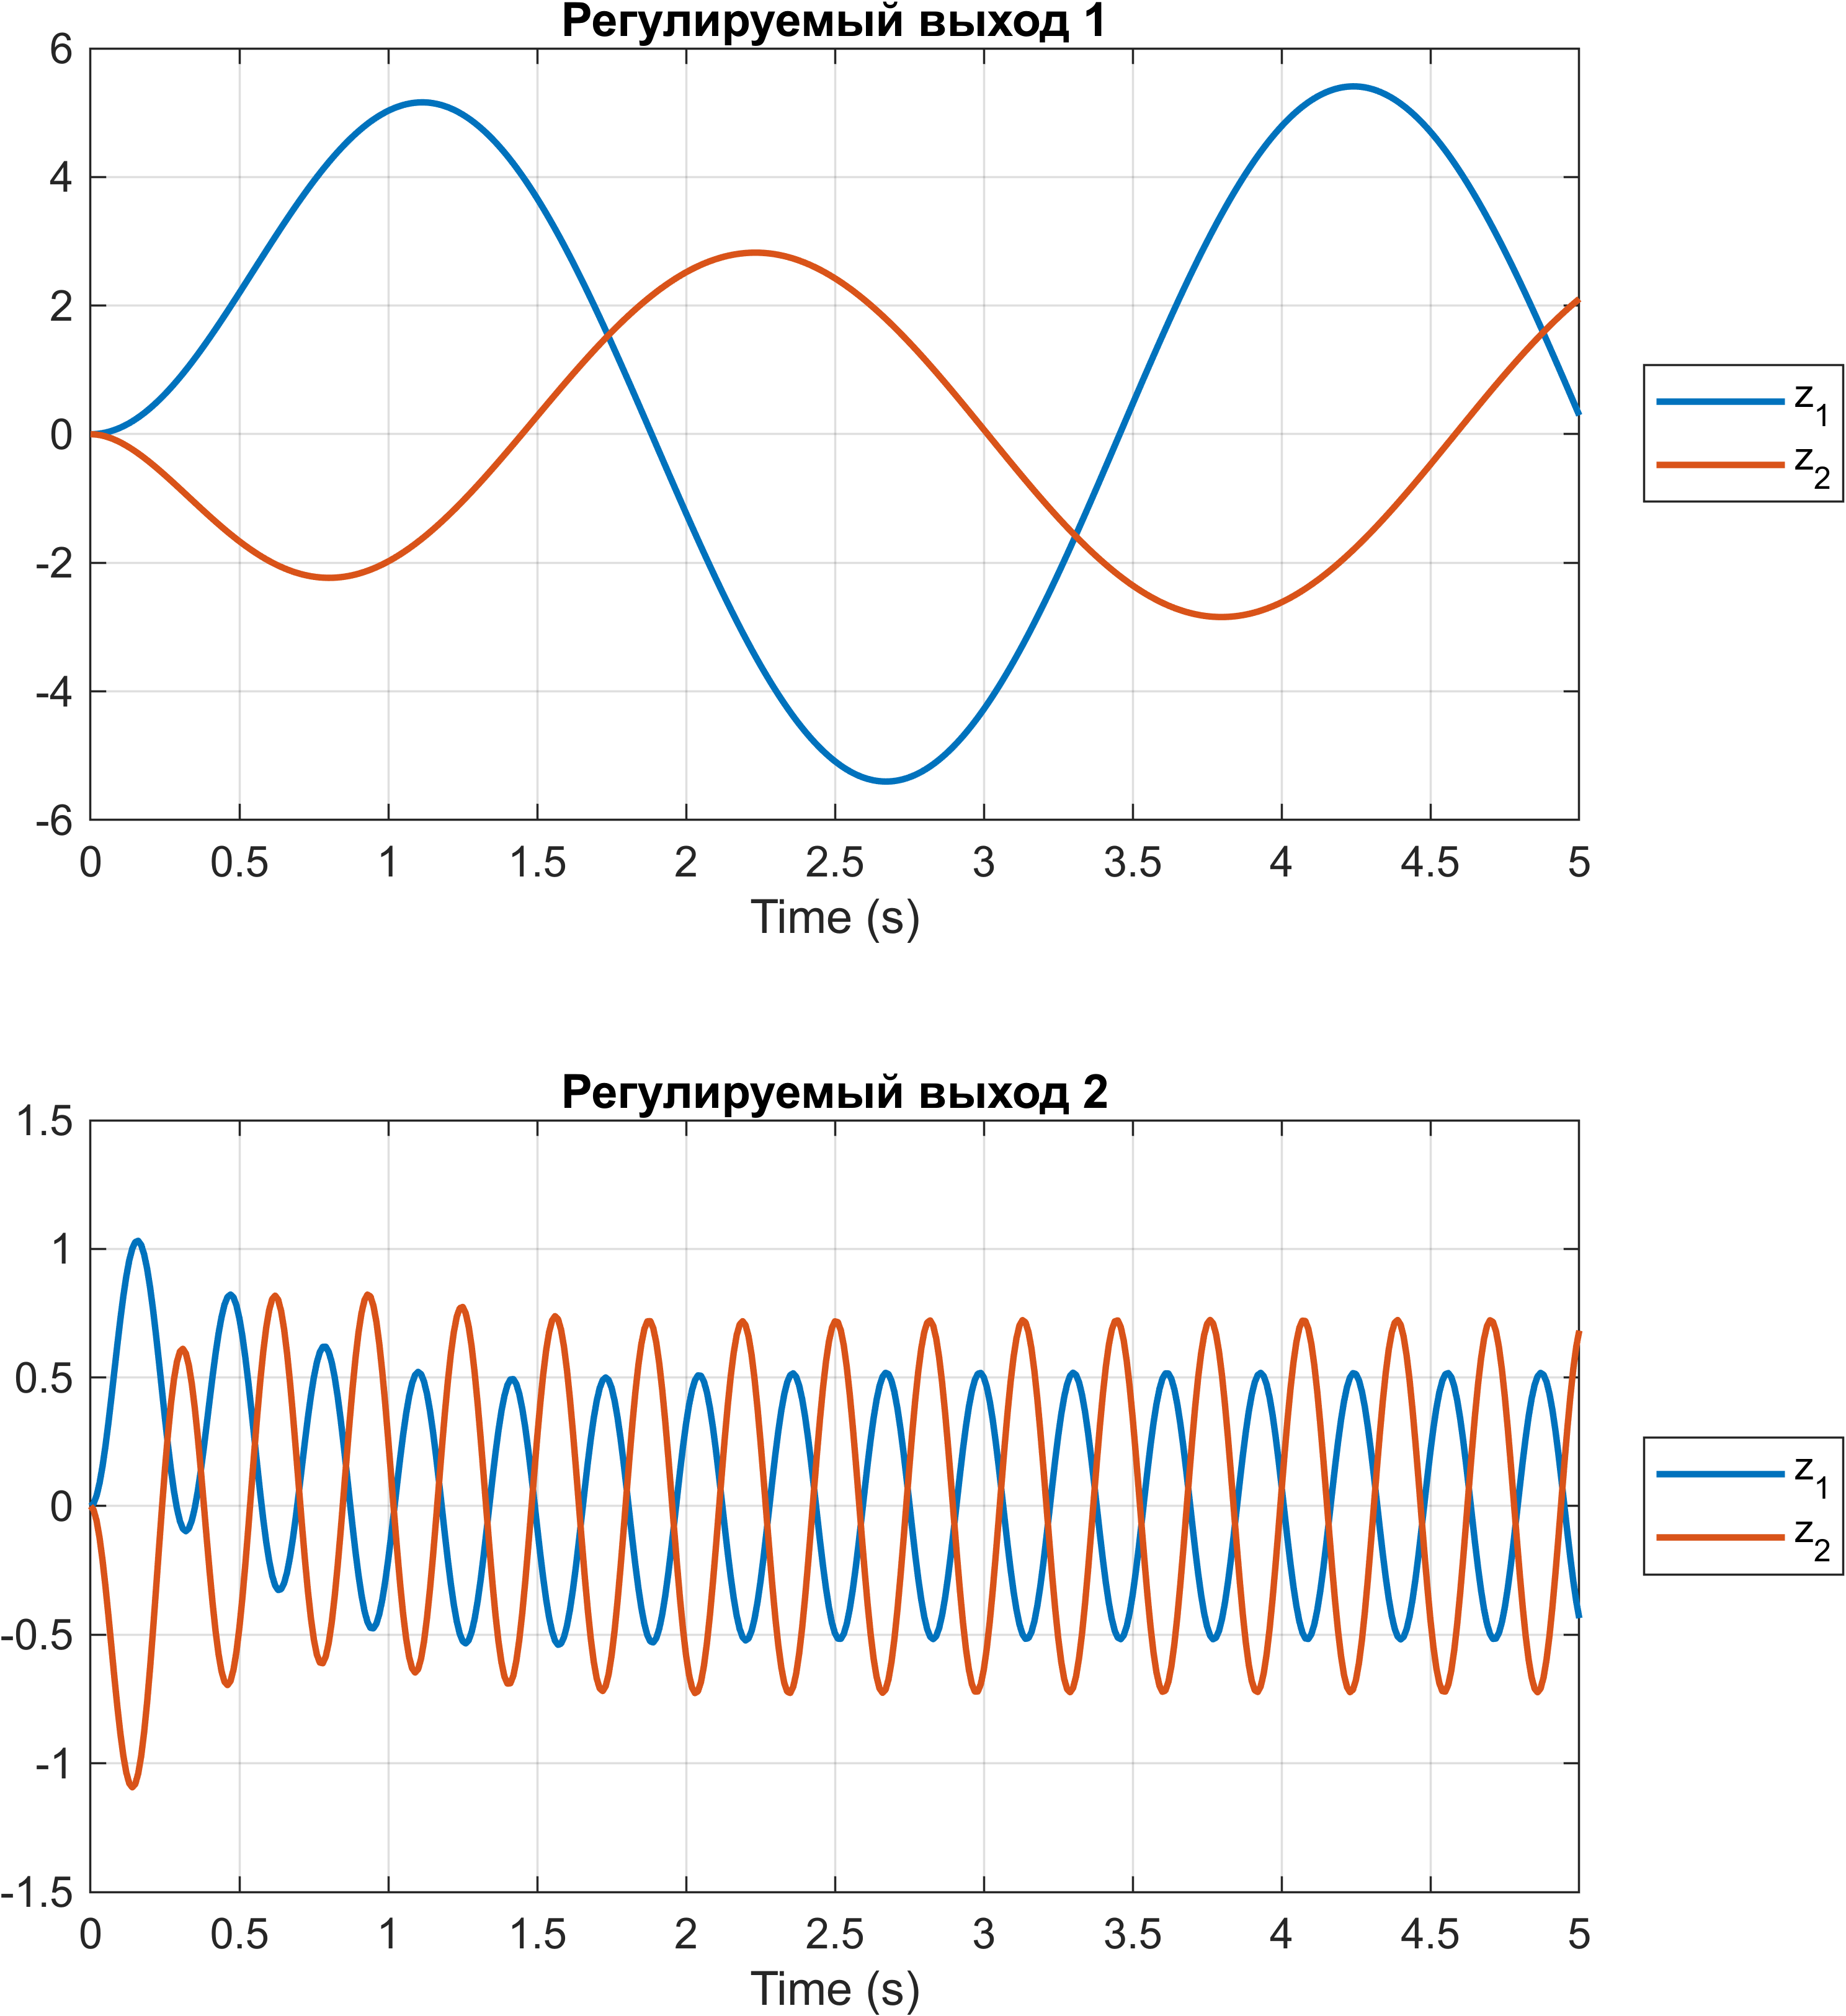
\includegraphics[width=1\linewidth]{figs/1_sim.png}
    \caption{График $z(t)$ при $w_1(t)$ и $w_2(t)$}
    \label{fig:1sim}
\end{figure}

\subsubsection{Выводы}

Из графиков видно, что полностью побороть помеху не удалось, и регулируемый выход 
колеблется около нуля, что естественно, так как нашей задачей было минимизировать норму H2. Также видно, что на 
частоте 2 амплитуда колебаний  в несколько больше чем для 10.



\subsection{Второй вариант регулируемого выхода}
\label{sec:regout2}
Аналогично синтезируем H2-регулятор вида $u=Kx$ по состоянию для $C_{Z2}$ и $D_{Z2}$.
Используя \texttt{icare} получим
\begin{equation*}
    K=\begin{bmatrix}
        -10.0000&-50.1996
    \end{bmatrix}.
\end{equation*}
Передаточная матрица замкнутой системы от внешнего возмущения $w$ к выходу $z$:
\begin{equation*}
    \underset{w\rightarrow z}{W}(s)=\begin{bmatrix}
        \dfrac{ 60 s + 12}{s^2 + 50.2 s + 10} & 0 \\[2ex]
        \dfrac{-60.2 s - 10}{s^2+50.2s+10} & 0
    \end{bmatrix}
\end{equation*}
График покомпонентных АЧХ $\underset{w\rightarrow z}{W}(s)$ представлен на \autoref{fig:2bodemag}.
\begin{figure}[H]
    \centering
    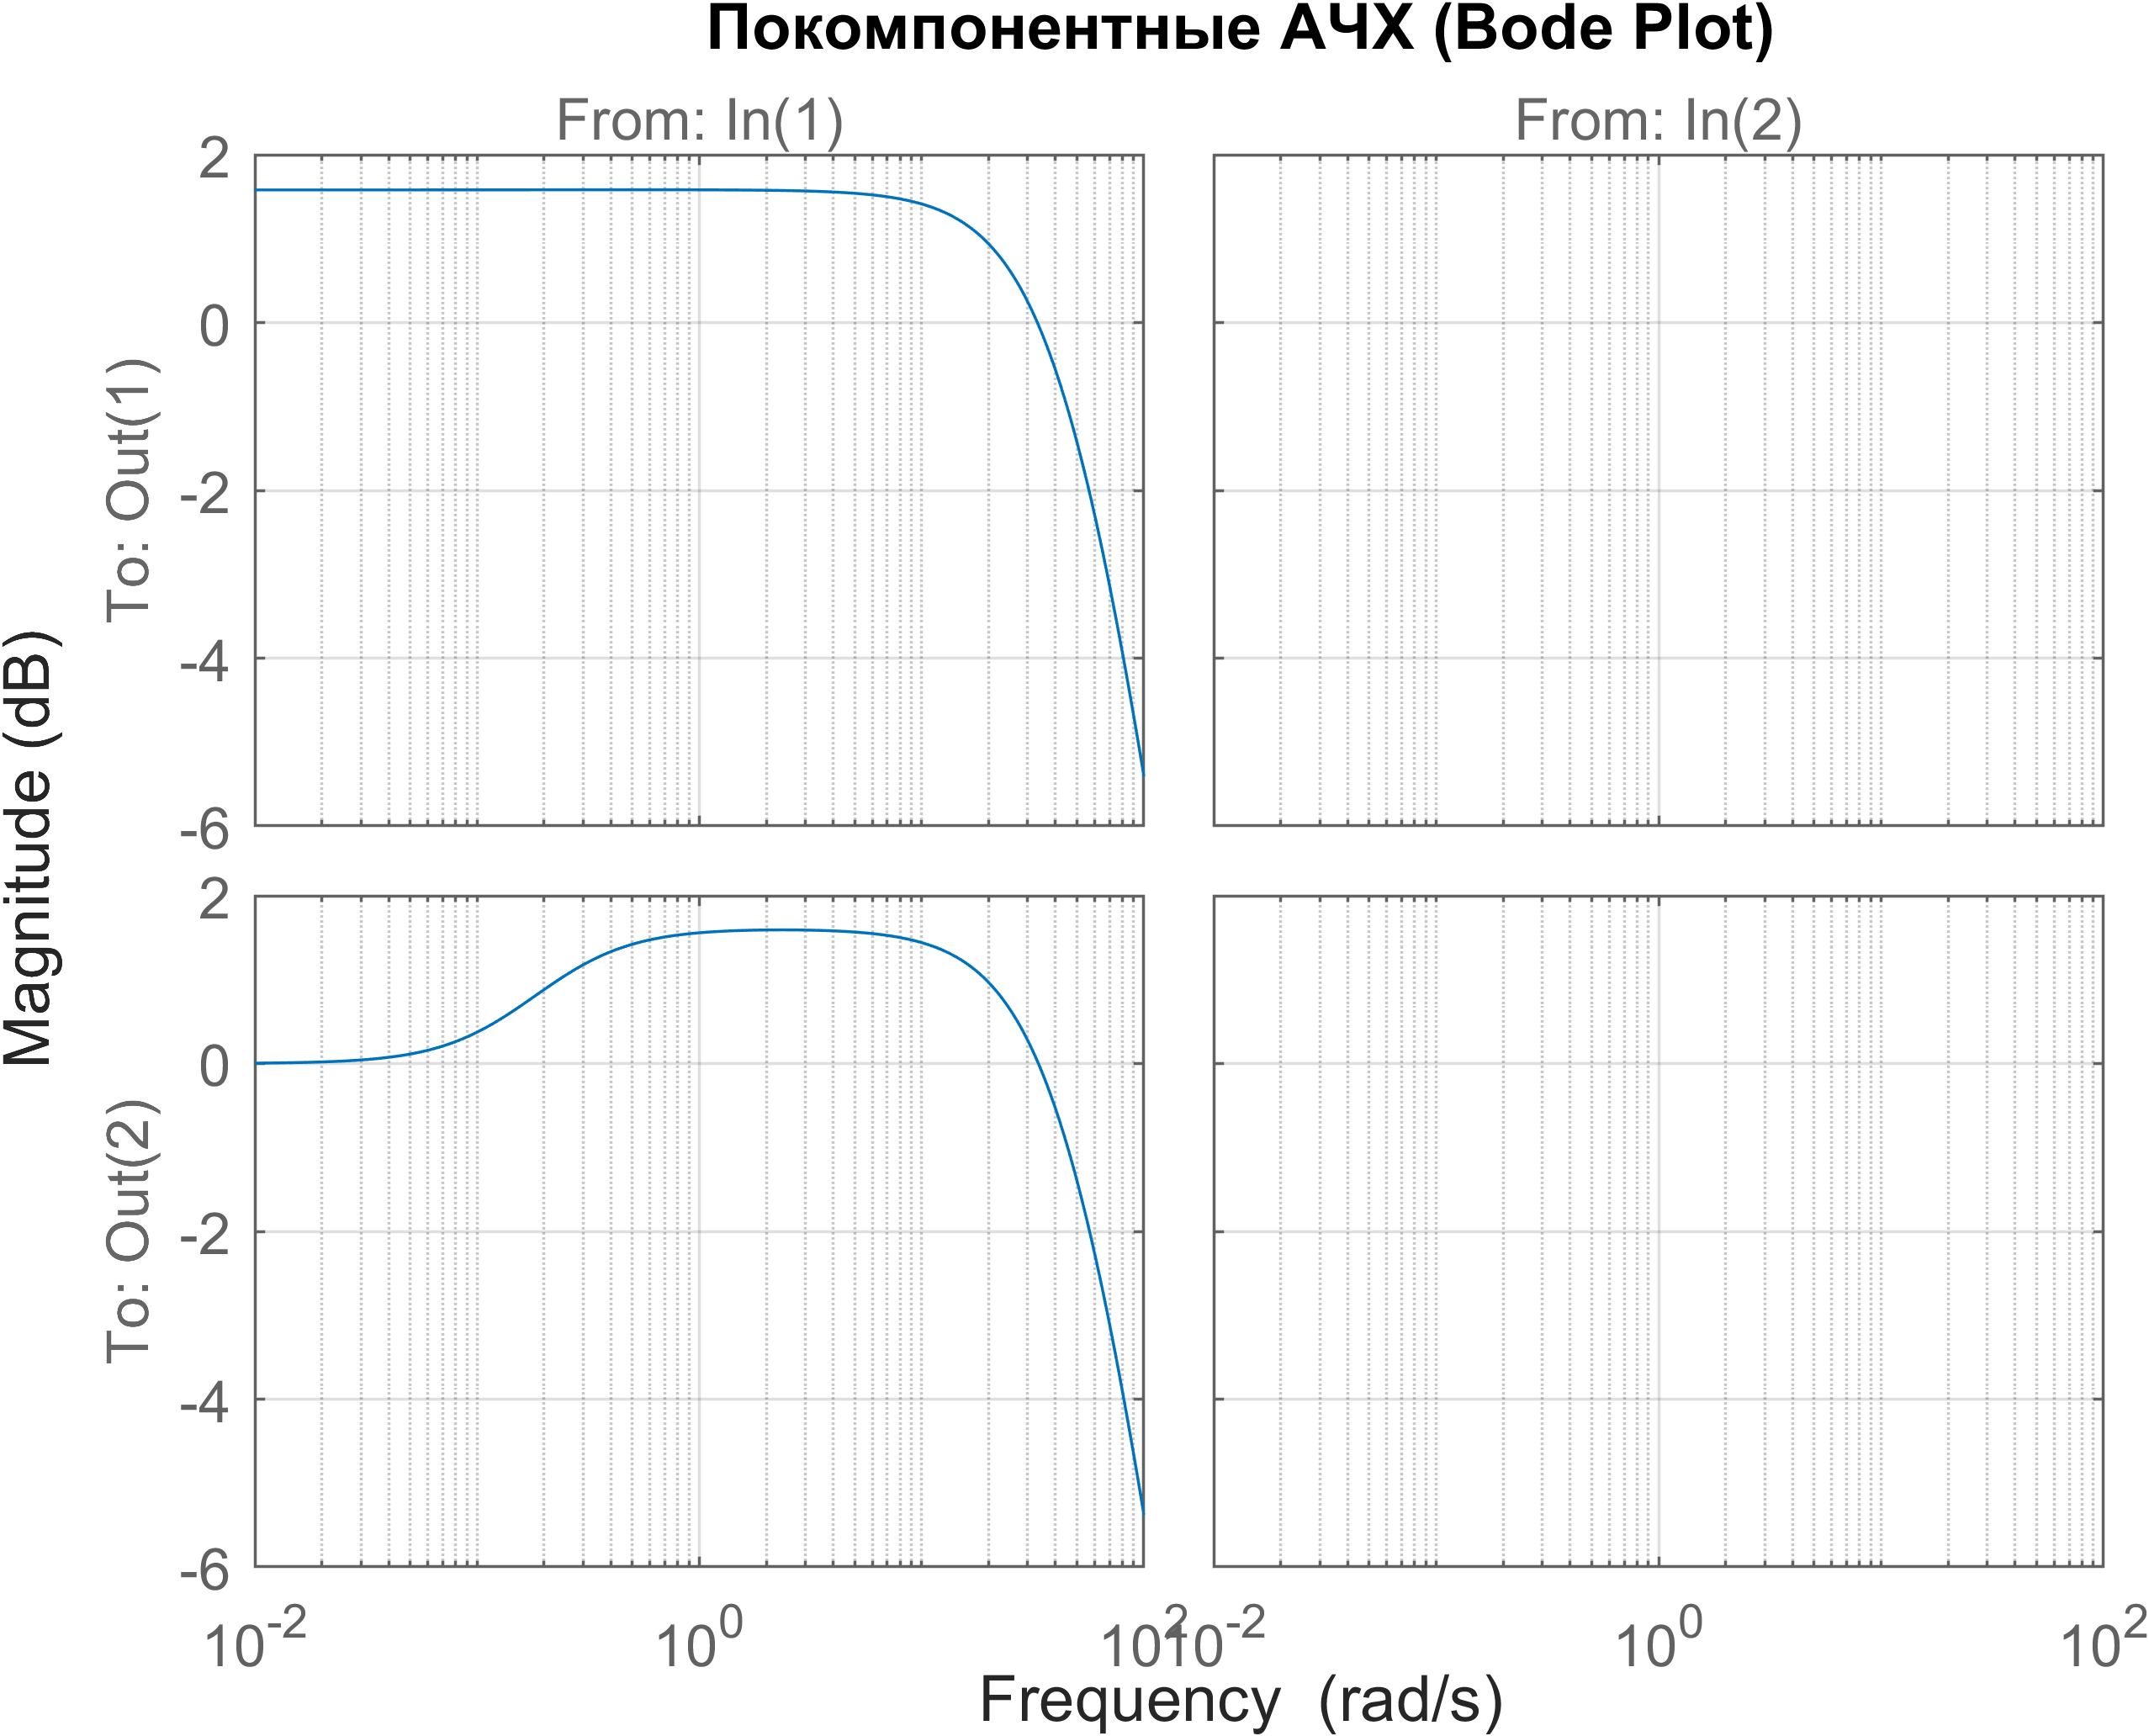
\includegraphics[width=0.8\linewidth]{figs/2_bodemag.png}
    \caption{Покомпонентные АЧХ $\underset{w\rightarrow z}{W}(s)$}
    \label{fig:2bodemag}
\end{figure}
График сингулярных чисел $\underset{w\rightarrow z}{W}(s)$ представлен на \autoref{fig:2sigma}.
\begin{figure}[H]
    \centering
    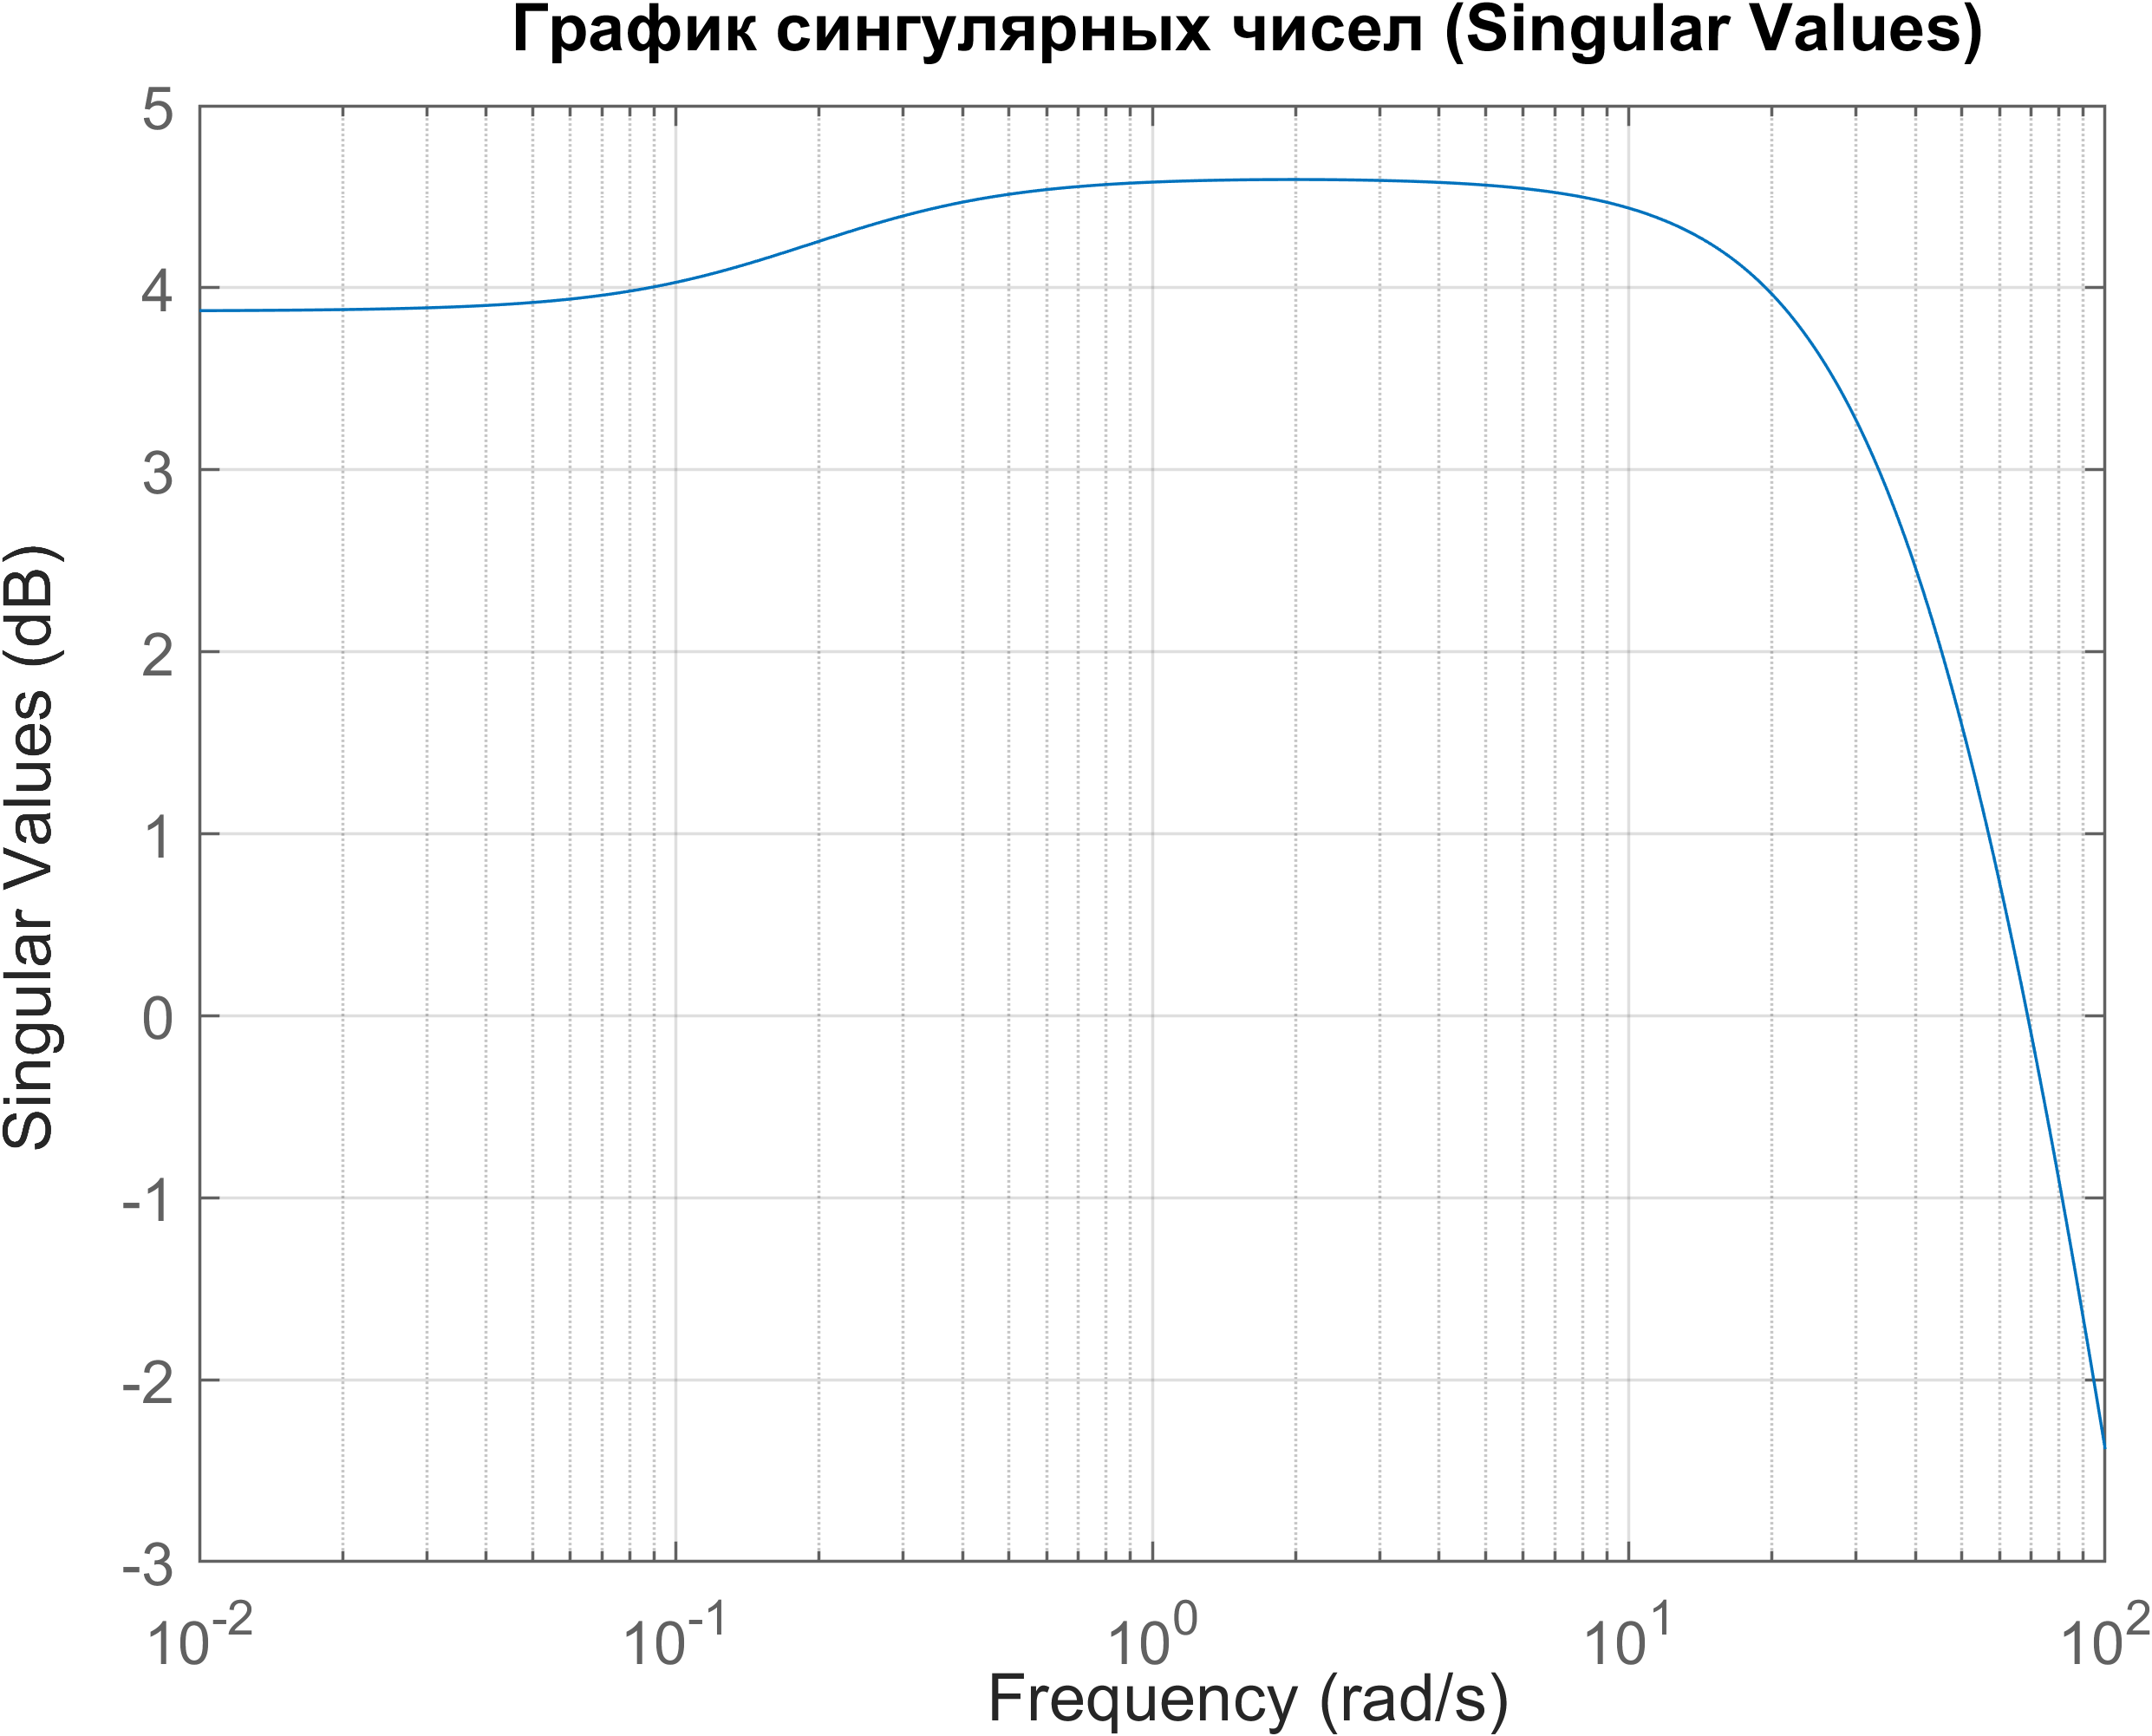
\includegraphics[width=0.8\linewidth]{figs/2_sigma.png}
    \caption{Сингулярные числа $\underset{w\rightarrow z}{W}(s)$}
    \label{fig:2sigma}
\end{figure}
Найдем нормы $\underset{w\rightarrow z}{W}(s)$:
\begin{equation*}
    ||\underset{w\rightarrow z}{W}(s)||_{H2}=8.4968,\quad
    ||\underset{w\rightarrow z}{W}(s)||_{H\infty}=1.6972.
\end{equation*}
Как видно из графика сингулярных числе, наихудшая частота возмущения около $1$. 
Таким образом, зададимся двумя возмущениями:
\begin{equation*}
    w_1(t)=\begin{bmatrix}
        sin(t)\\
        0
    \end{bmatrix},\quad
    w_2(t)=\begin{bmatrix}
        sin(15t)\\
        0
    \end{bmatrix}.
\end{equation*}
С помощью SIMULINK (см. \autoref{fig:slx}) для каждого из выбранных вариантов внешнего возмущения $w$ выполним 
компьютерное моделирование замкнутой системы при нулевых начальных условиях
на объекте управления и построим графики компонент регулируемого выхода
$z(t)$, которые можно увидеть на \autoref{fig:2sim}.
\begin{figure}[H]
    \centering
    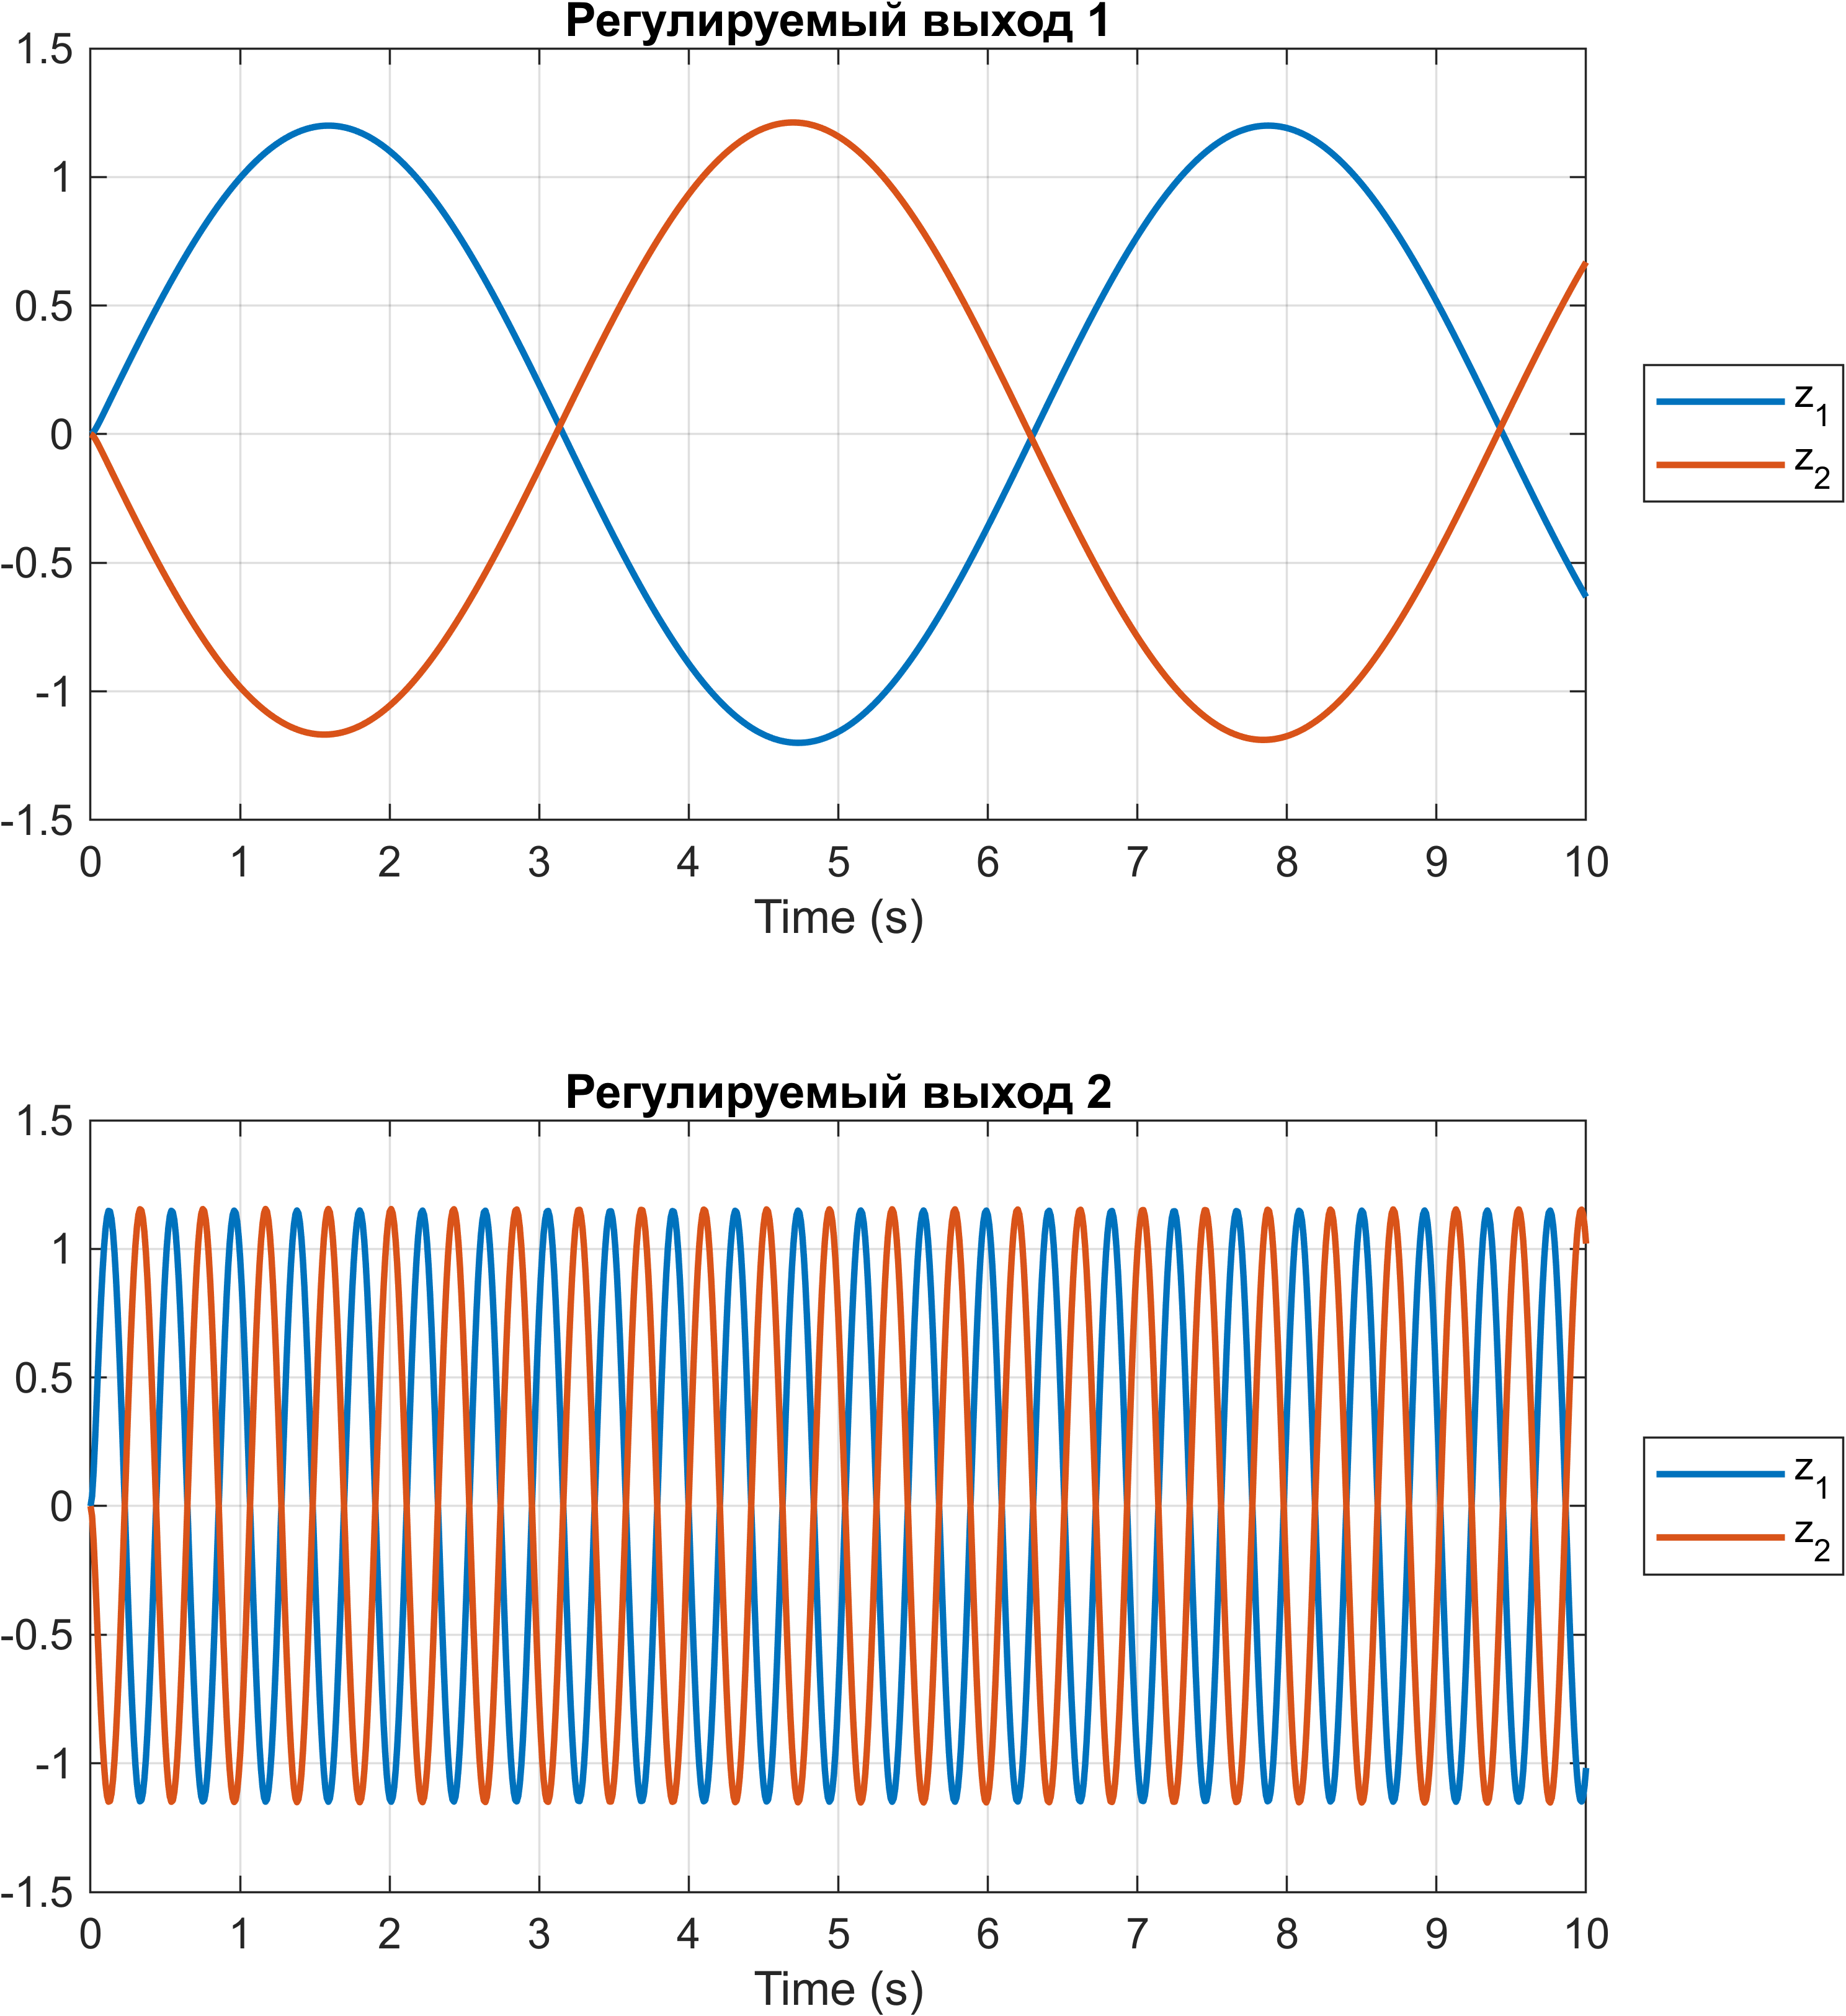
\includegraphics[width=1\linewidth]{figs/2_sim.png}
    \caption{График $z(t)$ при $w_1(t)$ и $w_2(t)$}
    \label{fig:2sim}
\end{figure}

\subsubsection{Выводы}

Из графиков видно, что полностью побороть помеху не удалось, и регулируемый выход 
колеблется около нуля, аналогично первому варианту. Также видно, что на 
частоте 1 амплитуда колебаний в несколько больше чем для 15.





\section{Синтез H2-регулятора по выходу}

\subsection{Первый вариант регулируемого выхода}

Так как при построении H2-регулятора по выходу действует separation principle,
в качестве $K$ возьмем матрицу из \autoref{sec:regout1}:
\begin{equation*}
    K=\begin{bmatrix}
        -10.0000&-4.4721
    \end{bmatrix}.
\end{equation*}
Синтезируем H2-наблюдатель путем решения матричного уравнения Риккати:
\begin{equation}
    \label{eq:ric2}
    AP+PA^T+B_wB_w^T-PC^T(D_wD_w^T)^{-1}CP=0,\quad L=-PC^T(D_wD_w^T)^{-1}.
\end{equation}
Используя \texttt{icare} получим
\begin{equation*}
    L=\begin{bmatrix}
        -1.7321 &
        -1.0000
    \end{bmatrix}^T.
\end{equation*}
Получим систему, где вход $w$ и выход $z$. Имеем две системы: объекта и наблюдателя:
\begin{equation*}
    \begin{cases}
        \dot x=Ax+Bu+B_ww\\
        y=Cx+D_ww\\
        z=C_Zx+D_Zu
    \end{cases},\quad
    \begin{cases}
        \dot{\hat x}=A\hat x+Bu+L(y-\hat y)\\
        \hat y=C\hat x
    \end{cases},
\end{equation*}
подставив управление $u=K\hat x$ и вход $y$ в наблюдатель, получим:
\begin{equation*}
    \dot{\hat x}=(A+BK+LC)\hat x-LCx-LD_ww,
\end{equation*}
подставив $u=K\hat x$ в систему объекта, получим:
\begin{equation*}
    \dot x=Ax+BK\hat x+B_ww,
\end{equation*}
\begin{equation*}
    z=C_Zx+D_ZK\hat x.
\end{equation*}
Из последних двух уравнений можно получить желаемую систему, взяв за состояние вектор 
$s=\begin{bmatrix}
    x & \hat x
\end{bmatrix}$:
\begin{equation*}
    \begin{cases}
        \dot s=\begin{bmatrix}
            A & BK \\ -LC & A+BK+LC
        \end{bmatrix}s+\begin{bmatrix}
            B \\ -LD_w
        \end{bmatrix}w,\\[3ex]
        z=\begin{bmatrix}
            C_Z & D_ZK
        \end{bmatrix}s.
    \end{cases}
\end{equation*}
Тогда передаточная матрица, полученная через tf в MATLAB, замкнутой системы от внешнего возмущения $w$ к выходу $z$:
\begin{equation*}
    \underset{w\rightarrow z}{W}(s)=\begin{bmatrix}
        \underset{w\rightarrow z}{W_1}(s) & \underset{w\rightarrow z}{W_2}(s)\\
        \underset{w\rightarrow z}{W_3}(s) & \underset{w\rightarrow z}{W_4}(s)
    \end{bmatrix},
\end{equation*}
где
\begin{gather*}
    \underset{w\rightarrow z}{W_1}(s)=\dfrac{10 s^3 + (63.38-5i) s^2 + (200.8-22.36i) s + (147.4-17.36i)}{s^4 + (5.338-0.5i) s^3 + (14.74-1.736i) s^2 + (12.53-2.764i) s + (8.66+5i)}\\
    \underset{w\rightarrow z}{W_2}(s)=\dfrac{-(125.3-27.64i) s - (86.6+50i)}{s^4 + (5.338-0.5i) s^3 + (14.74-1.736i) s^2 + (12.53-2.764i) s + (8.66+5i)}\\
    \underset{w\rightarrow z}{W_3}(s)=\dfrac{-(12.53-2.764i) s^2 - (21.19+2.236i) s - (8.66+5i)}{s^4 + (5.338-0.5i) s^3 + (14.74-1.736i) s^2 + (12.53-2.764i) s + (8.66+5i)} \\
    \hspace*{-1.5cm} \underset{w\rightarrow z}{W_4}(s)=\dfrac{-(12.53-2.764i) s^3 - (8.66+5i) s^2 + (2.714\cdot 10^{-16}+i4.647\cdot 10^{-16}) s - (8.823\cdot 10^{-17}-4.099\cdot 10^{-16}i)}{s^4 + (5.338-0.5i) s^3 + (14.74-1.736i) s^2 + (12.53-2.764i) s + (8.66+5i)}
\end{gather*}
График покомпонентных АЧХ $\underset{w\rightarrow z}{W}(s)$ представлен на \autoref{fig:3bodemag}.
\begin{figure}[H]
    \centering
    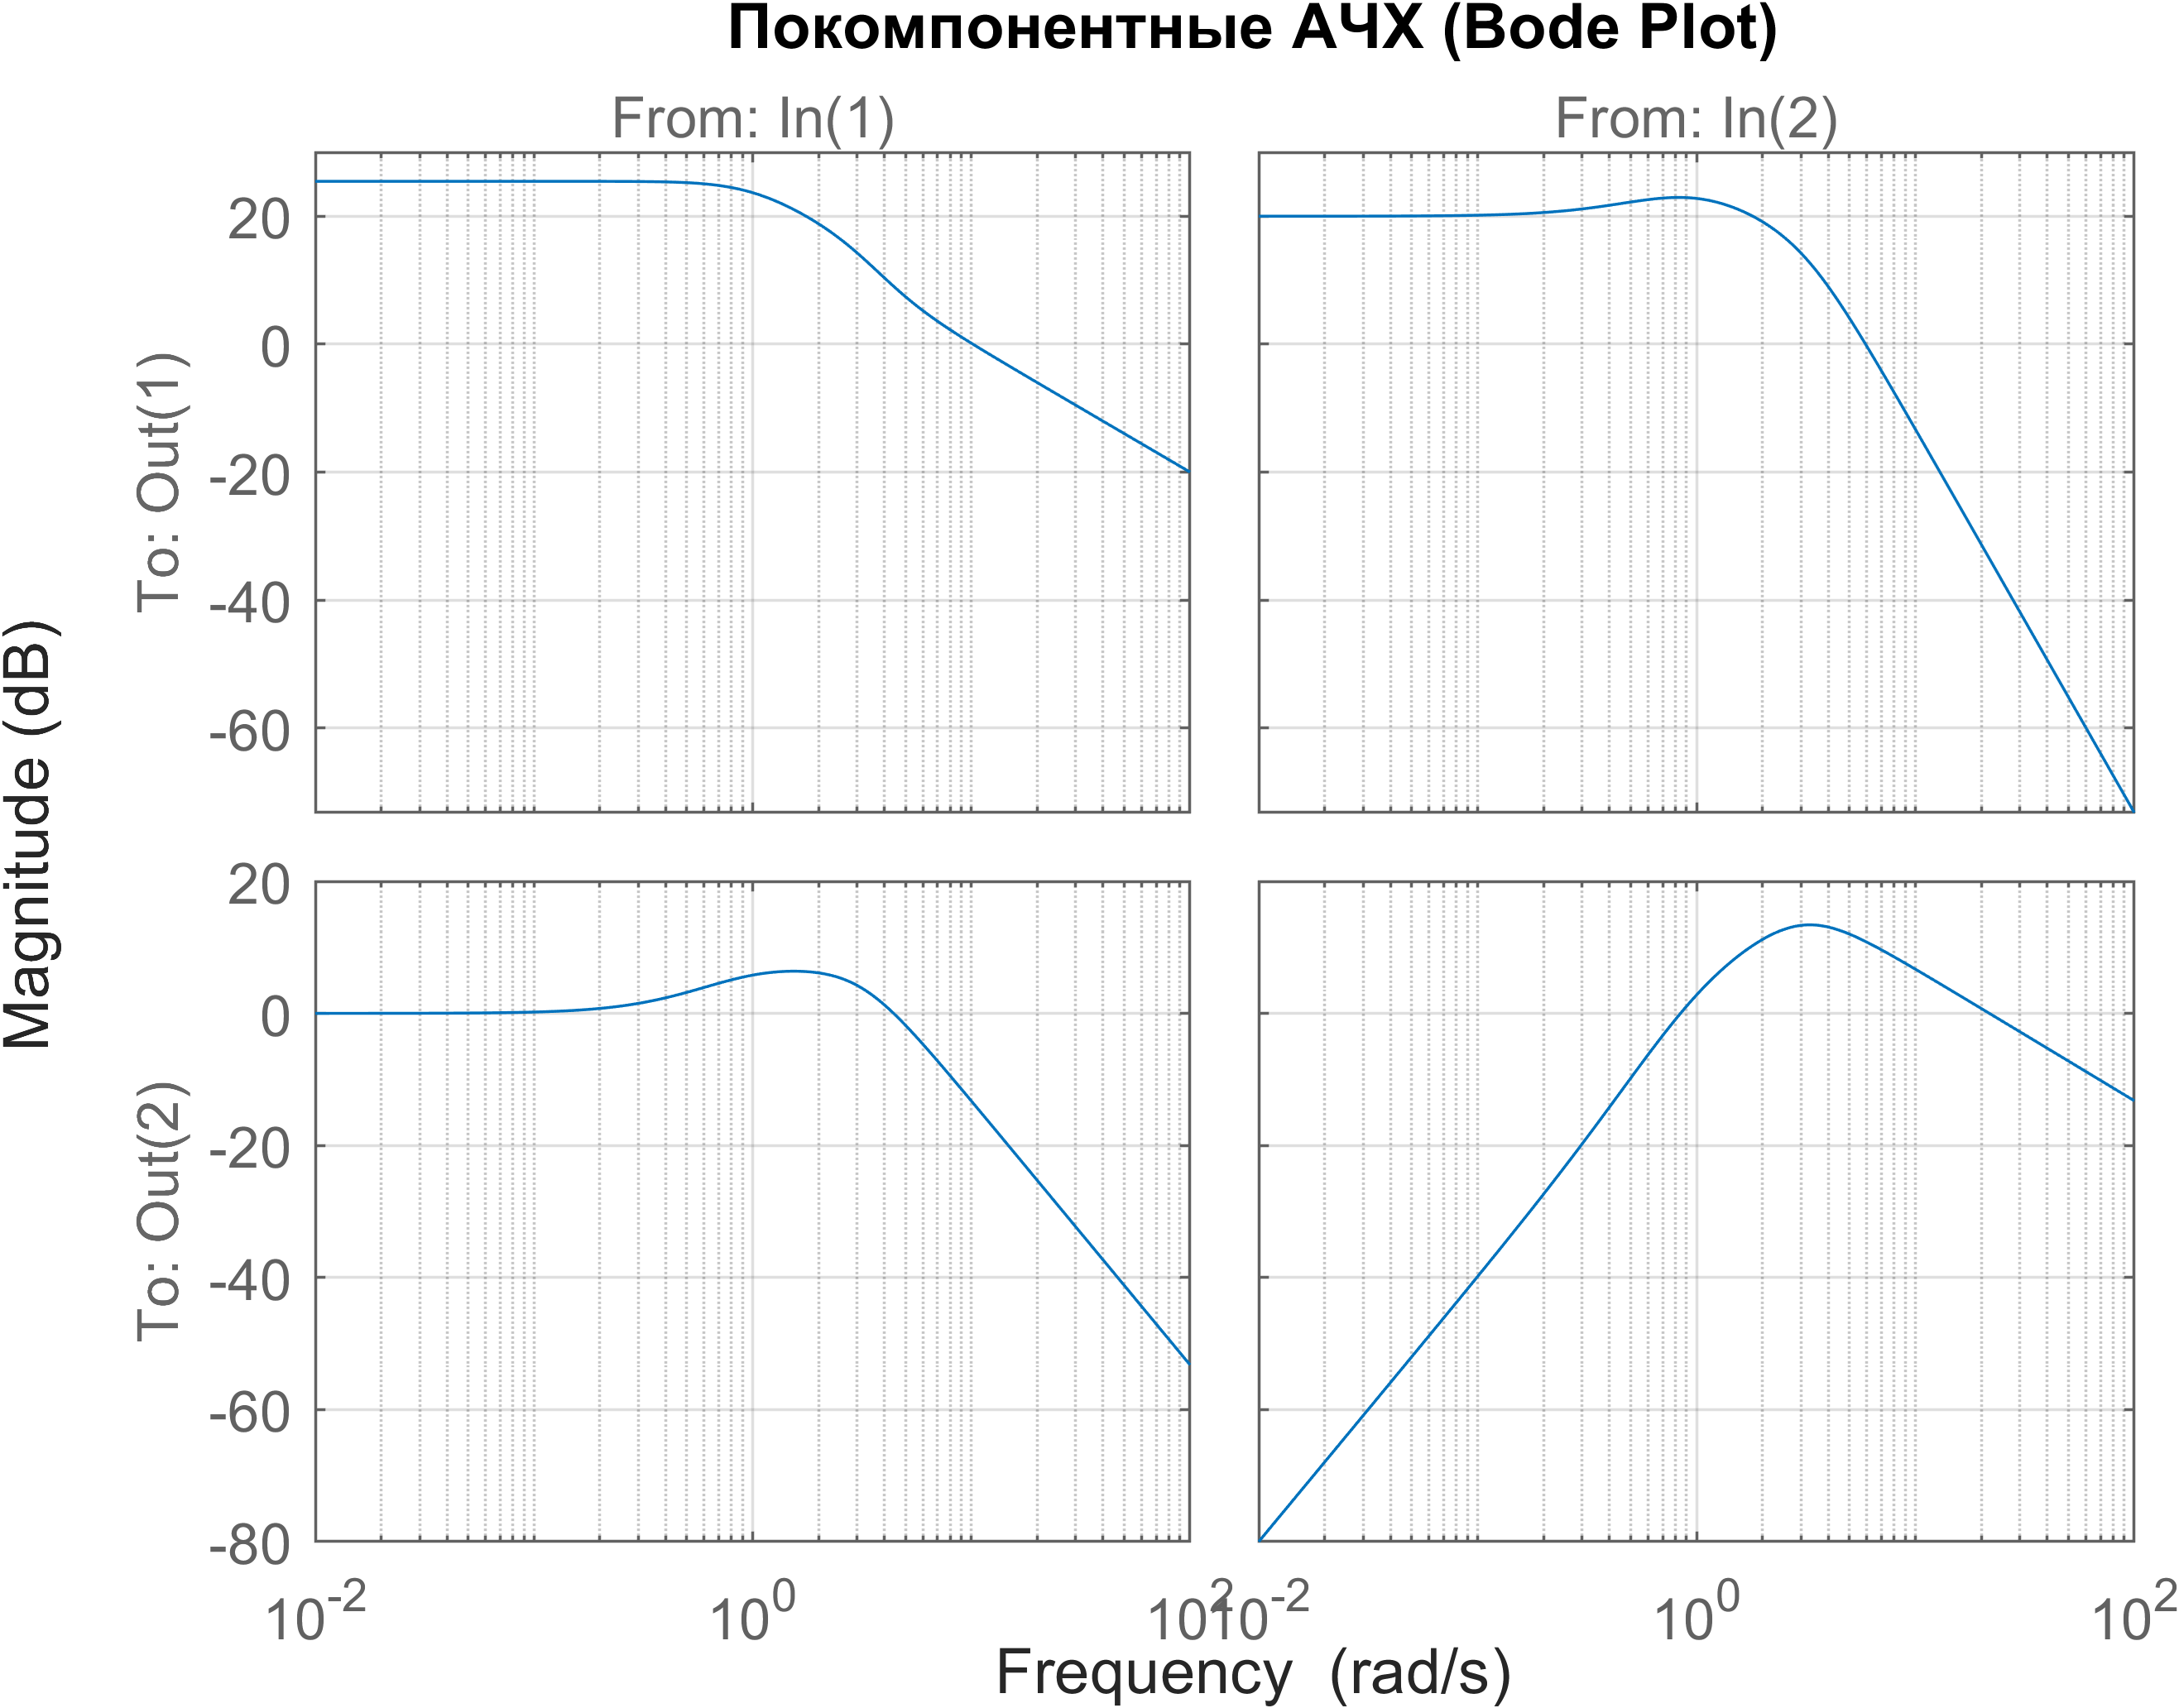
\includegraphics[width=0.7\linewidth]{figs/3_bodemag.png}
    \caption{Покомпонентные АЧХ $\underset{w\rightarrow z}{W}(s)$}
    \label{fig:3bodemag}
\end{figure}
График сингулярных чисел $\underset{w\rightarrow z}{W}(s)$ представлен на \autoref{fig:3sigma}.
\begin{figure}[H]
    \centering
    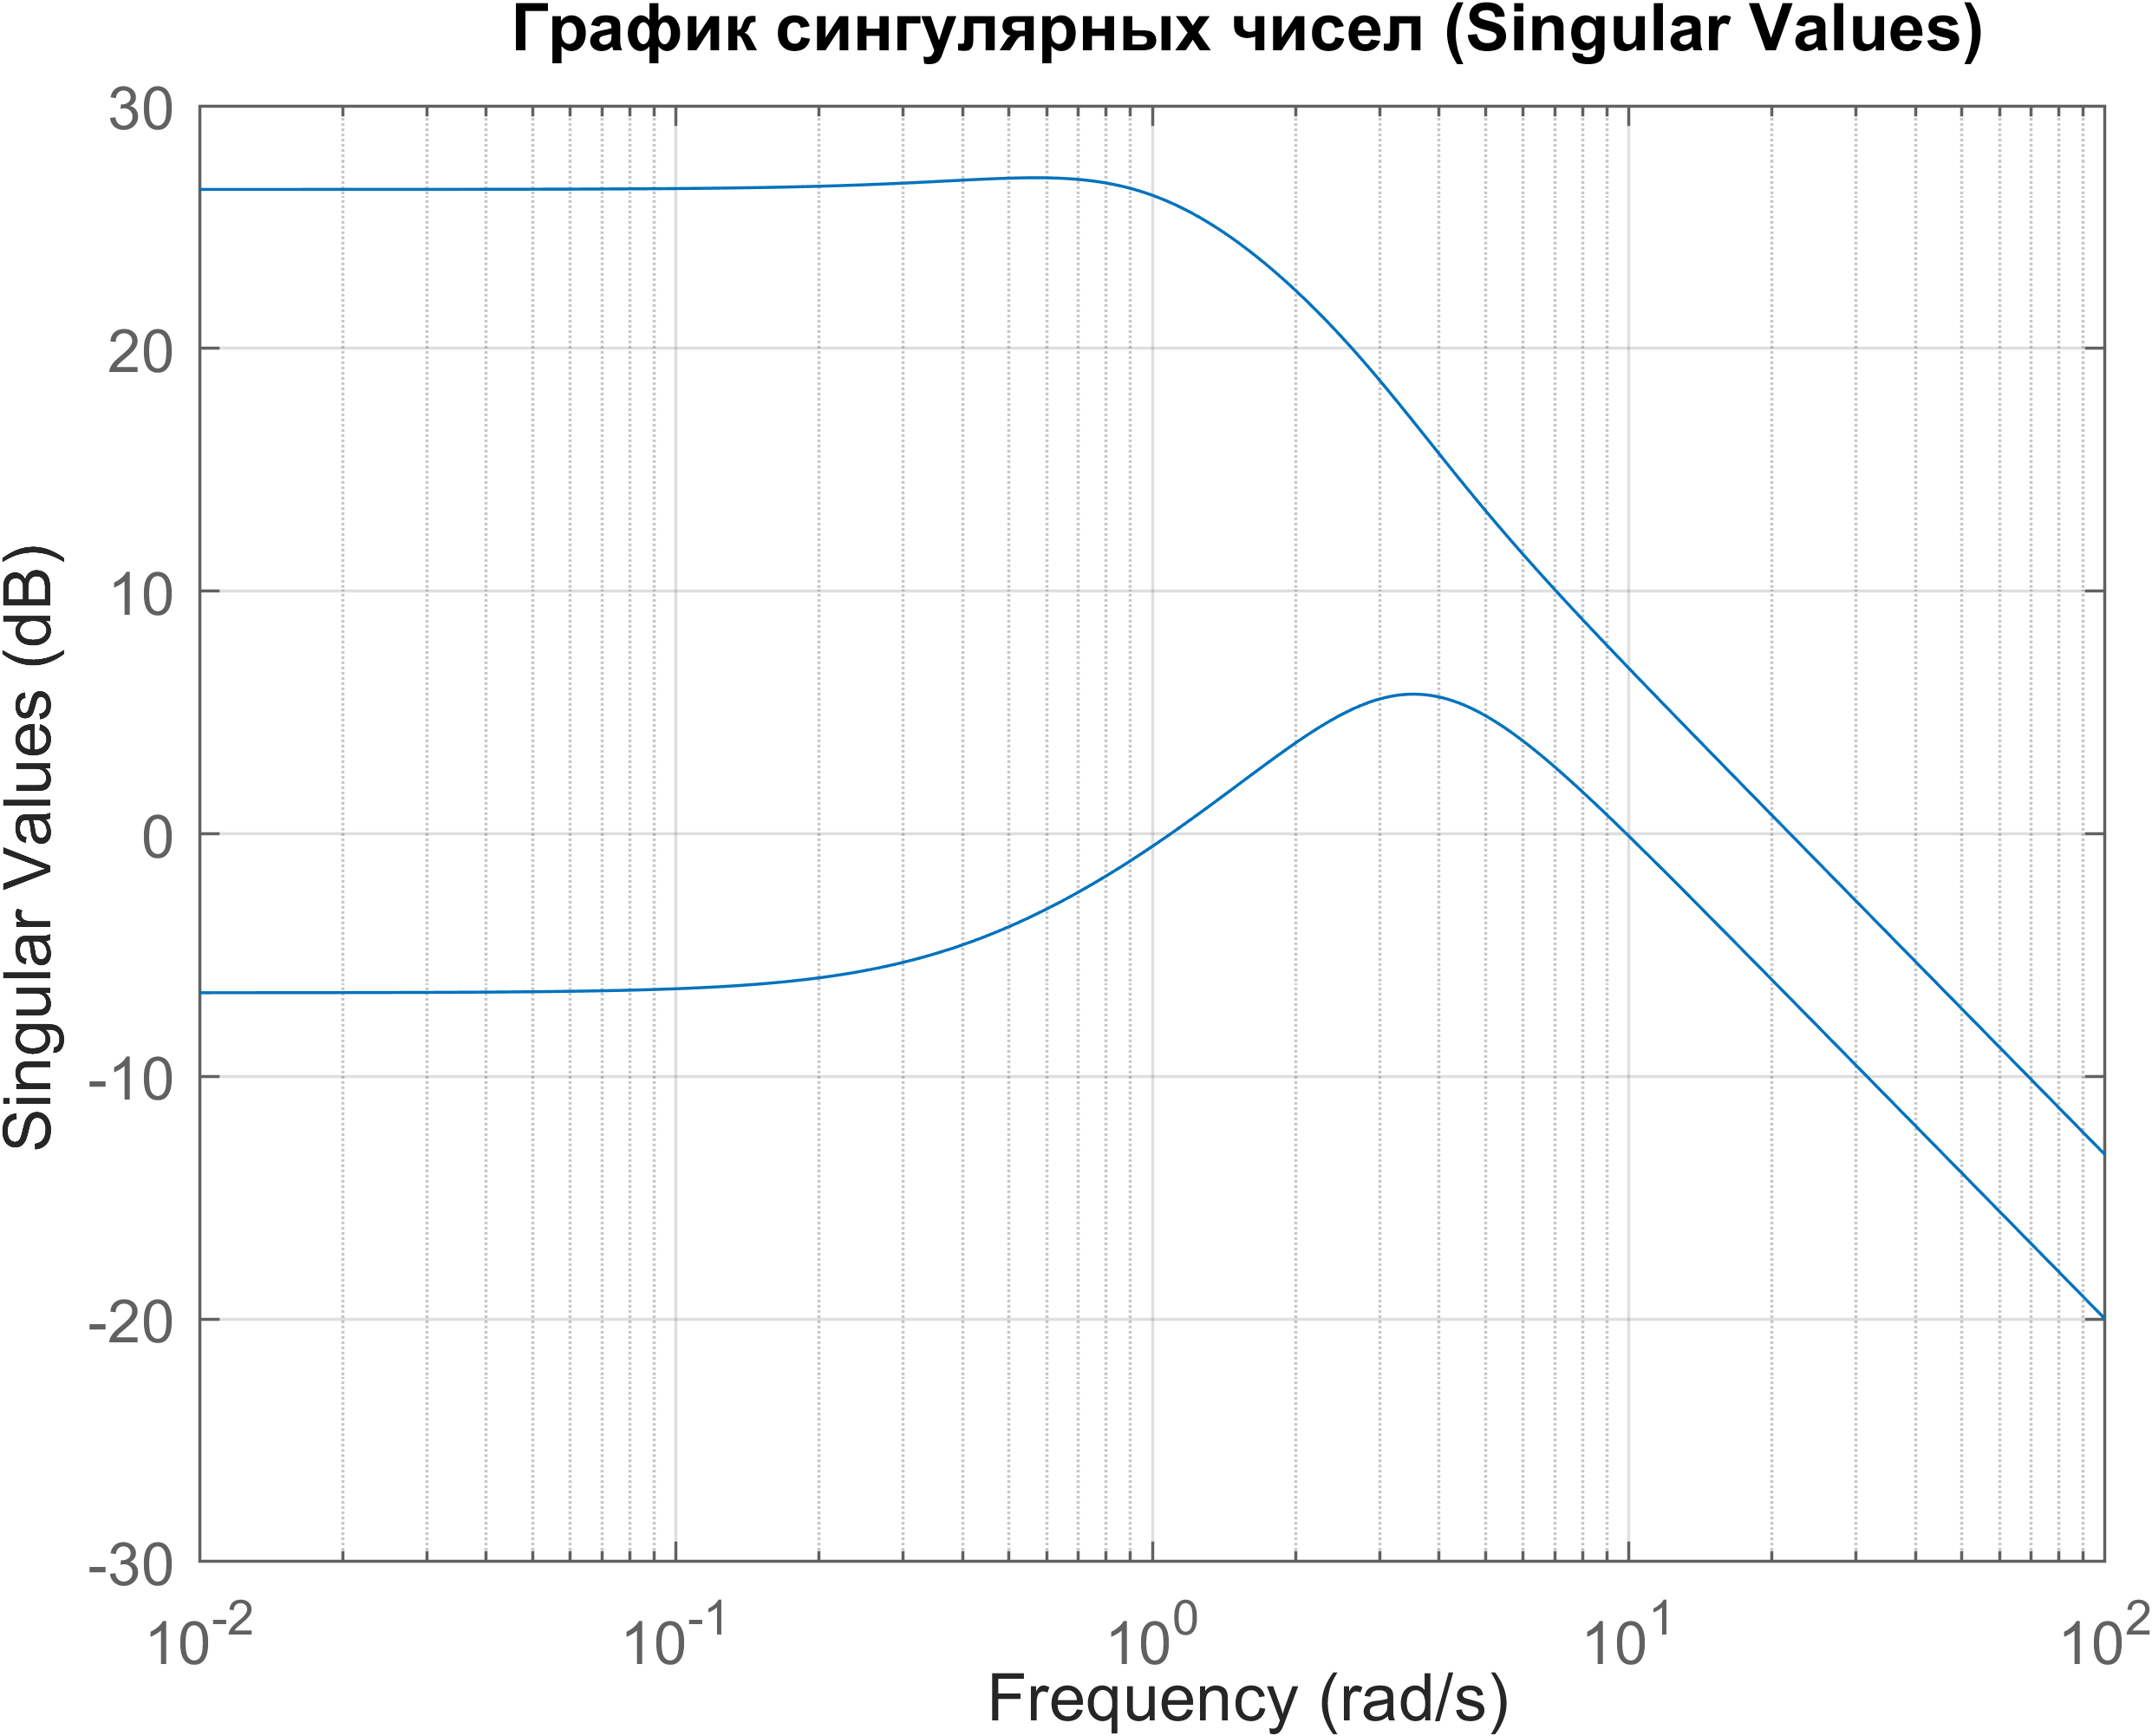
\includegraphics[width=0.7\linewidth]{figs/3_sigma.png}
    \caption{Сингулярные числа $\underset{w\rightarrow z}{W}(s)$}
    \label{fig:3sigma}
\end{figure}
\noindent Найдем нормы $\underset{w\rightarrow z}{W}(s)$:
\begin{equation*}
    ||\underset{w\rightarrow z}{W}(s)||_{H2}=32.2654,\quad
    ||\underset{w\rightarrow z}{W}(s)||_{H\infty}=183.5281.
\end{equation*}
Как видно из графика сингулярных чисел, наихудшая частота возмущения $1.5$.
Таким образом, зададимся двумя возмущениями:
\begin{equation*}
    w_1(t)=\begin{bmatrix}
        sin(1.5t)\\
        0
    \end{bmatrix},\quad
    w_2(t)=\begin{bmatrix}
        sin(10t)\\
        0
    \end{bmatrix}.
\end{equation*}
\begin{figure}[H]
    \centering
    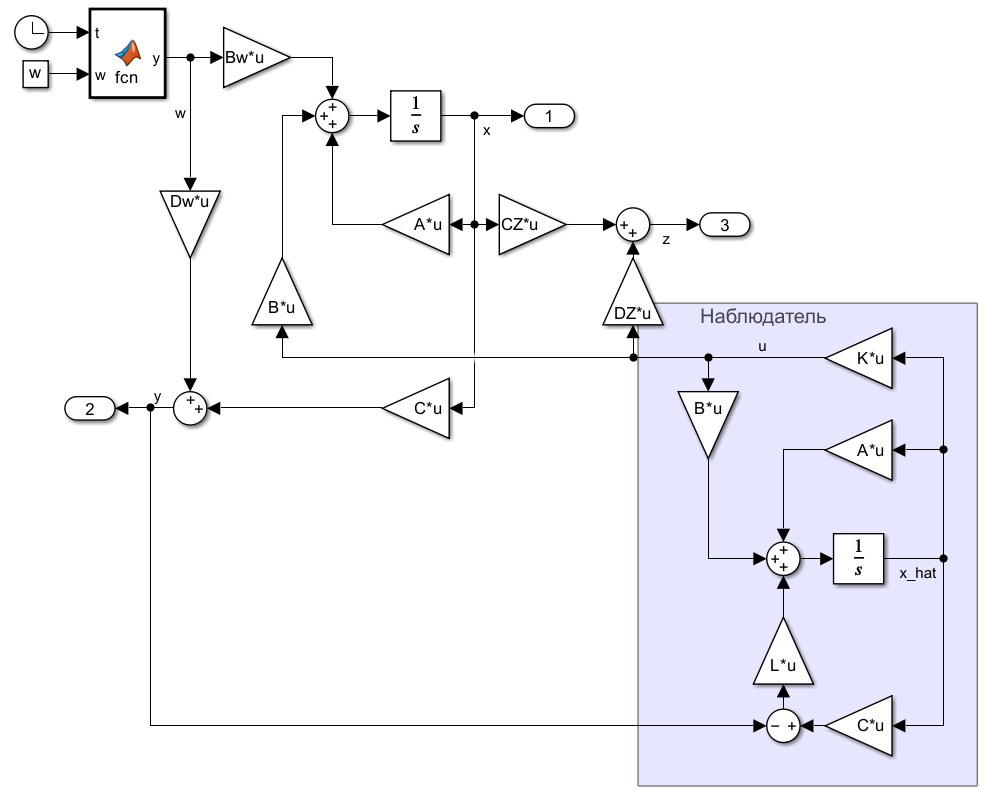
\includegraphics[width=1\linewidth]{figs/3_slx.png}
    \caption{Структурная схема системы \eqref{eq:sys} с наблюдателем в SIMULINK}
    \label{fig:3slx}
\end{figure}
С помощью SIMULINK (см. \autoref{fig:3slx}) для каждого из выбранных вариантов внешнего возмущения $w$ выполним 
компьютерное моделирование замкнутой системы при нулевых начальных условиях
на объекте управления и наблюдателе и построим графики компонент регулируемого выхода
$z(t)$, которые можно увидеть на \autoref{fig:3sim}.
\begin{figure}[H]
    \centering
    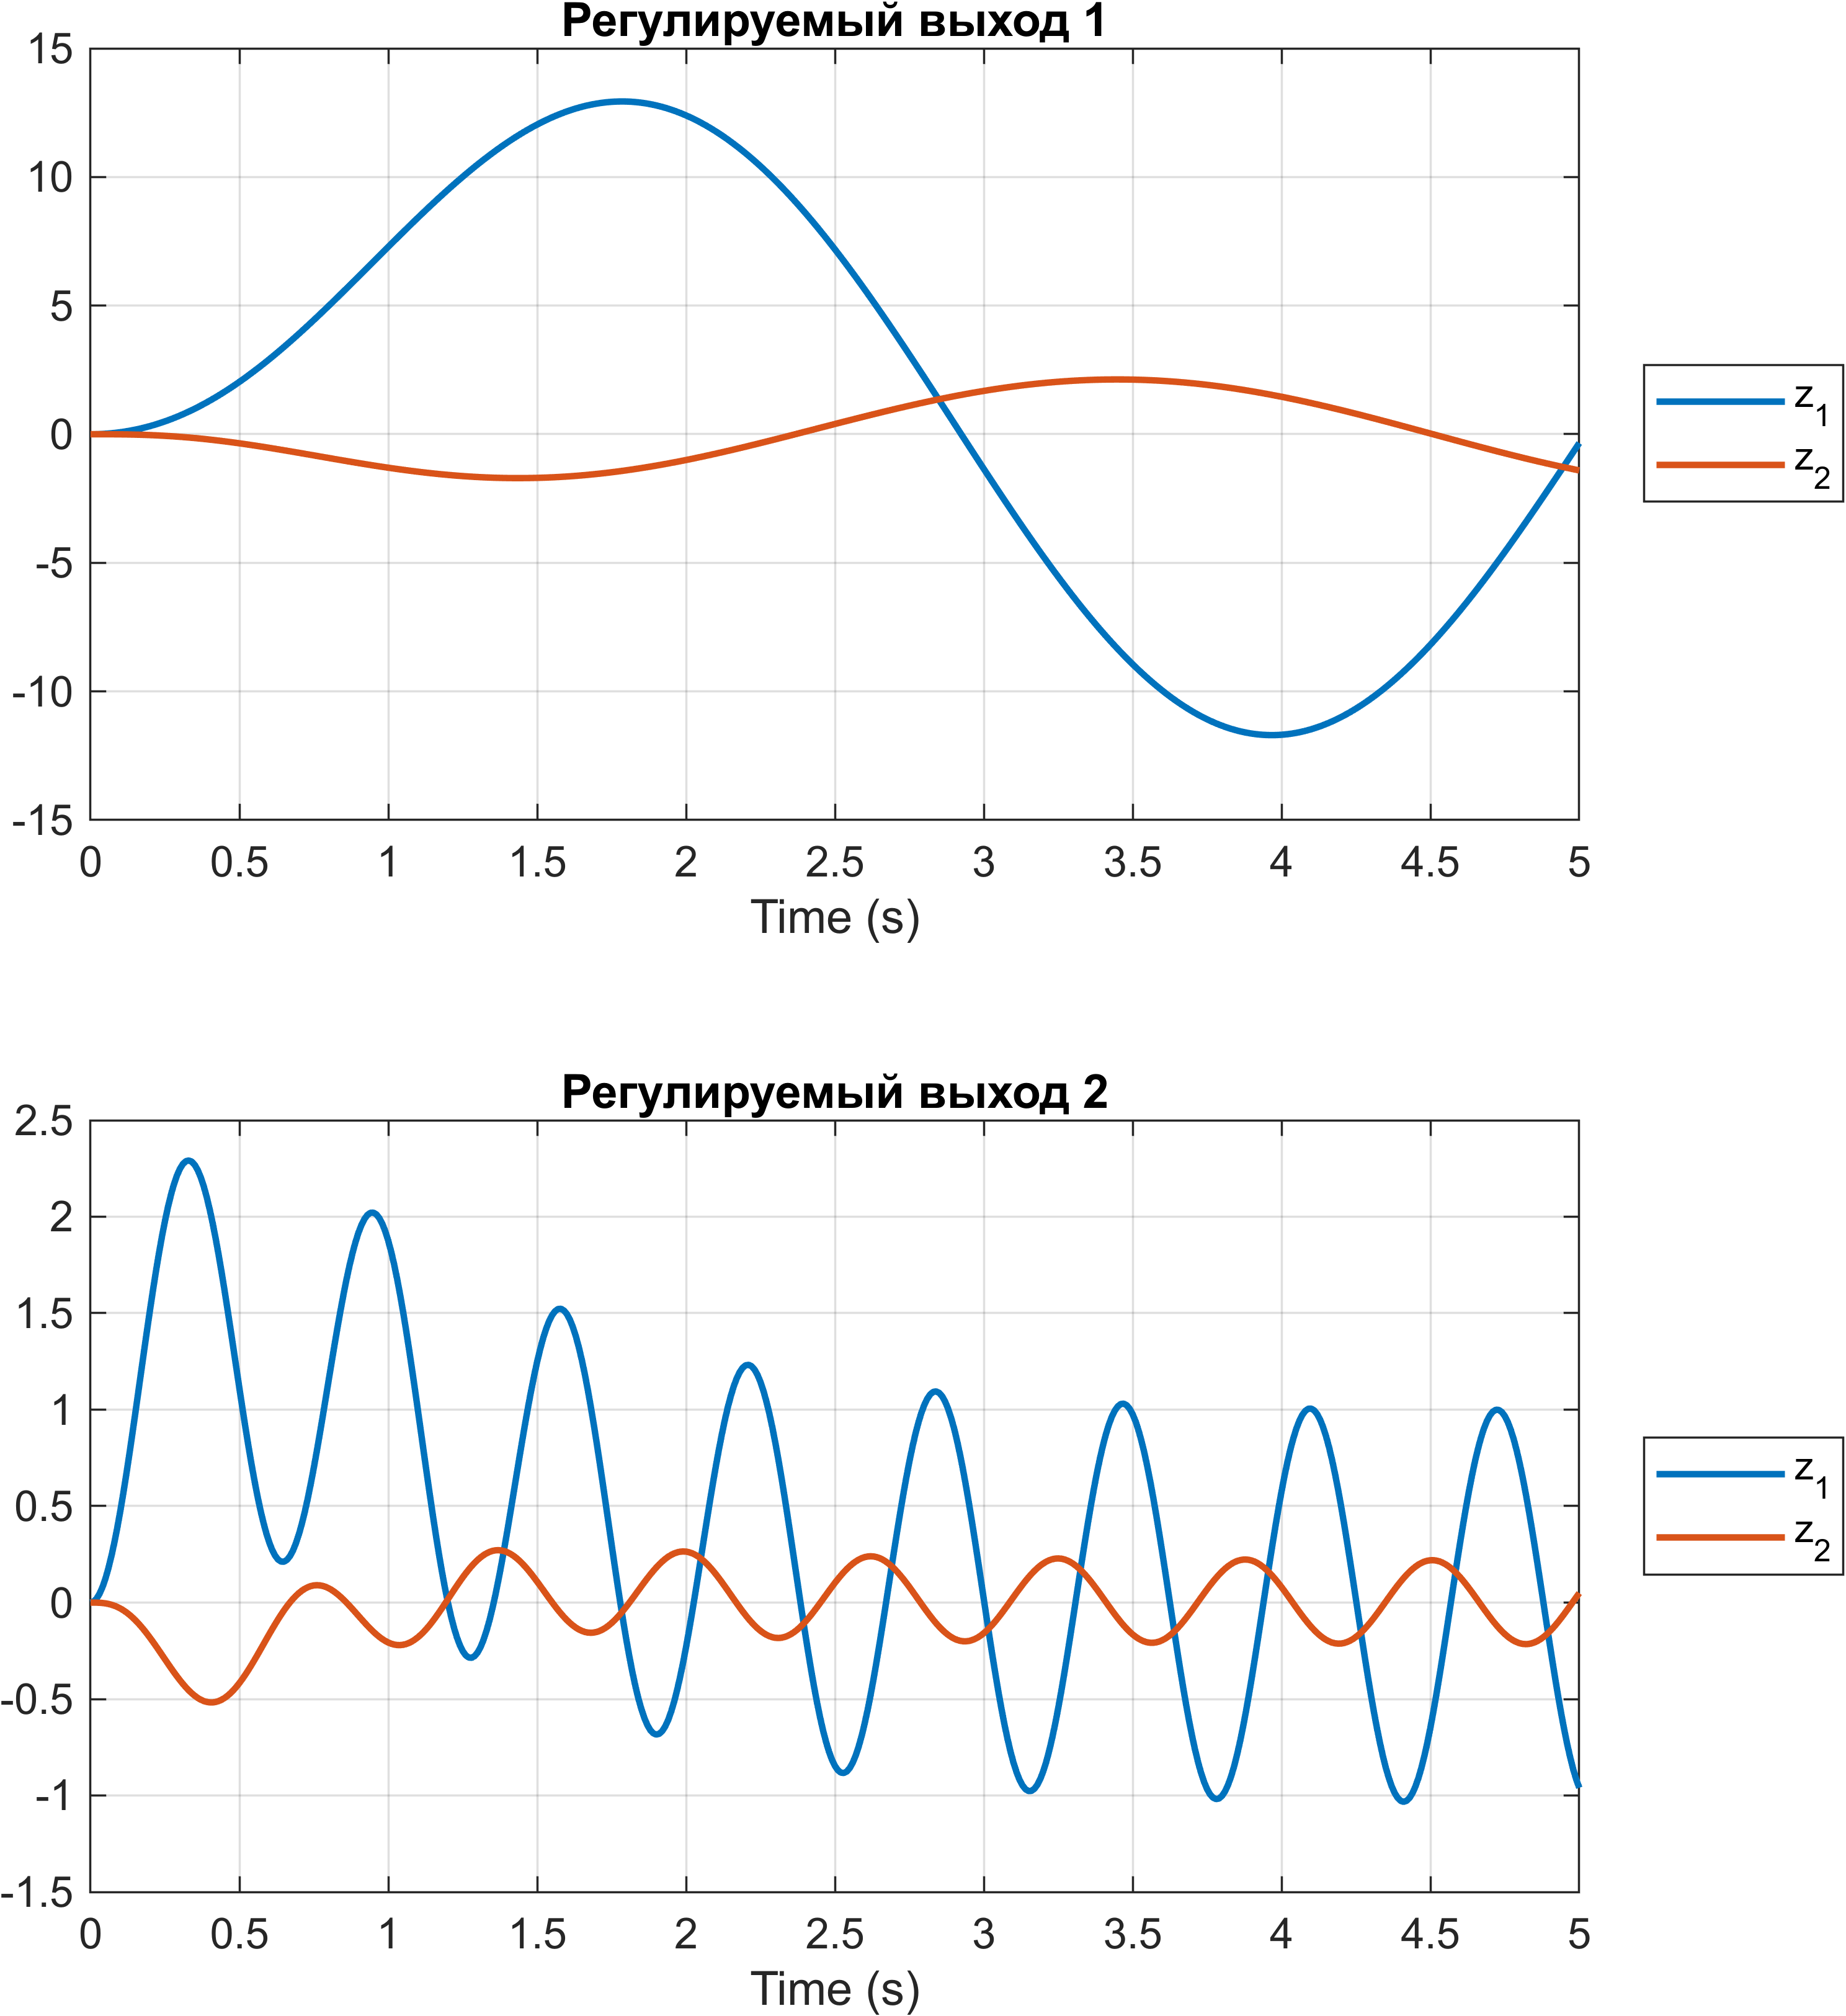
\includegraphics[width=1\linewidth]{figs/3_sim.png}
    \caption{График $z(t)$ при $w_1(t)$ и $w_2(t)$}
    \label{fig:3sim}
\end{figure}

\subsubsection{Выводы}

Из графиков видно, что полностью побороть помеху не удалось, что естественно, и регулируемый выход 
колеблется около нуля. Также видно, что на 
частоте 1.5 амплитуда колебаний  в несколько больше чем для 10.


\subsection{Второй вариант регулируемого выхода}

Так как при построении H2-регулятора по выходу действует separation principle,
в качестве $K$ возьмем матрицу из \autoref{sec:regout2}:
\begin{equation*}
    K=\begin{bmatrix}
        -10.0000&-50.1996
    \end{bmatrix}.
\end{equation*}
Так как матрицы $C_Z$ и $D_Z$ никак не участвуют в синтезе H2-наблюдателя,
матрица $L$ не измениться с предыдущего пункта:
\begin{equation*}
    L=\begin{bmatrix}
        -1.7321 &
        -1.0000
    \end{bmatrix}^T.
\end{equation*}
Передаточная матрица, полученная через tf в MATLAB, замкнутой системы от внешнего возмущения $w$ к выходу $z$:
\begin{equation*}
    \underset{w\rightarrow z}{W}(s)=\begin{bmatrix}
        \underset{w\rightarrow z}{W_1}(s) & \underset{w\rightarrow z}{W_2}(s)\\
        \underset{w\rightarrow z}{W_3}(s) & \underset{w\rightarrow z}{W_4}(s)
    \end{bmatrix},
\end{equation*}
где
\begin{gather*}
    \underset{w\rightarrow z}{W_1}(s)=\dfrac{ 60 s^3 + 3126 s^2 + 3020 s + 479.5}{s^4 + 51.93 s^3 + 97.95 s^2 + 67.52 s + 10}\\
    \underset{w\rightarrow z}{W_2}(s)=\dfrac{ -3376 s^2 - 1175 s - 100}{s^4 + 51.93 s^3 + 97.95 s^2 + 67.52 s + 10}\\
    \underset{w\rightarrow z}{W_3}(s)=\dfrac{  -67.52 s^2 - 77.52 s - 10}{s^4 + 51.93 s^3 + 97.95 s^2 + 67.52 s + 10}\\
    \underset{w\rightarrow z}{W_4}(s)=\dfrac{  -67.52 s^3 - 10 s^2 - 3.245e-15 s - 4.805e-16}{s^4 + 51.93 s^3 + 97.95 s^2 + 67.52 s + 10}
\end{gather*}
График покомпонентных АЧХ $\underset{w\rightarrow z}{W}(s)$ представлен на \autoref{fig:4bodemag}.
\begin{figure}[H]
    \centering
    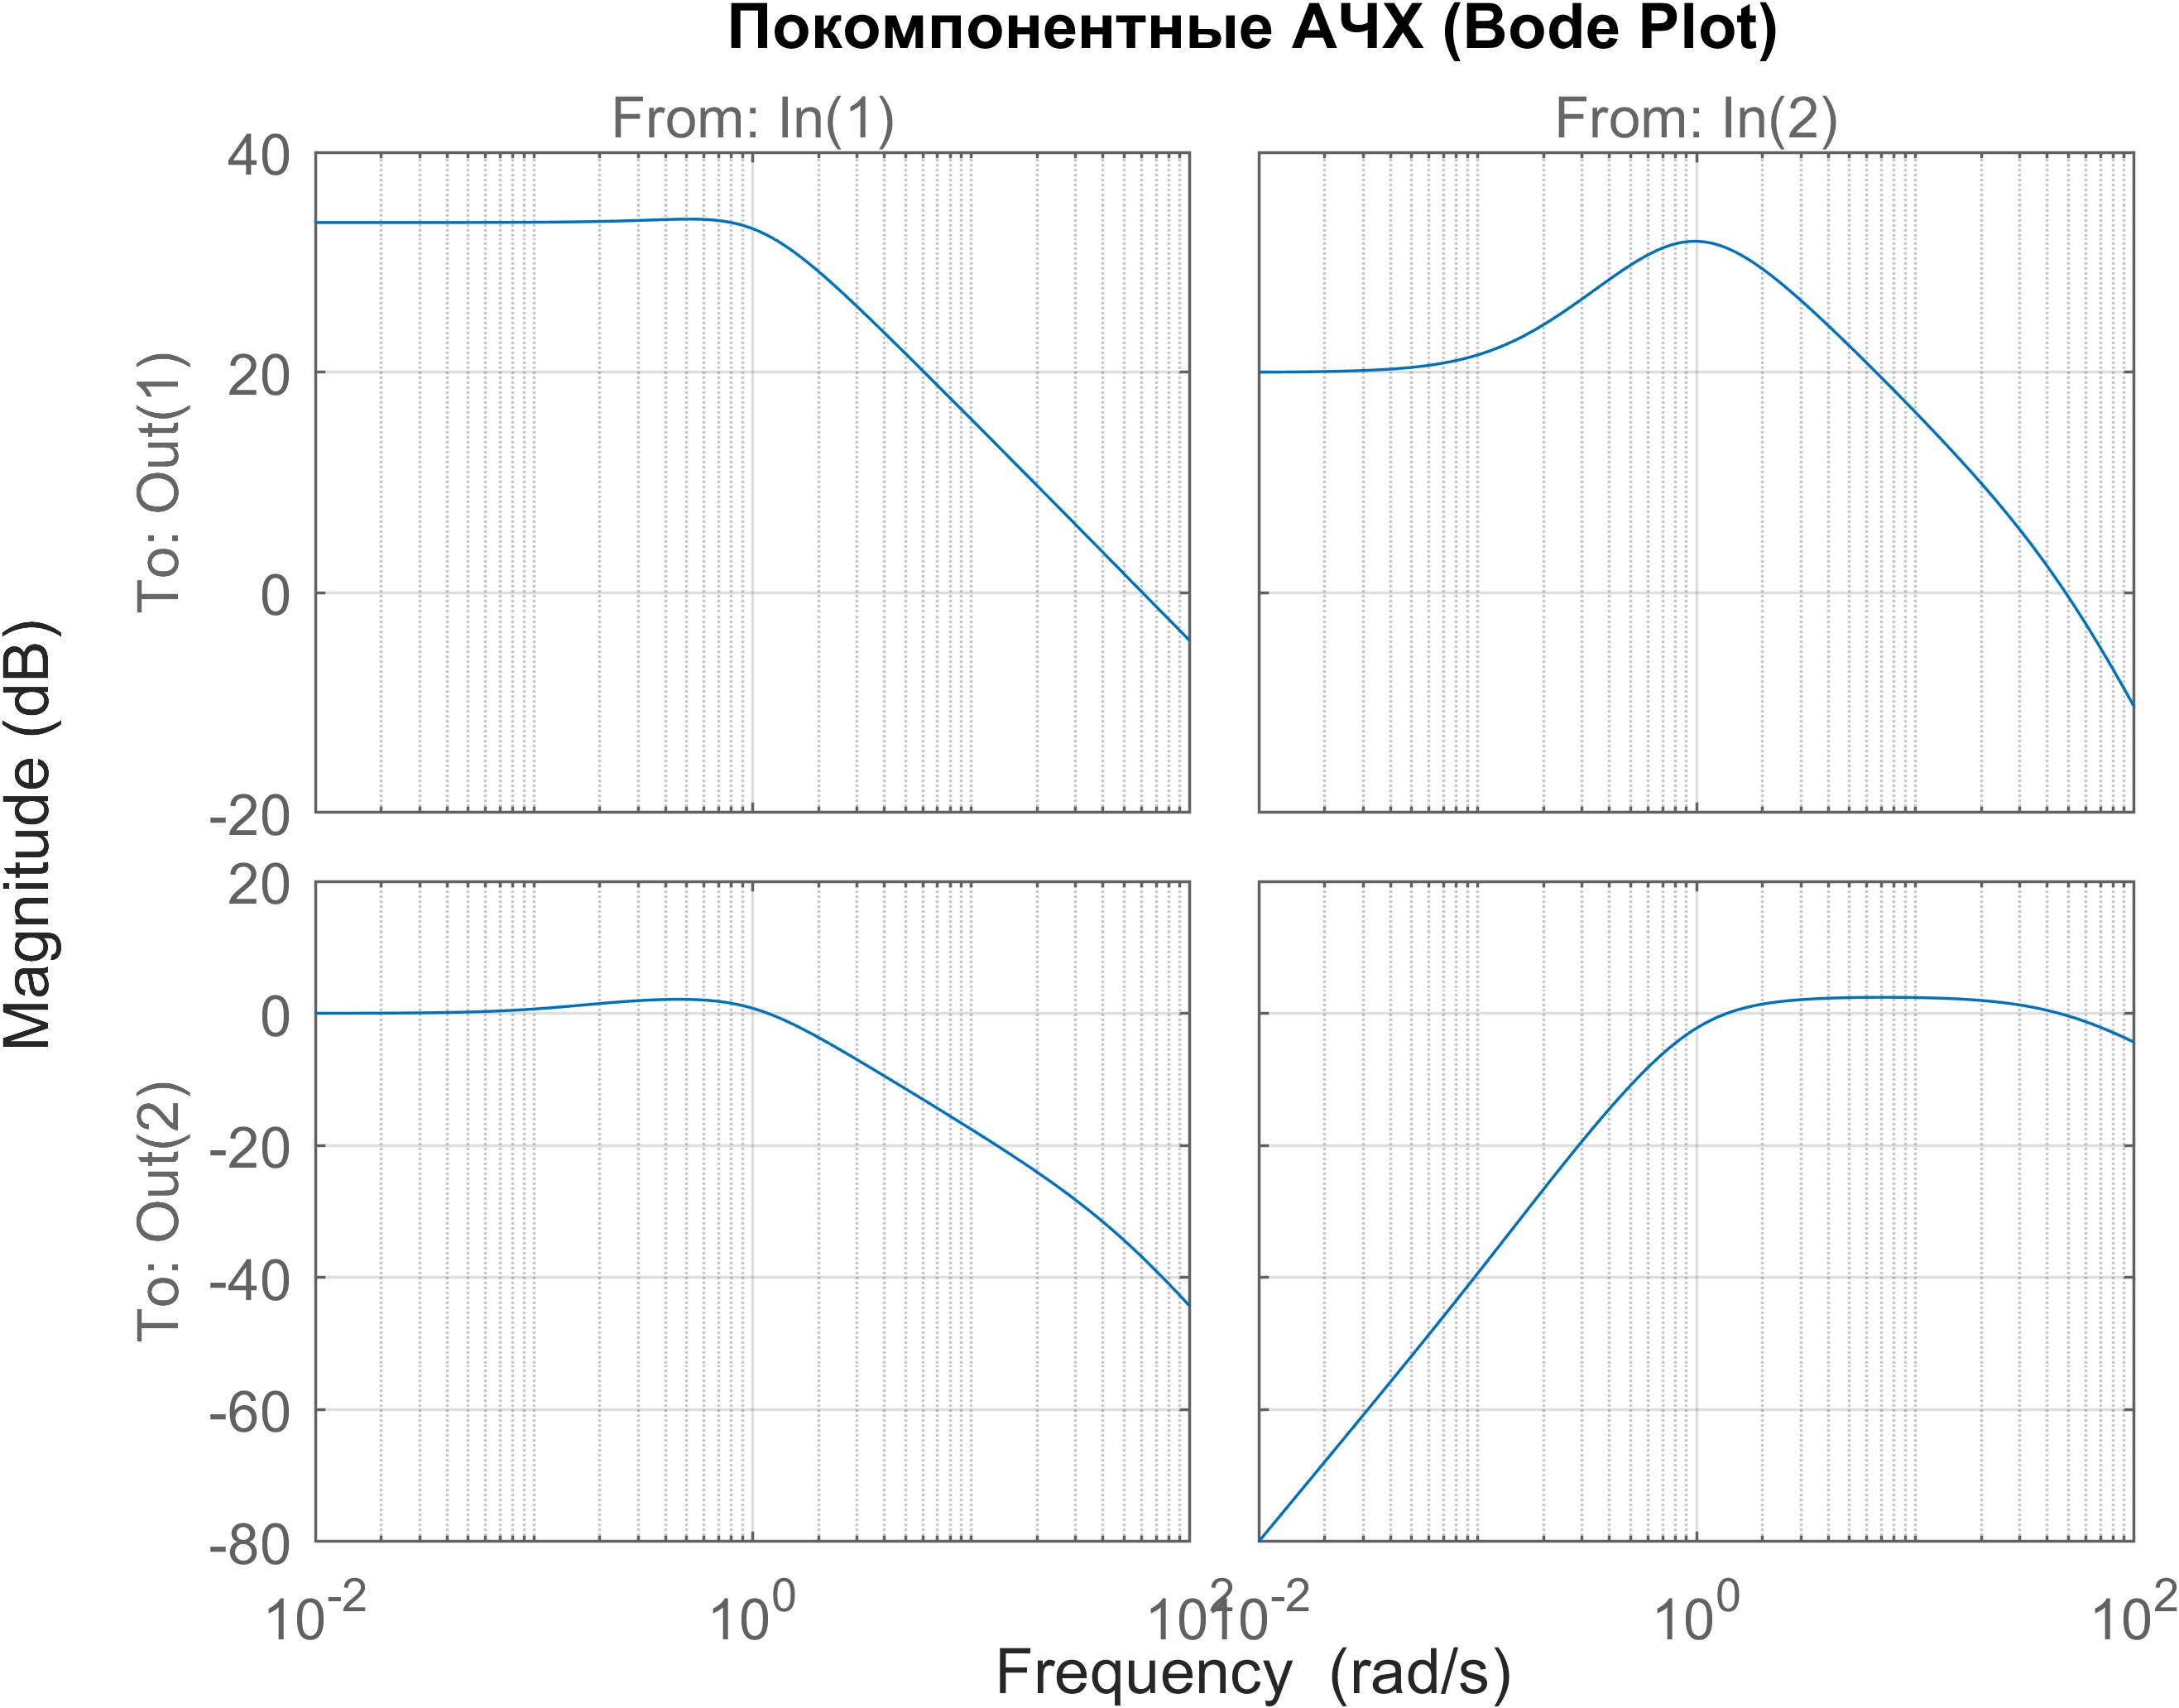
\includegraphics[width=0.7\linewidth]{figs/4_bodemag.png}
    \caption{Покомпонентные АЧХ $\underset{w\rightarrow z}{W}(s)$}
    \label{fig:4bodemag}
\end{figure}
График сингулярных чисел $\underset{w\rightarrow z}{W}(s)$ представлен на \autoref{fig:4sigma}.
\begin{figure}[H]
    \centering
    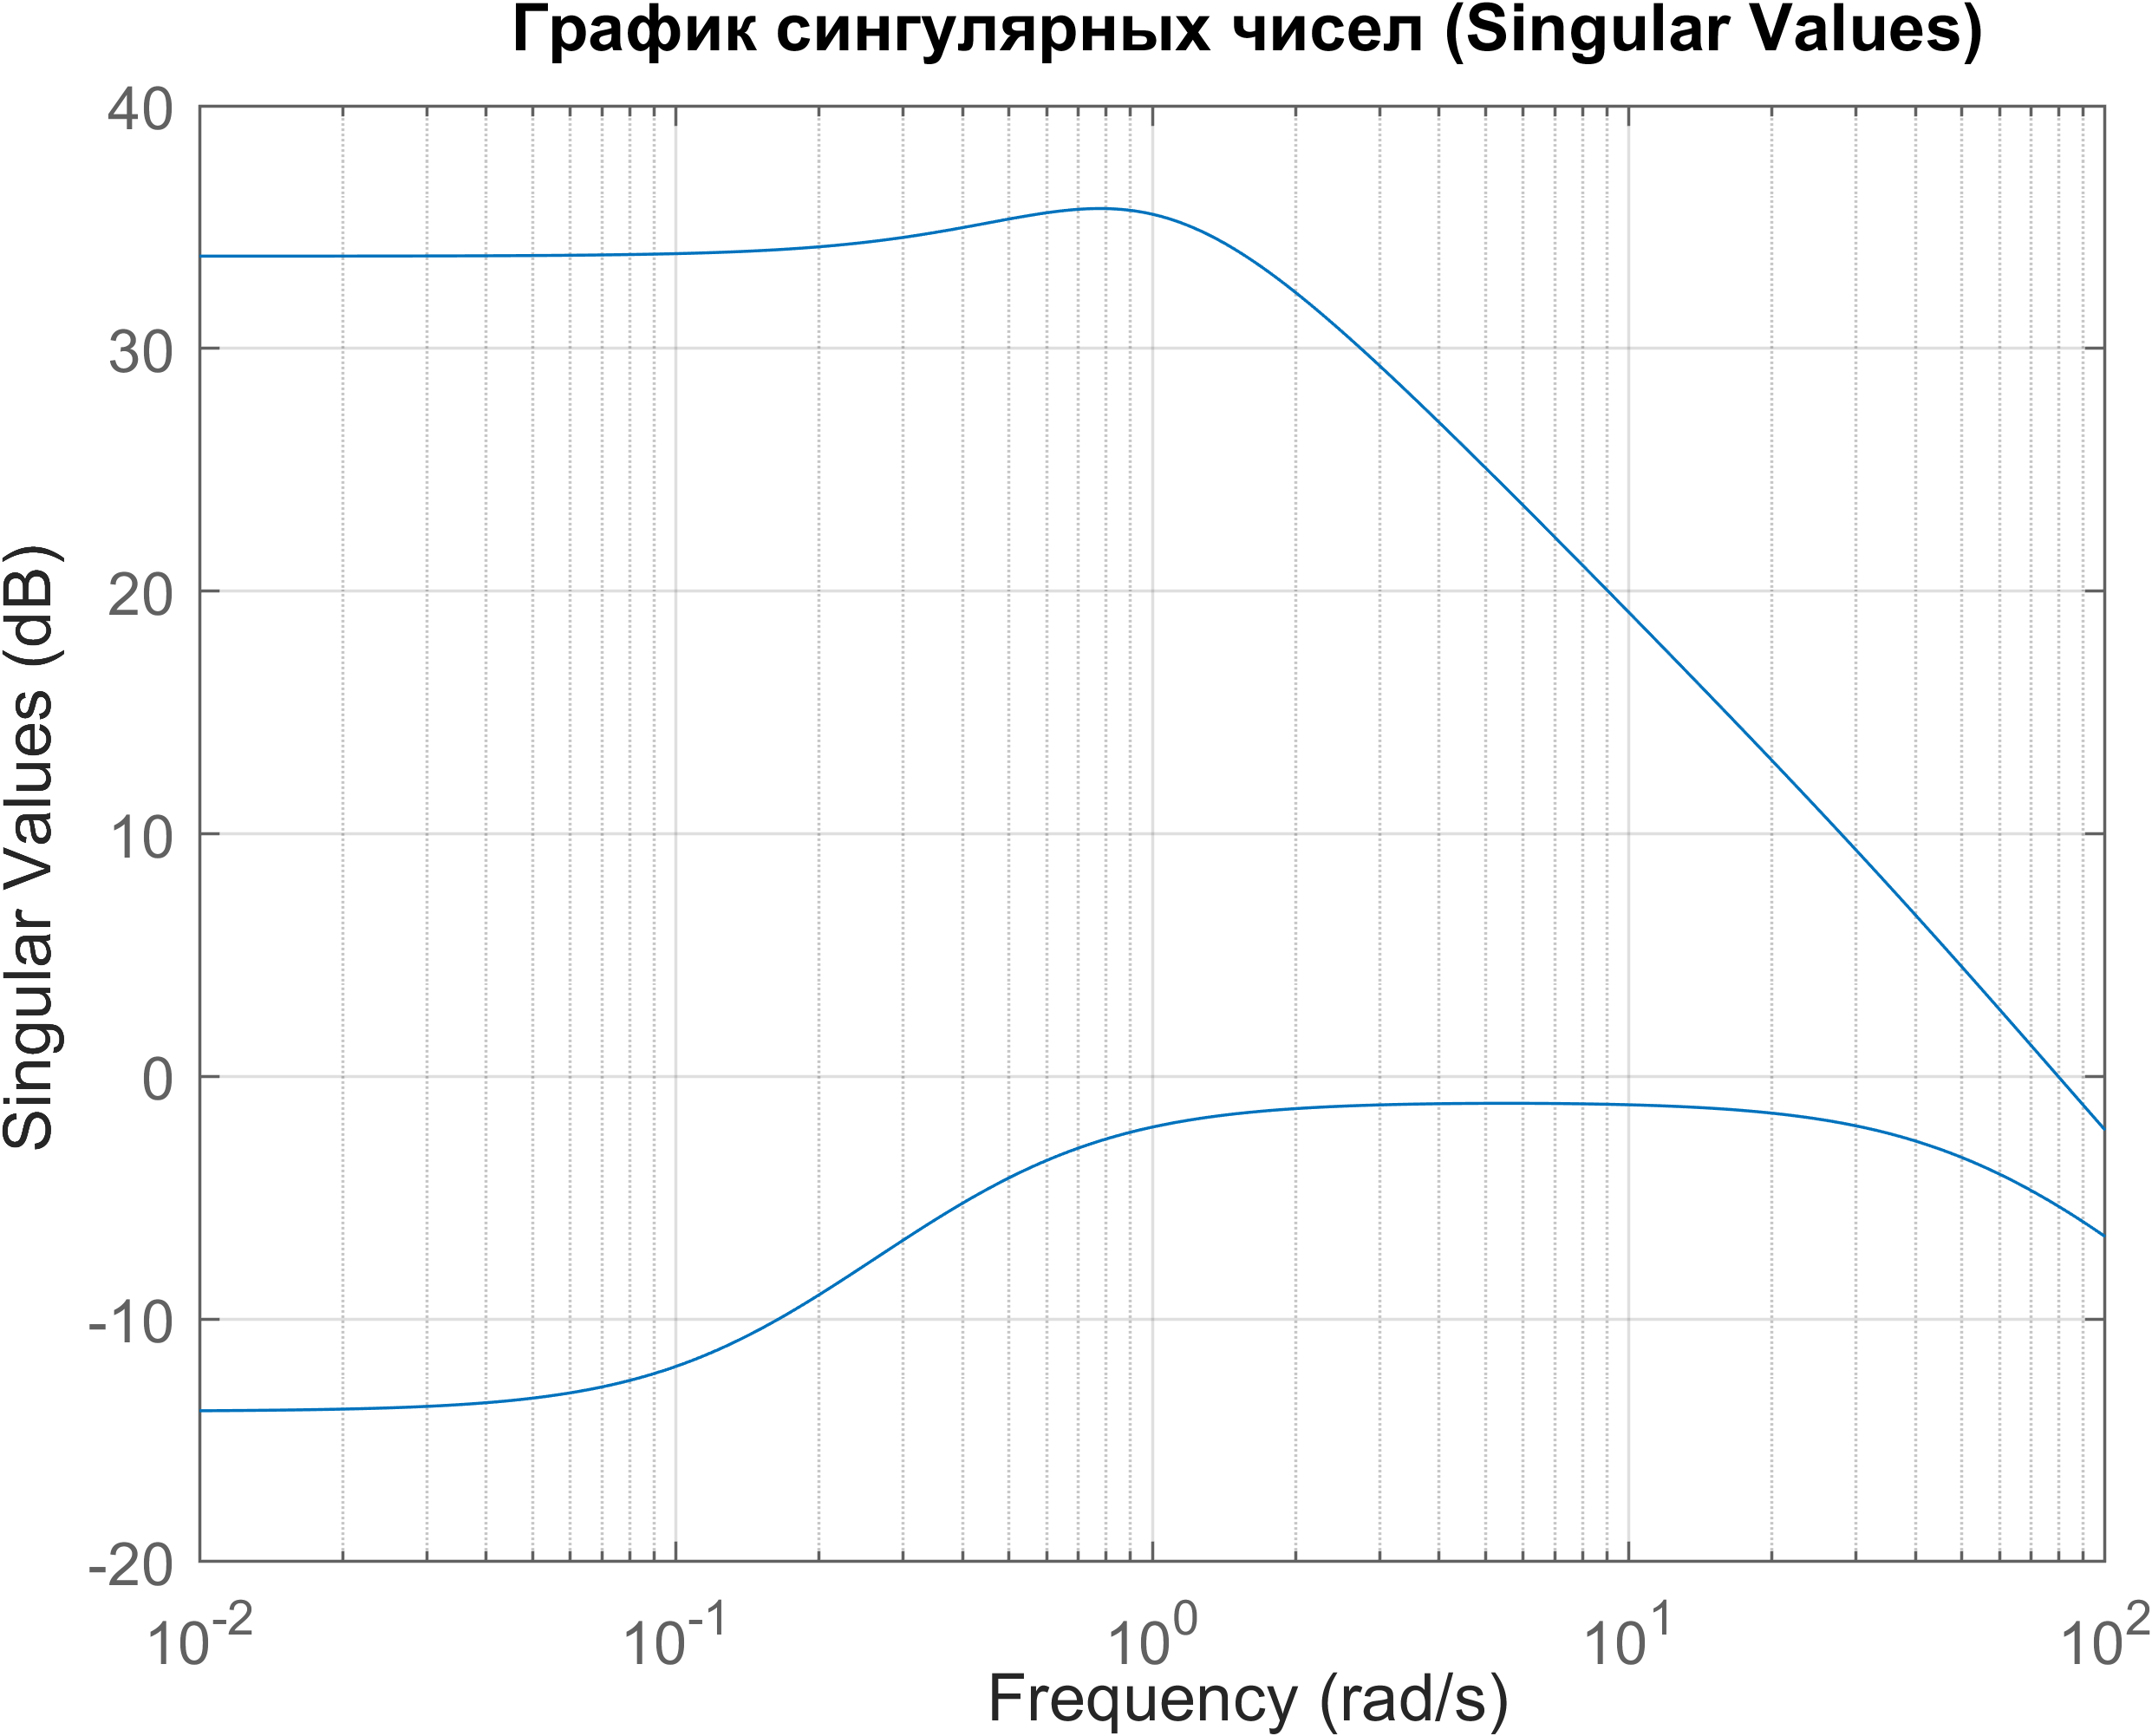
\includegraphics[width=0.7\linewidth]{figs/4_sigma.png}
    \caption{Сингулярные числа $\underset{w\rightarrow z}{W}(s)$}
    \label{fig:4sigma}
\end{figure}
\noindent Найдем нормы $\underset{w\rightarrow z}{W}(s)$:
\begin{equation*}
    ||\underset{w\rightarrow z}{W}(s)||_{H2}=55.6252,\quad
    ||\underset{w\rightarrow z}{W}(s)||_{H\infty}=61.4190.
\end{equation*}
Как видно из графика сингулярных чисел, наихудшая частота возмущения $1$.
Таким образом, зададимся двумя возмущениями:
\begin{equation*}
    w_1(t)=\begin{bmatrix}
        sin(t)\\
        0
    \end{bmatrix},\quad
    w_2(t)=\begin{bmatrix}
        sin(100t)\\
        0
    \end{bmatrix}.
\end{equation*}
С помощью SIMULINK (см. \autoref{fig:3slx}) для каждого из выбранных вариантов внешнего возмущения $w$ выполним 
компьютерное моделирование замкнутой системы при нулевых начальных условиях
на объекте управления и наблюдателе и построим графики компонент регулируемого выхода
$z(t)$, которые можно увидеть на \autoref{fig:4sim}.
\begin{figure}[H]
    \centering
    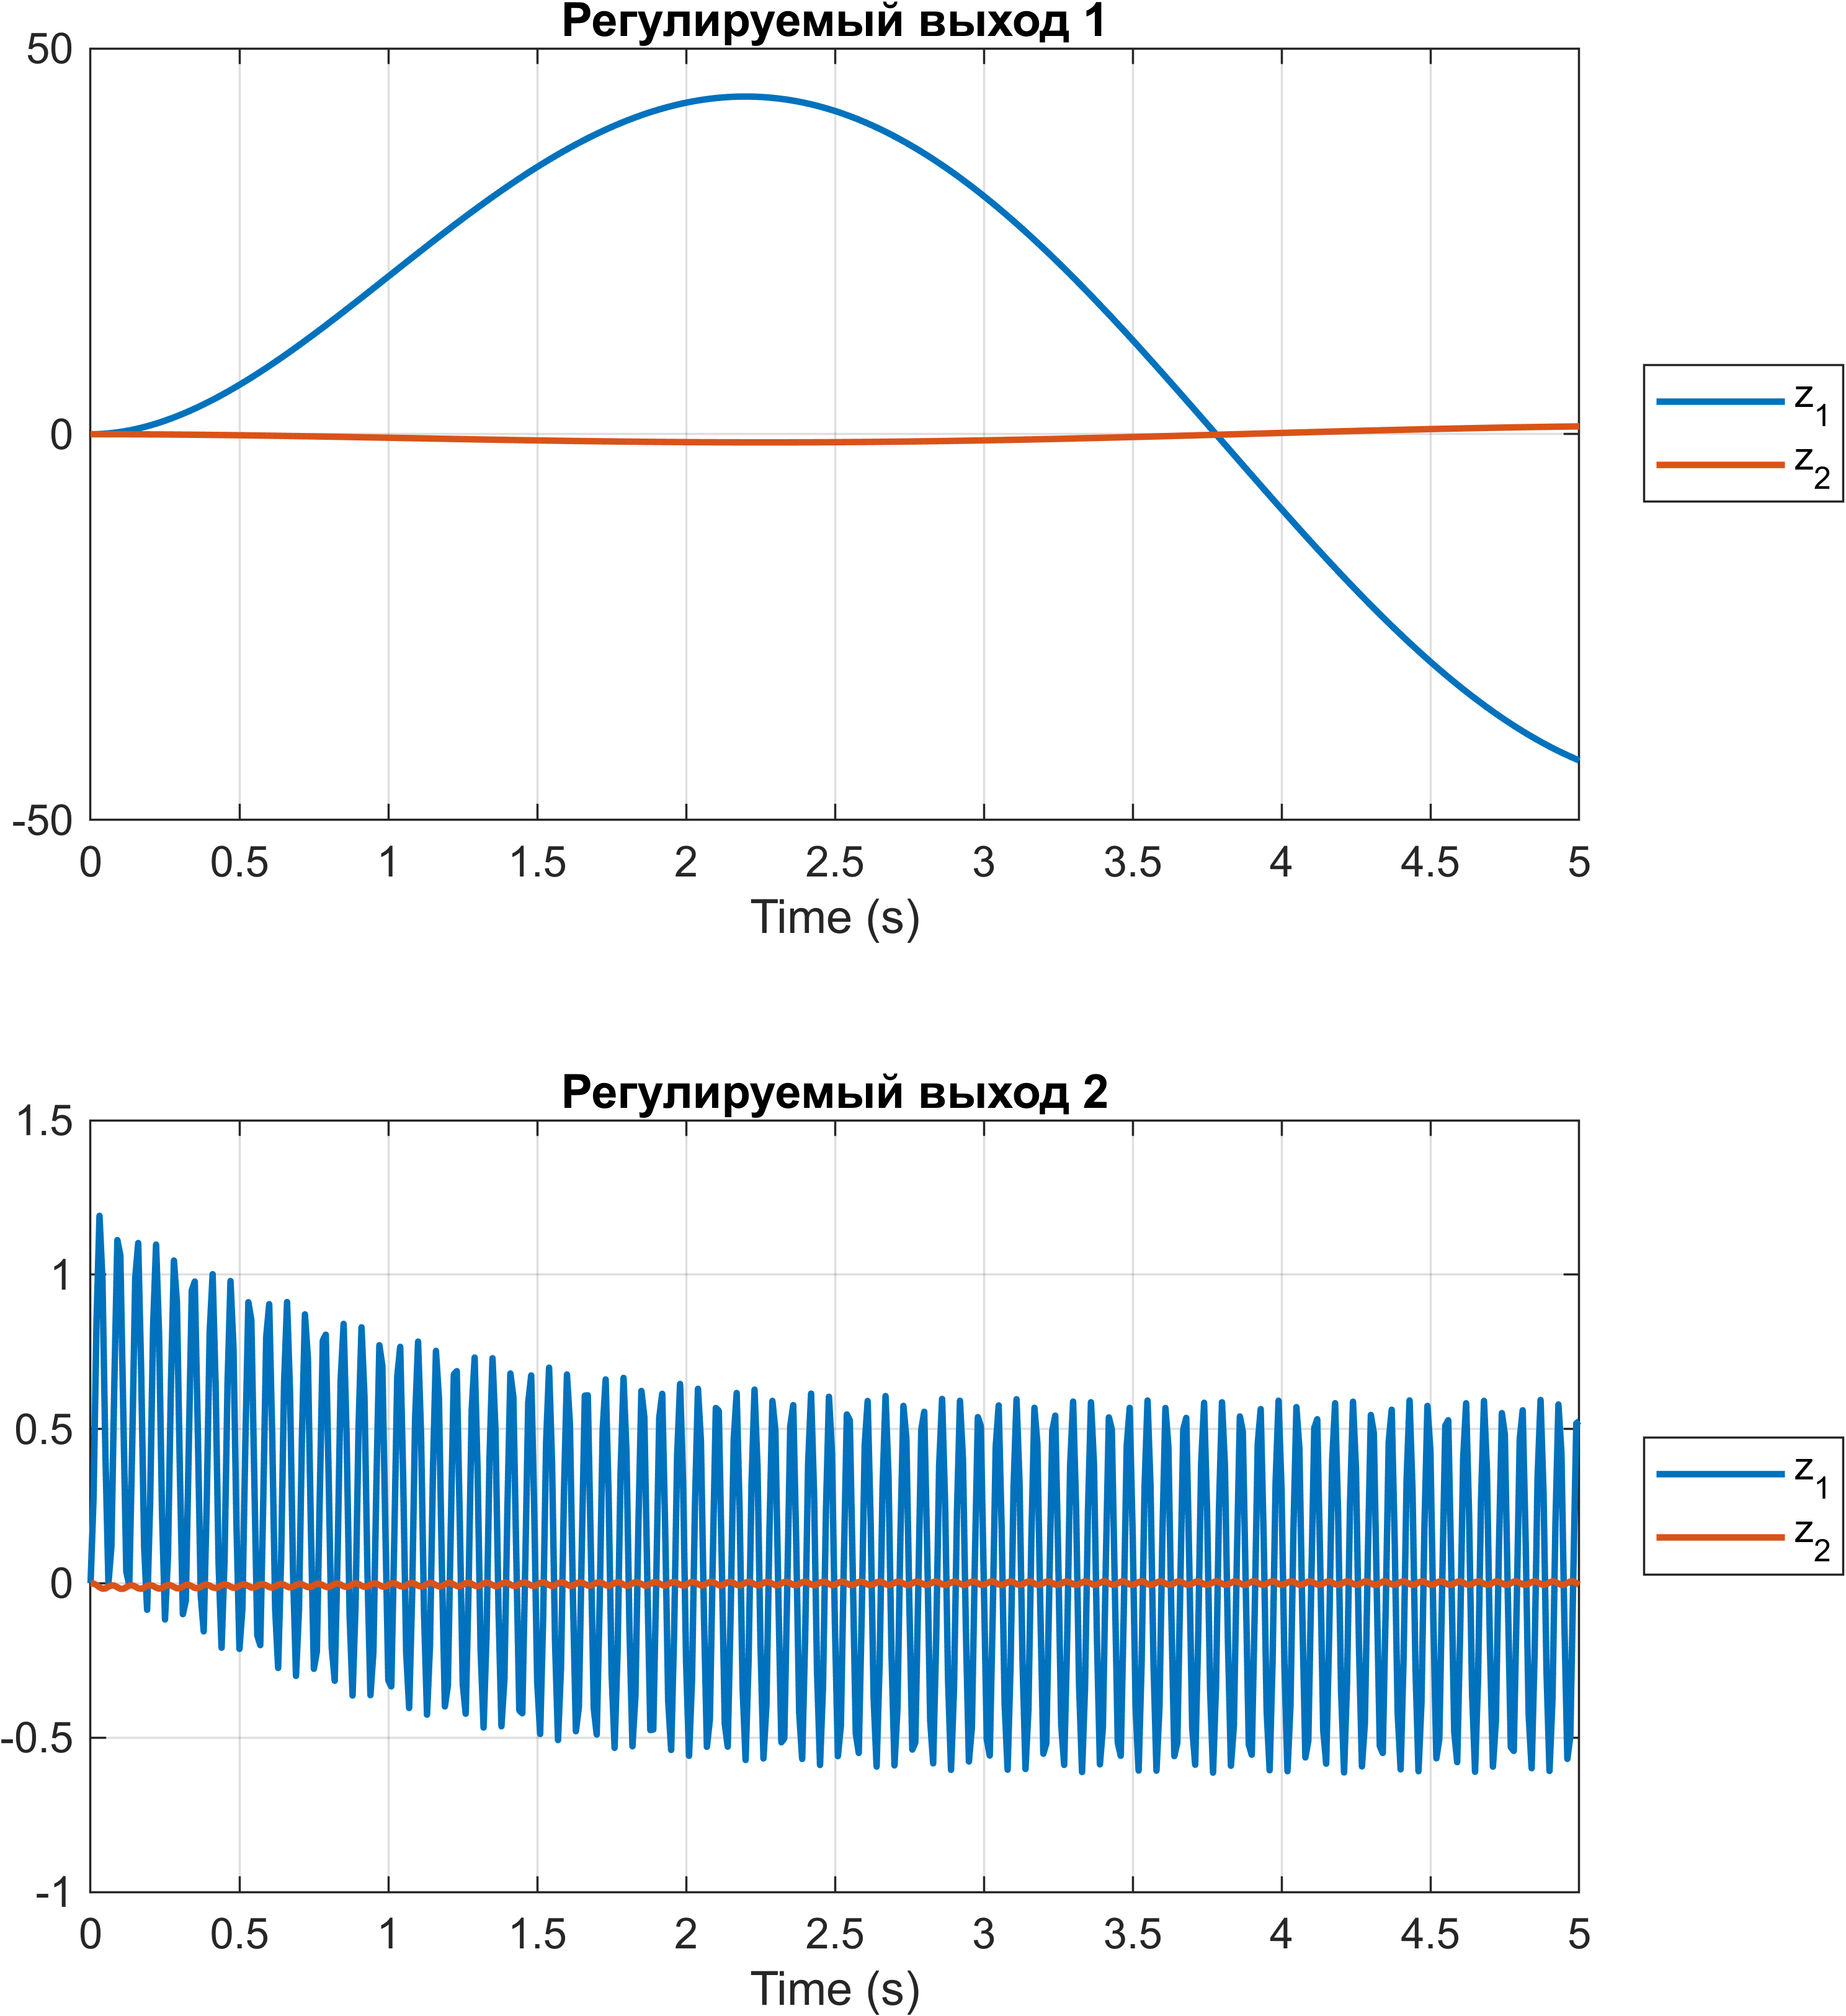
\includegraphics[width=1\linewidth]{figs/4_sim.png}
    \caption{График $z(t)$ при $w_1(t)$ и $w_2(t)$}
    \label{fig:4sim}
\end{figure}

\subsubsection{Выводы}

Из графиков видно, что полностью побороть помеху не удалось, что естественно, и регулируемый выход 
колеблется около нуля. Также видно, что на 
частоте 1 амплитуда колебаний  в несколько больше чем для 100.



\section{Синтез H infinity регулятора по состоянию}

Будем использовать ($C_{Z1},\ D_{Z1}$) матрицы для регулируемого выхода, и обозначать
без цифр ($C_{Z},\ D_{Z}$). 

\subsection{Минимальная гамма}

Синтезируем H infinity регулятор вида $u=Kx$ по состоянию путем решения матричного
уравнения Риккати:
\begin{equation}
    \label{eq:ric3}
    A^TQ+QA+C_Z^TC_Z-QB(D_Z^TD_Z)^{-1}B^TQ+\gamma^{-2}QB_wB_w^TQ=0,\quad K=-(D_Z^TD_Z)^{-1}B^TQ.
\end{equation}
Используя \texttt{icare} получим
\begin{equation*}
    K=\begin{bmatrix}
        -505.8604	&-184.4152
    \end{bmatrix}.
\end{equation*}
Данная матрица была получена при минимальном $\gamma=3.8$.
Передаточная матрица замкнутой системы от внешнего возмущения $w$ к выходу $z$:
\begin{equation*}
    \underset{w\rightarrow z}{W}(s)=\begin{bmatrix}
        \dfrac{10 s + 1854}{s^2 + 184.4 s + 505.9} & 0 \\[2ex]
        \dfrac{-690.3 s - 505.9}{s^2 + 184.4 s + 505.9} & 0
    \end{bmatrix}
\end{equation*}
График покомпонентных АЧХ $\underset{w\rightarrow z}{W}(s)$ представлен на \autoref{fig:5bodemag}.
\begin{figure}[H]
    \centering
    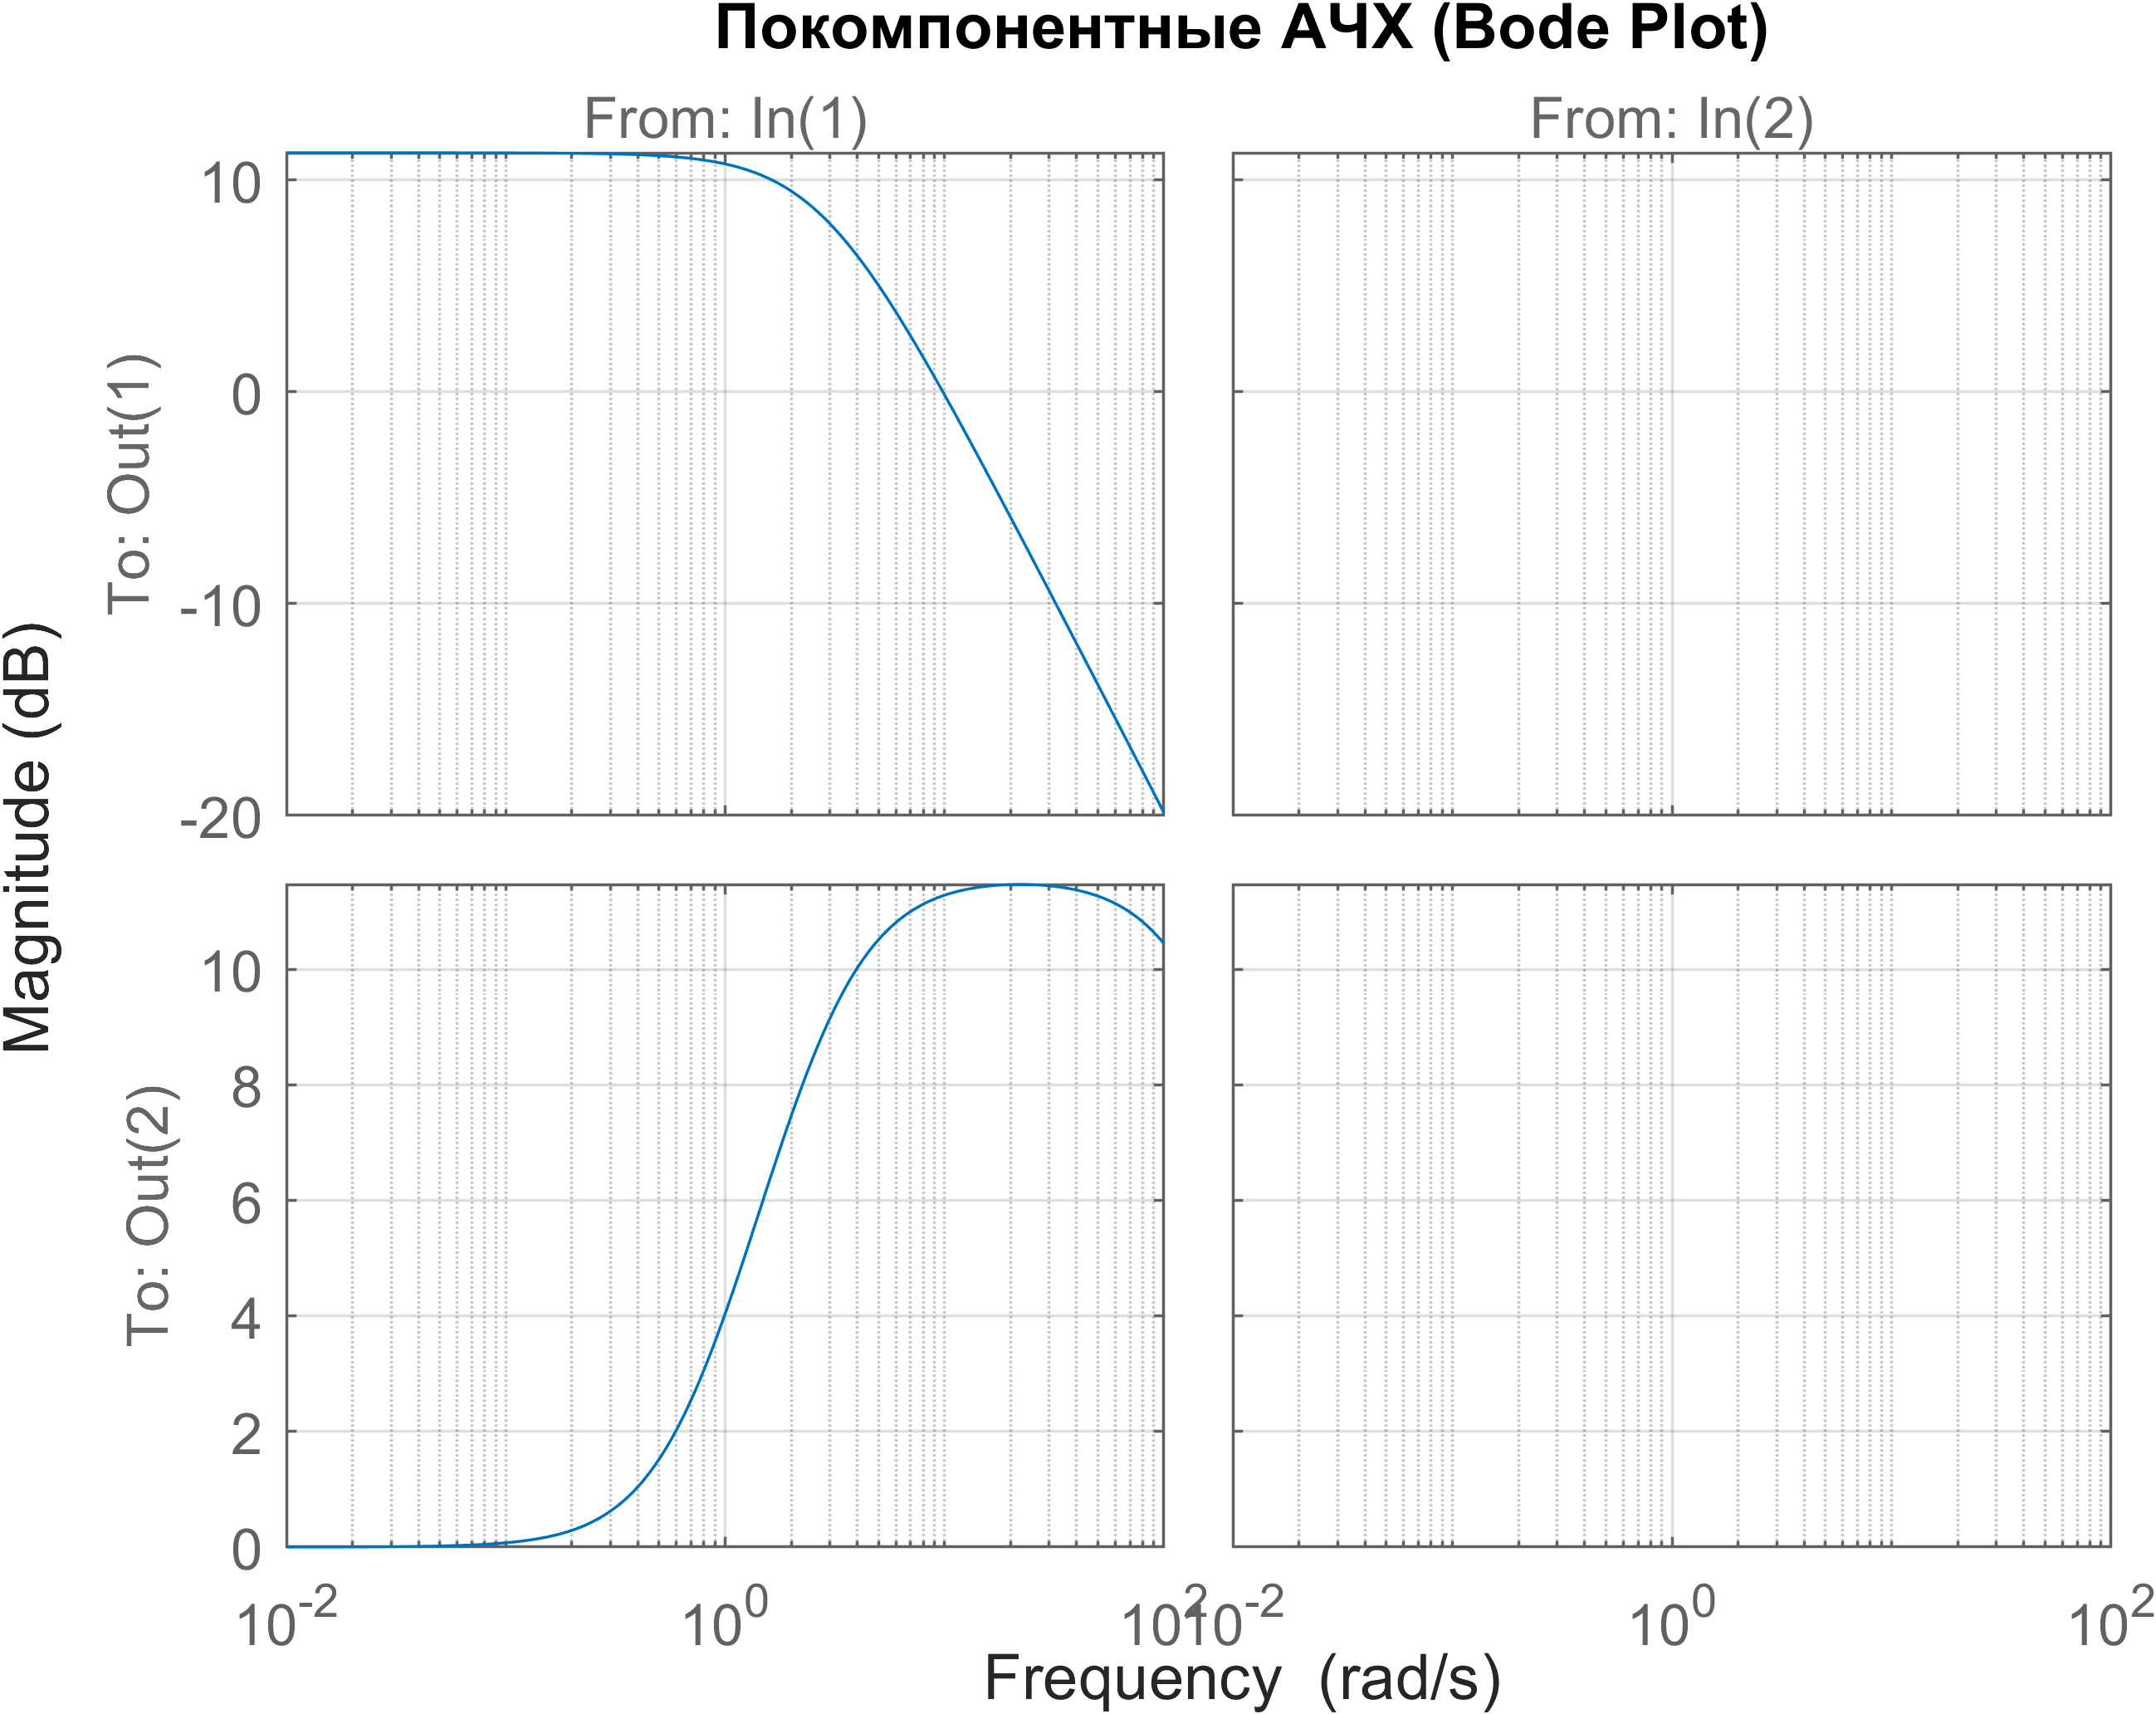
\includegraphics[width=0.8\linewidth]{figs/5_bodemag.png}
    \caption{Покомпонентные АЧХ $\underset{w\rightarrow z}{W}(s)$}
    \label{fig:5bodemag}
\end{figure}
График сингулярных чисел $\underset{w\rightarrow z}{W}(s)$ представлен на \autoref{fig:5sigma}.
\begin{figure}[H]
    \centering
    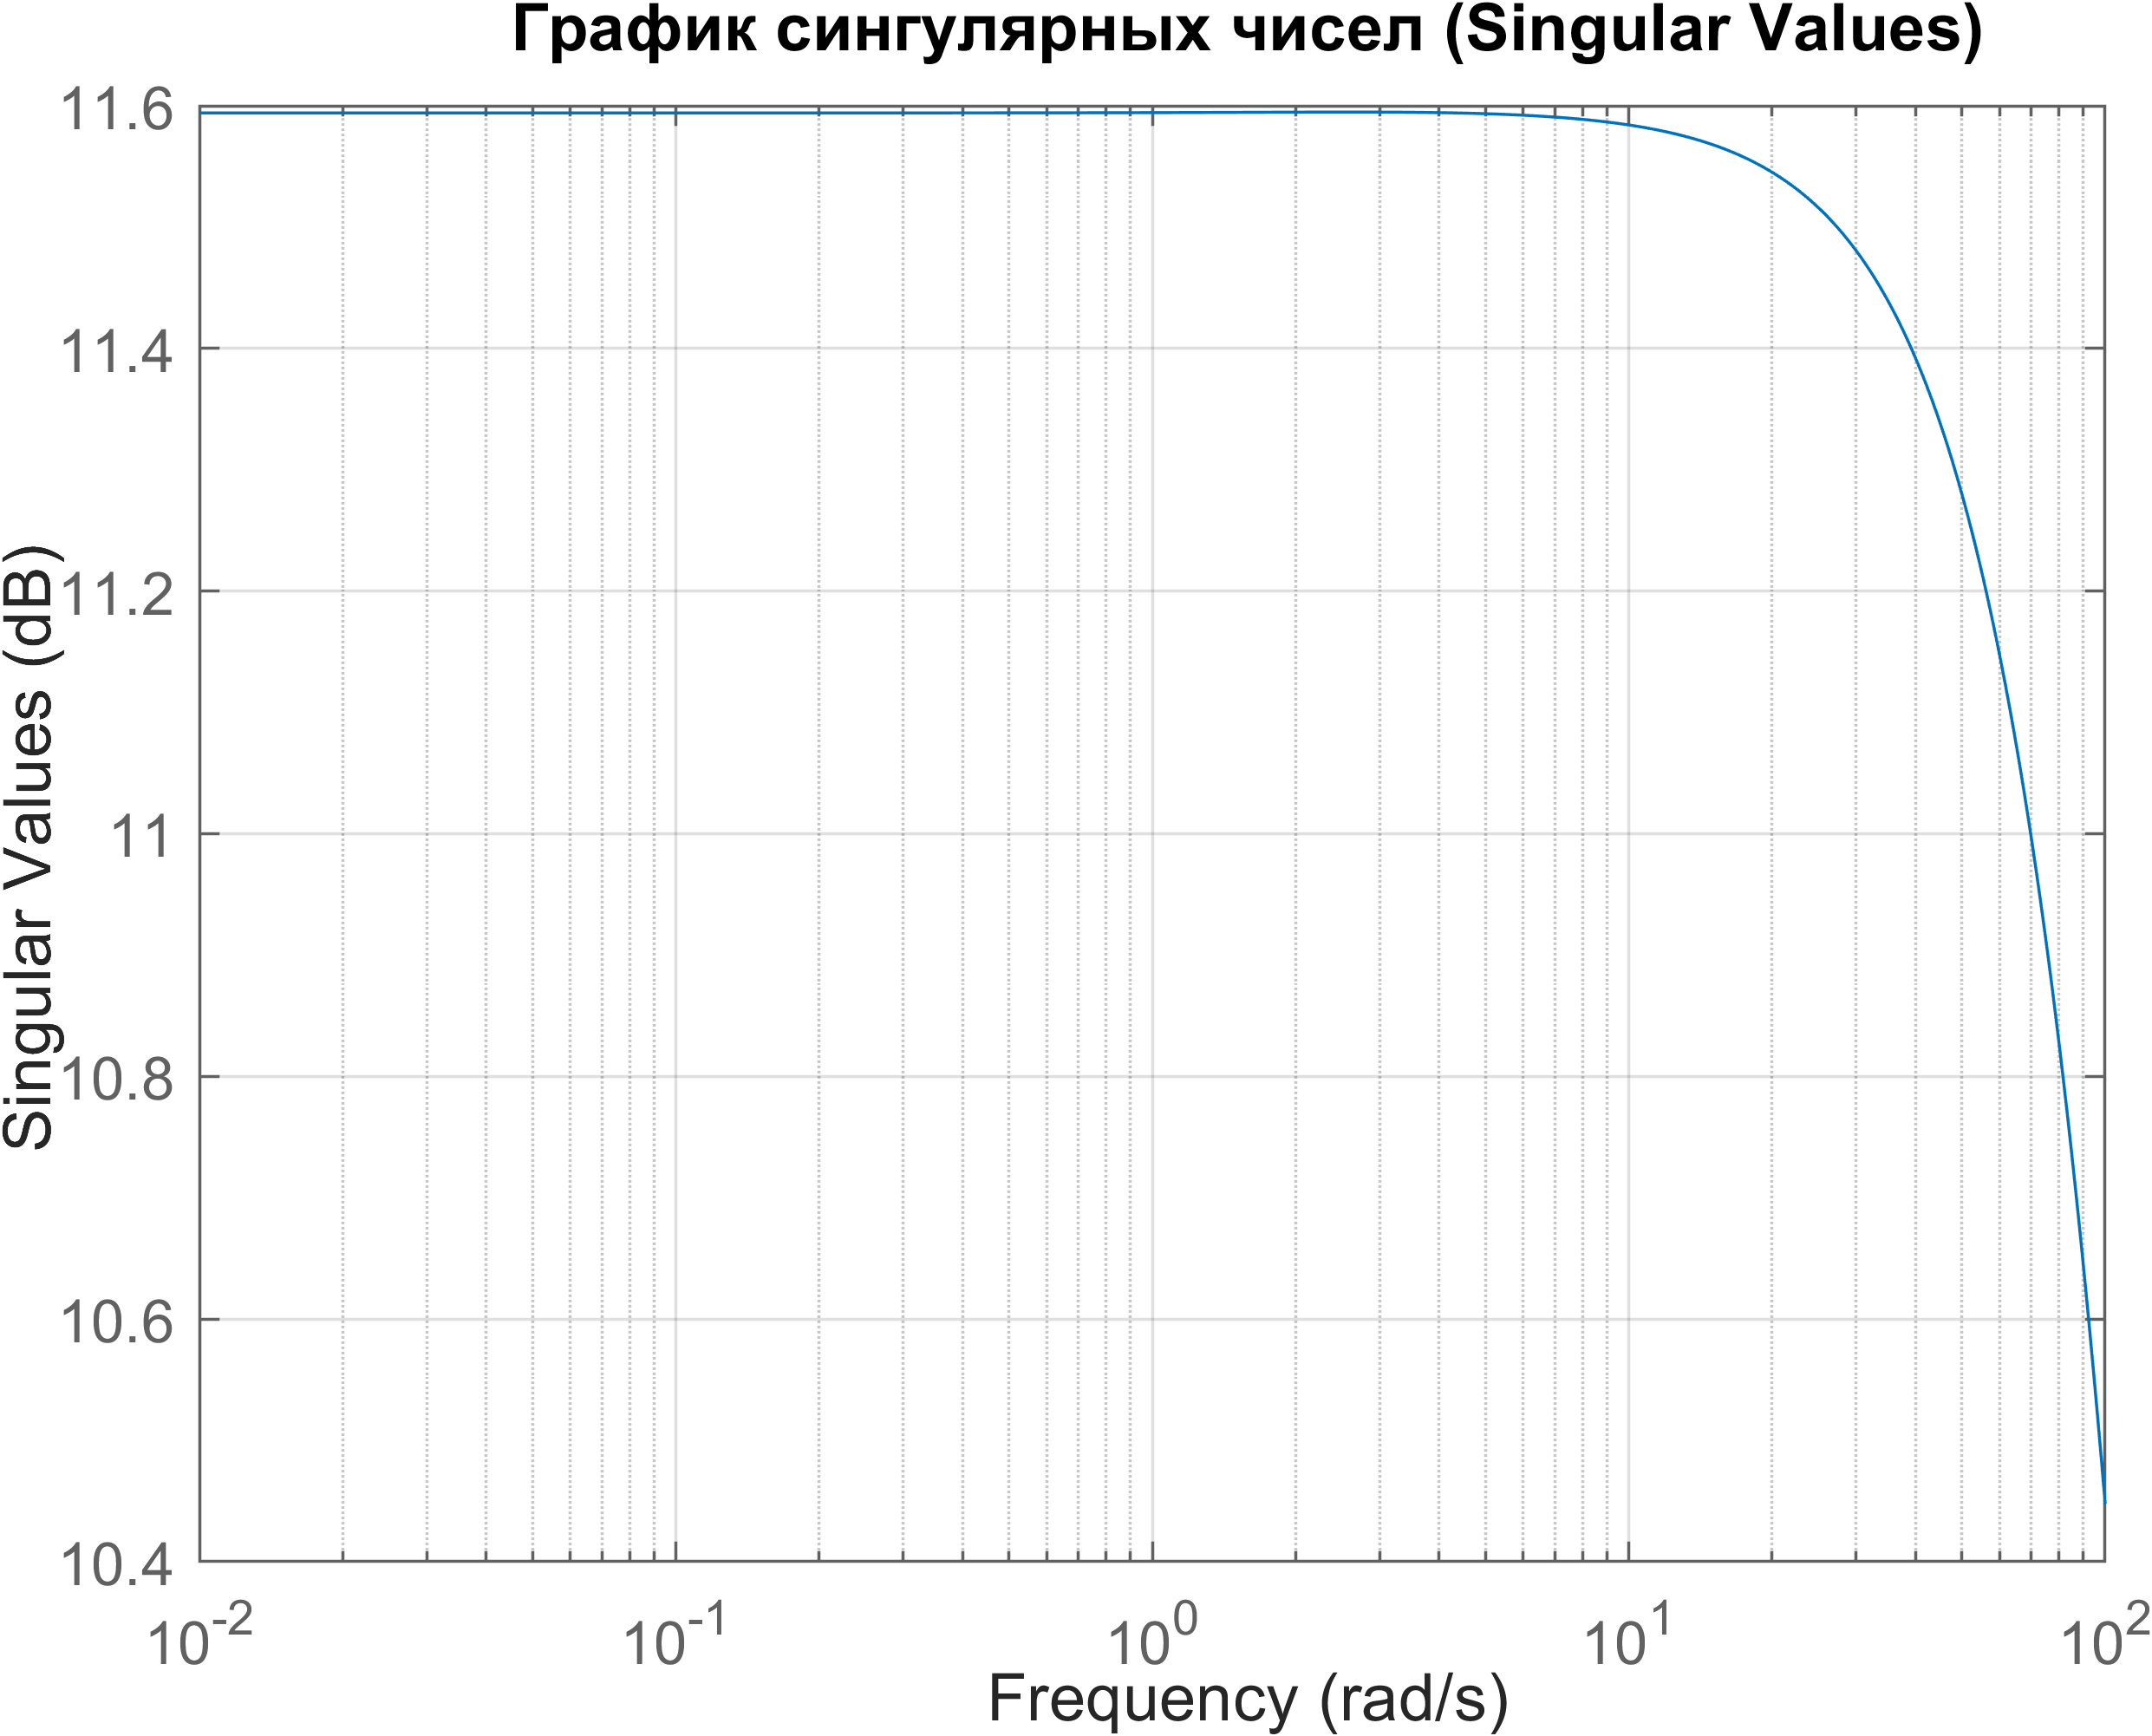
\includegraphics[width=0.8\linewidth]{figs/5_sigma.png}
    \caption{Сингулярные числа $\underset{w\rightarrow z}{W}(s)$}
    \label{fig:5sigma}
\end{figure}
\noindent Найдем нормы $\underset{w\rightarrow z}{W}(s)$:
\begin{equation*}
    ||\underset{w\rightarrow z}{W}(s)||_{H2}=36.2207,\quad
    ||\underset{w\rightarrow z}{W}(s)||_{H\infty}=3.7996.
\end{equation*}
Как видно из графика сингулярных числе, наихудшая частота возмущения $1$.
Таким образом, зададимся двумя возмущениями:
\begin{equation*}
    w_1(t)=\begin{bmatrix}
        sin(t)\\
        0
    \end{bmatrix},\quad
    w_2(t)=\begin{bmatrix}
        sin(100t)\\
        0
    \end{bmatrix}.
\end{equation*}
С помощью SIMULINK (см. \autoref{fig:slx}) для каждого из выбранных вариантов внешнего возмущения $w$ выполним 
компьютерное моделирование замкнутой системы при нулевых начальных условиях
на объекте управления и построим графики компонент регулируемого выхода
$z(t)$, которые можно увидеть на \autoref{fig:5sim}.
\begin{figure}[H]
    \centering
    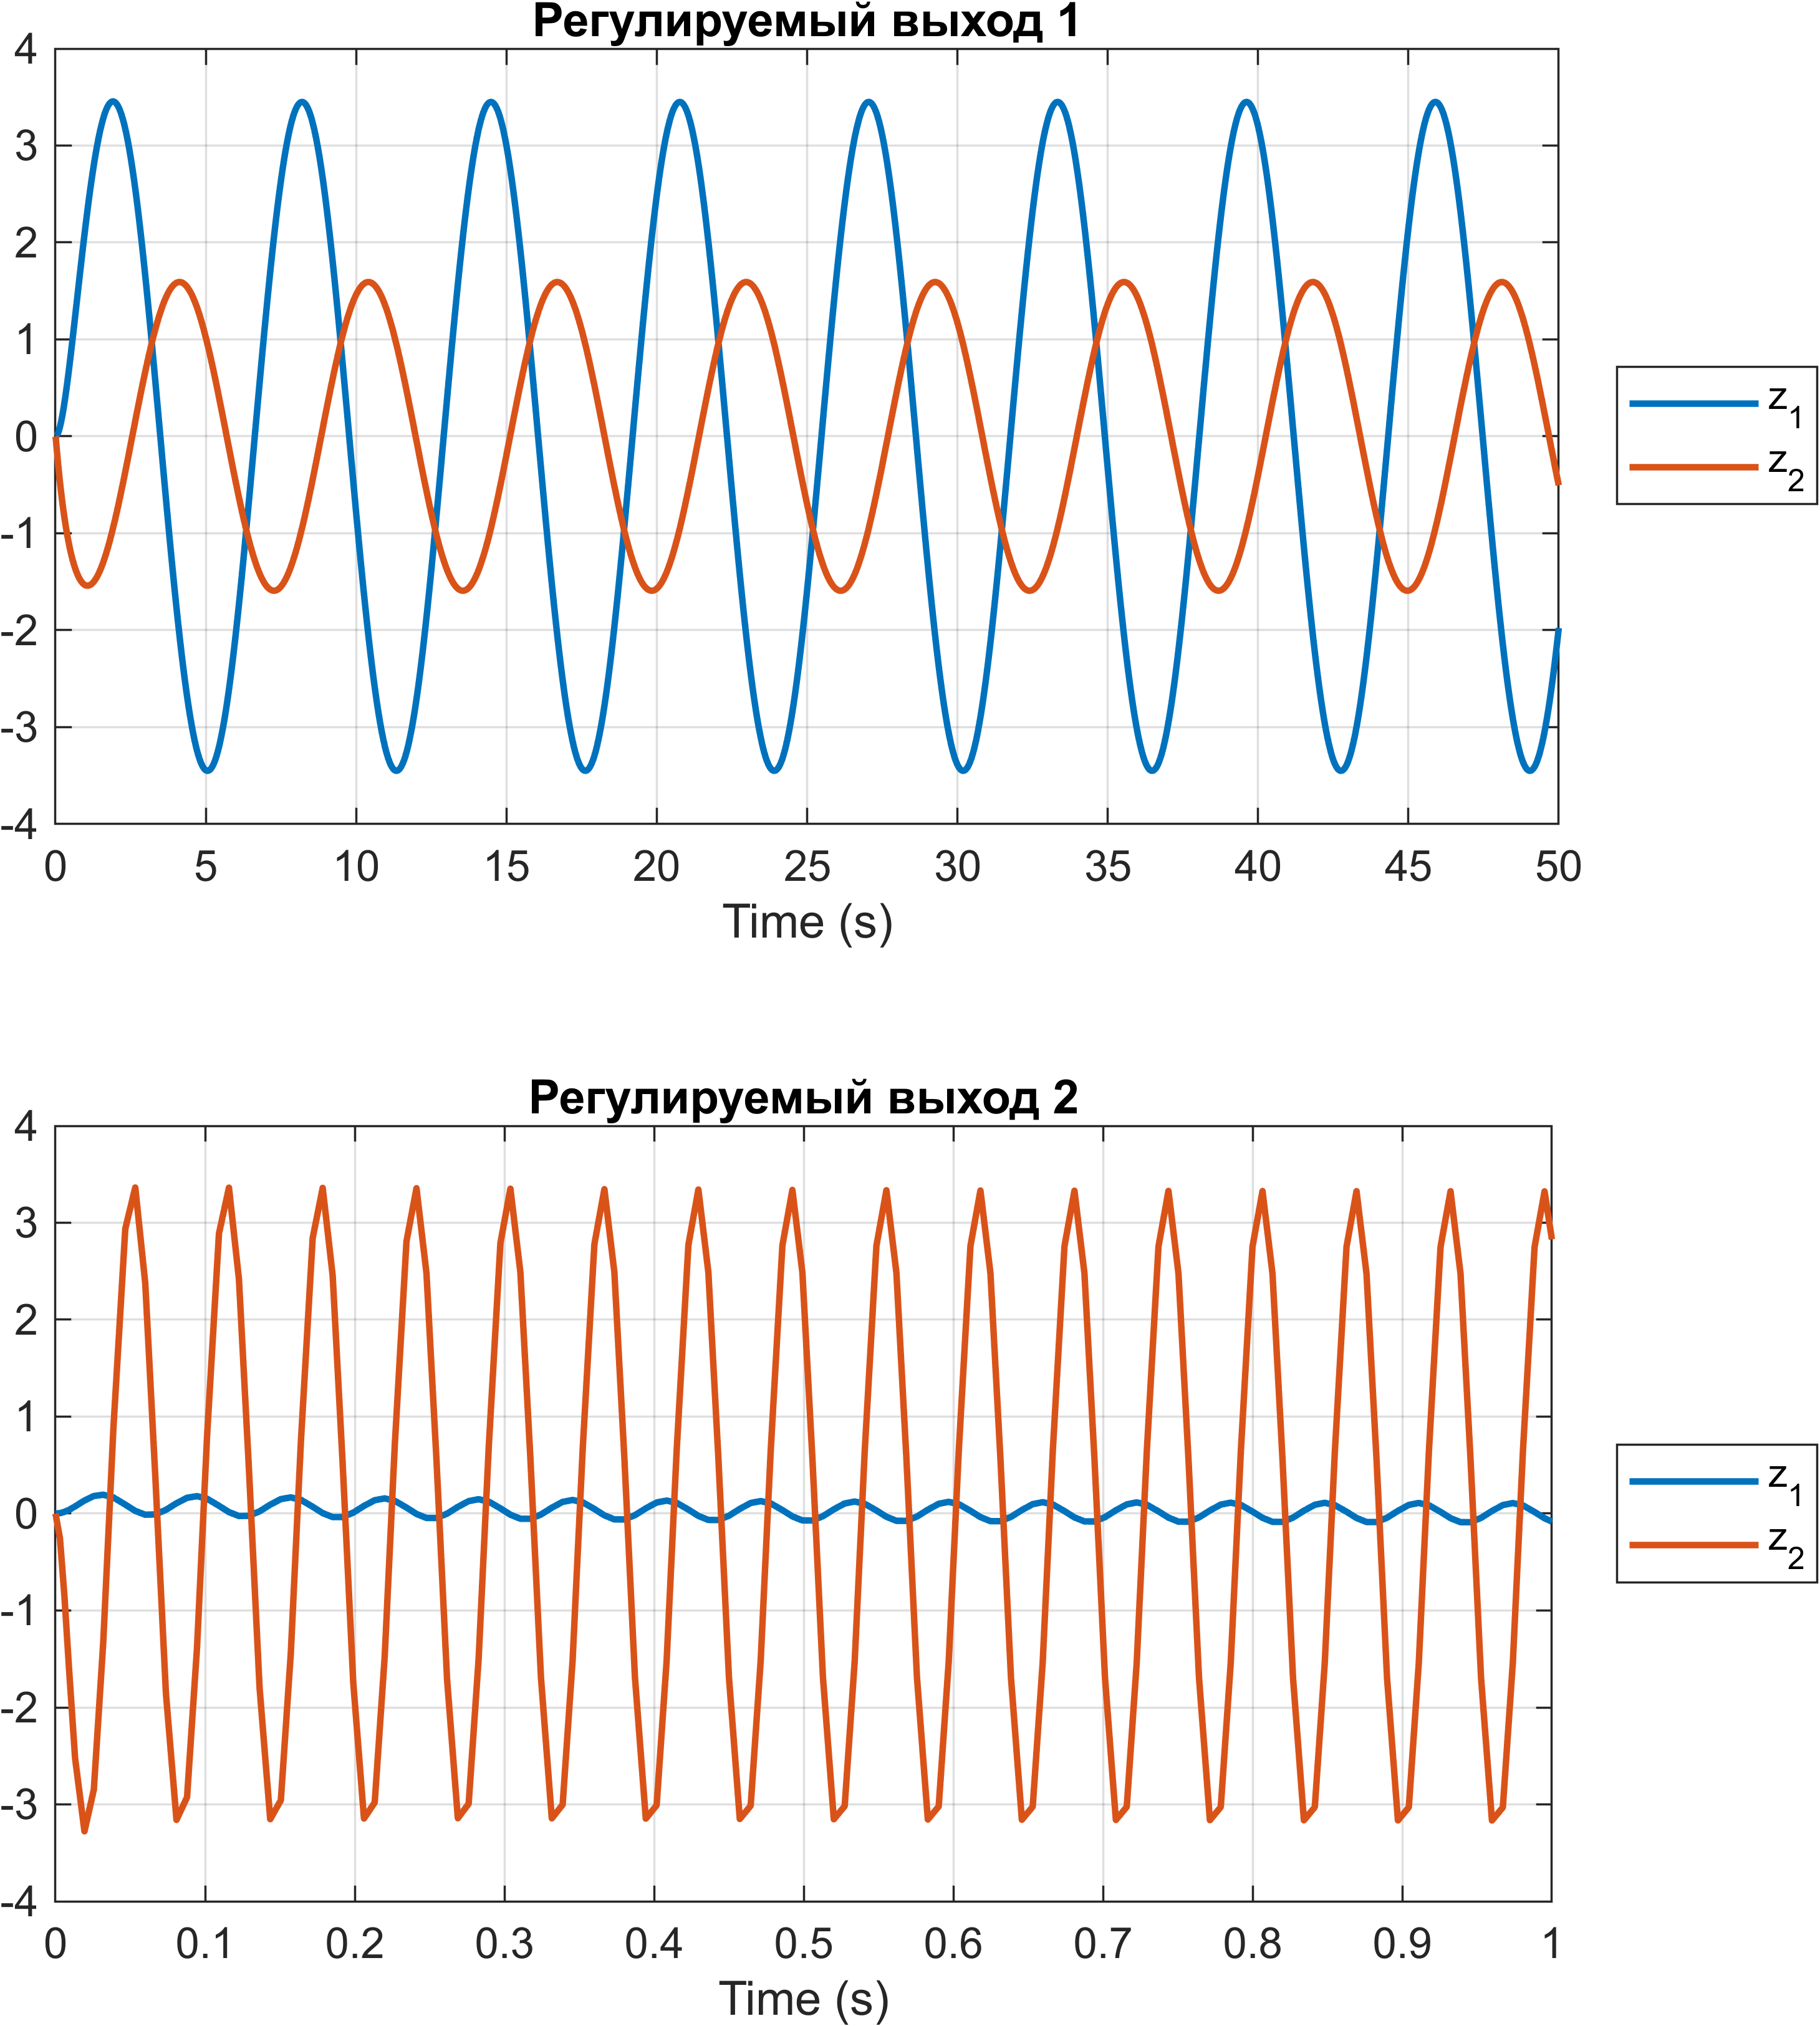
\includegraphics[width=1\linewidth]{figs/5_sim.png}
    \caption{График $z(t)$ при $w_1(t)$ и $w_2(t)$}
    \label{fig:5sim}
\end{figure}

\subsubsection{Выводы}

Из графиков видно, что полностью побороть помеху не удалось, и регулируемый выход 
колеблется около нуля, что естественно, так как нашей задачей было минимизировать норму H infinity. 
Также видно, что на частоте 1 амплитуда колебаний точно такая же как и при частоте 100,
что говорит о том, что регулятор выполняется свою работу, это видно и по АЧХ, которая
выравнялась по сравнению с H2-регулятором \autoref{fig:1sigma}, так же отмечу, что
норма H infinity меньше в два раза чем у H2-регулятора, что, опять же, подтверждает
что регулятор выполняет свою работу, минимизируя норму H infinity.



\subsection{Гамма побольше}

Аналогично синтезируем H infinity регулятор, но уже для значительно большего $\gamma=500$.
Используя \texttt{icare} получим
\begin{equation*}
    K=\begin{bmatrix}
        -10.0006&	-4.4724
    \end{bmatrix}.
\end{equation*}
Передаточная матрица замкнутой системы от внешнего возмущения $w$ к выходу $z$:
\begin{equation*}
    \underset{w\rightarrow z}{W}(s)=\begin{bmatrix}
        \dfrac{10 s + 54.72}{s^2 + 4.472 s + 10} & 0 \\[2ex]
        \dfrac{ -14.47 s - 10}{s^2 + 4.472 s + 10} & 0
    \end{bmatrix}
\end{equation*}
График покомпонентных АЧХ $\underset{w\rightarrow z}{W}(s)$ представлен на \autoref{fig:6bodemag}.
\begin{figure}[H]
    \centering
    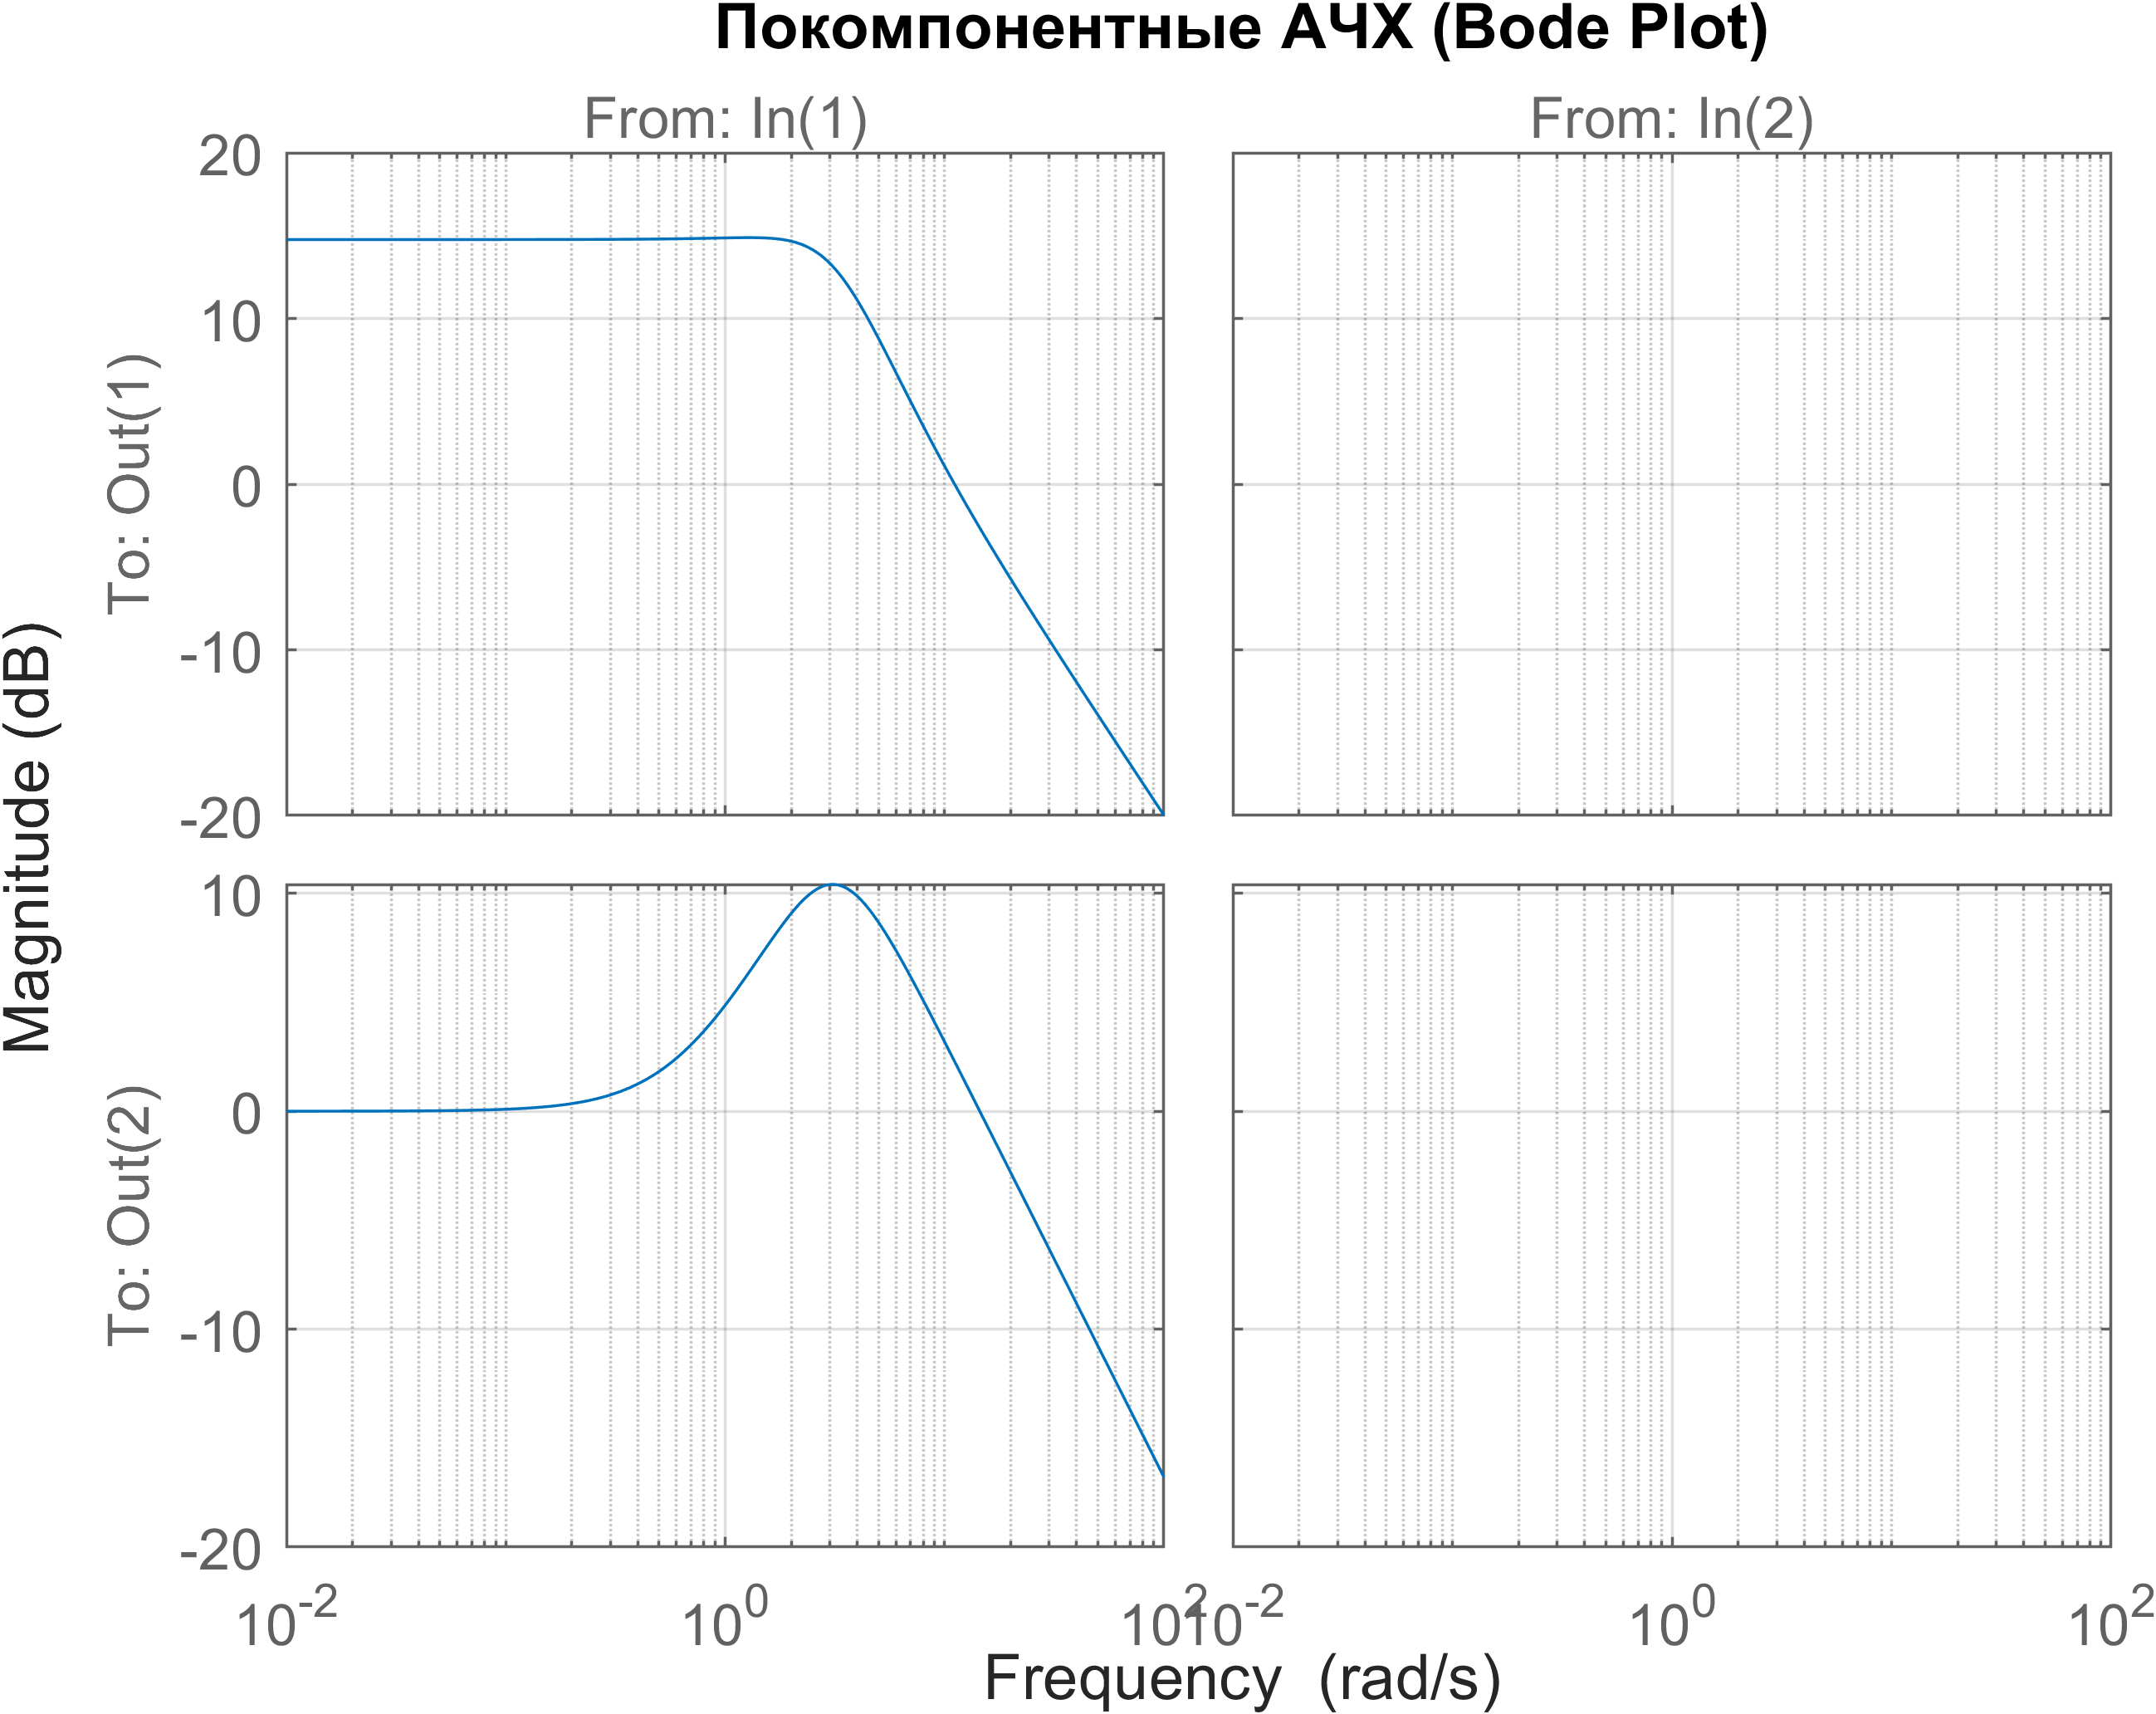
\includegraphics[width=0.8\linewidth]{figs/6_bodemag.png}
    \caption{Покомпонентные АЧХ $\underset{w\rightarrow z}{W}(s)$}
    \label{fig:6bodemag}
\end{figure}
График сингулярных чисел $\underset{w\rightarrow z}{W}(s)$ представлен на \autoref{fig:6sigma}.
\begin{figure}[H]
    \centering
    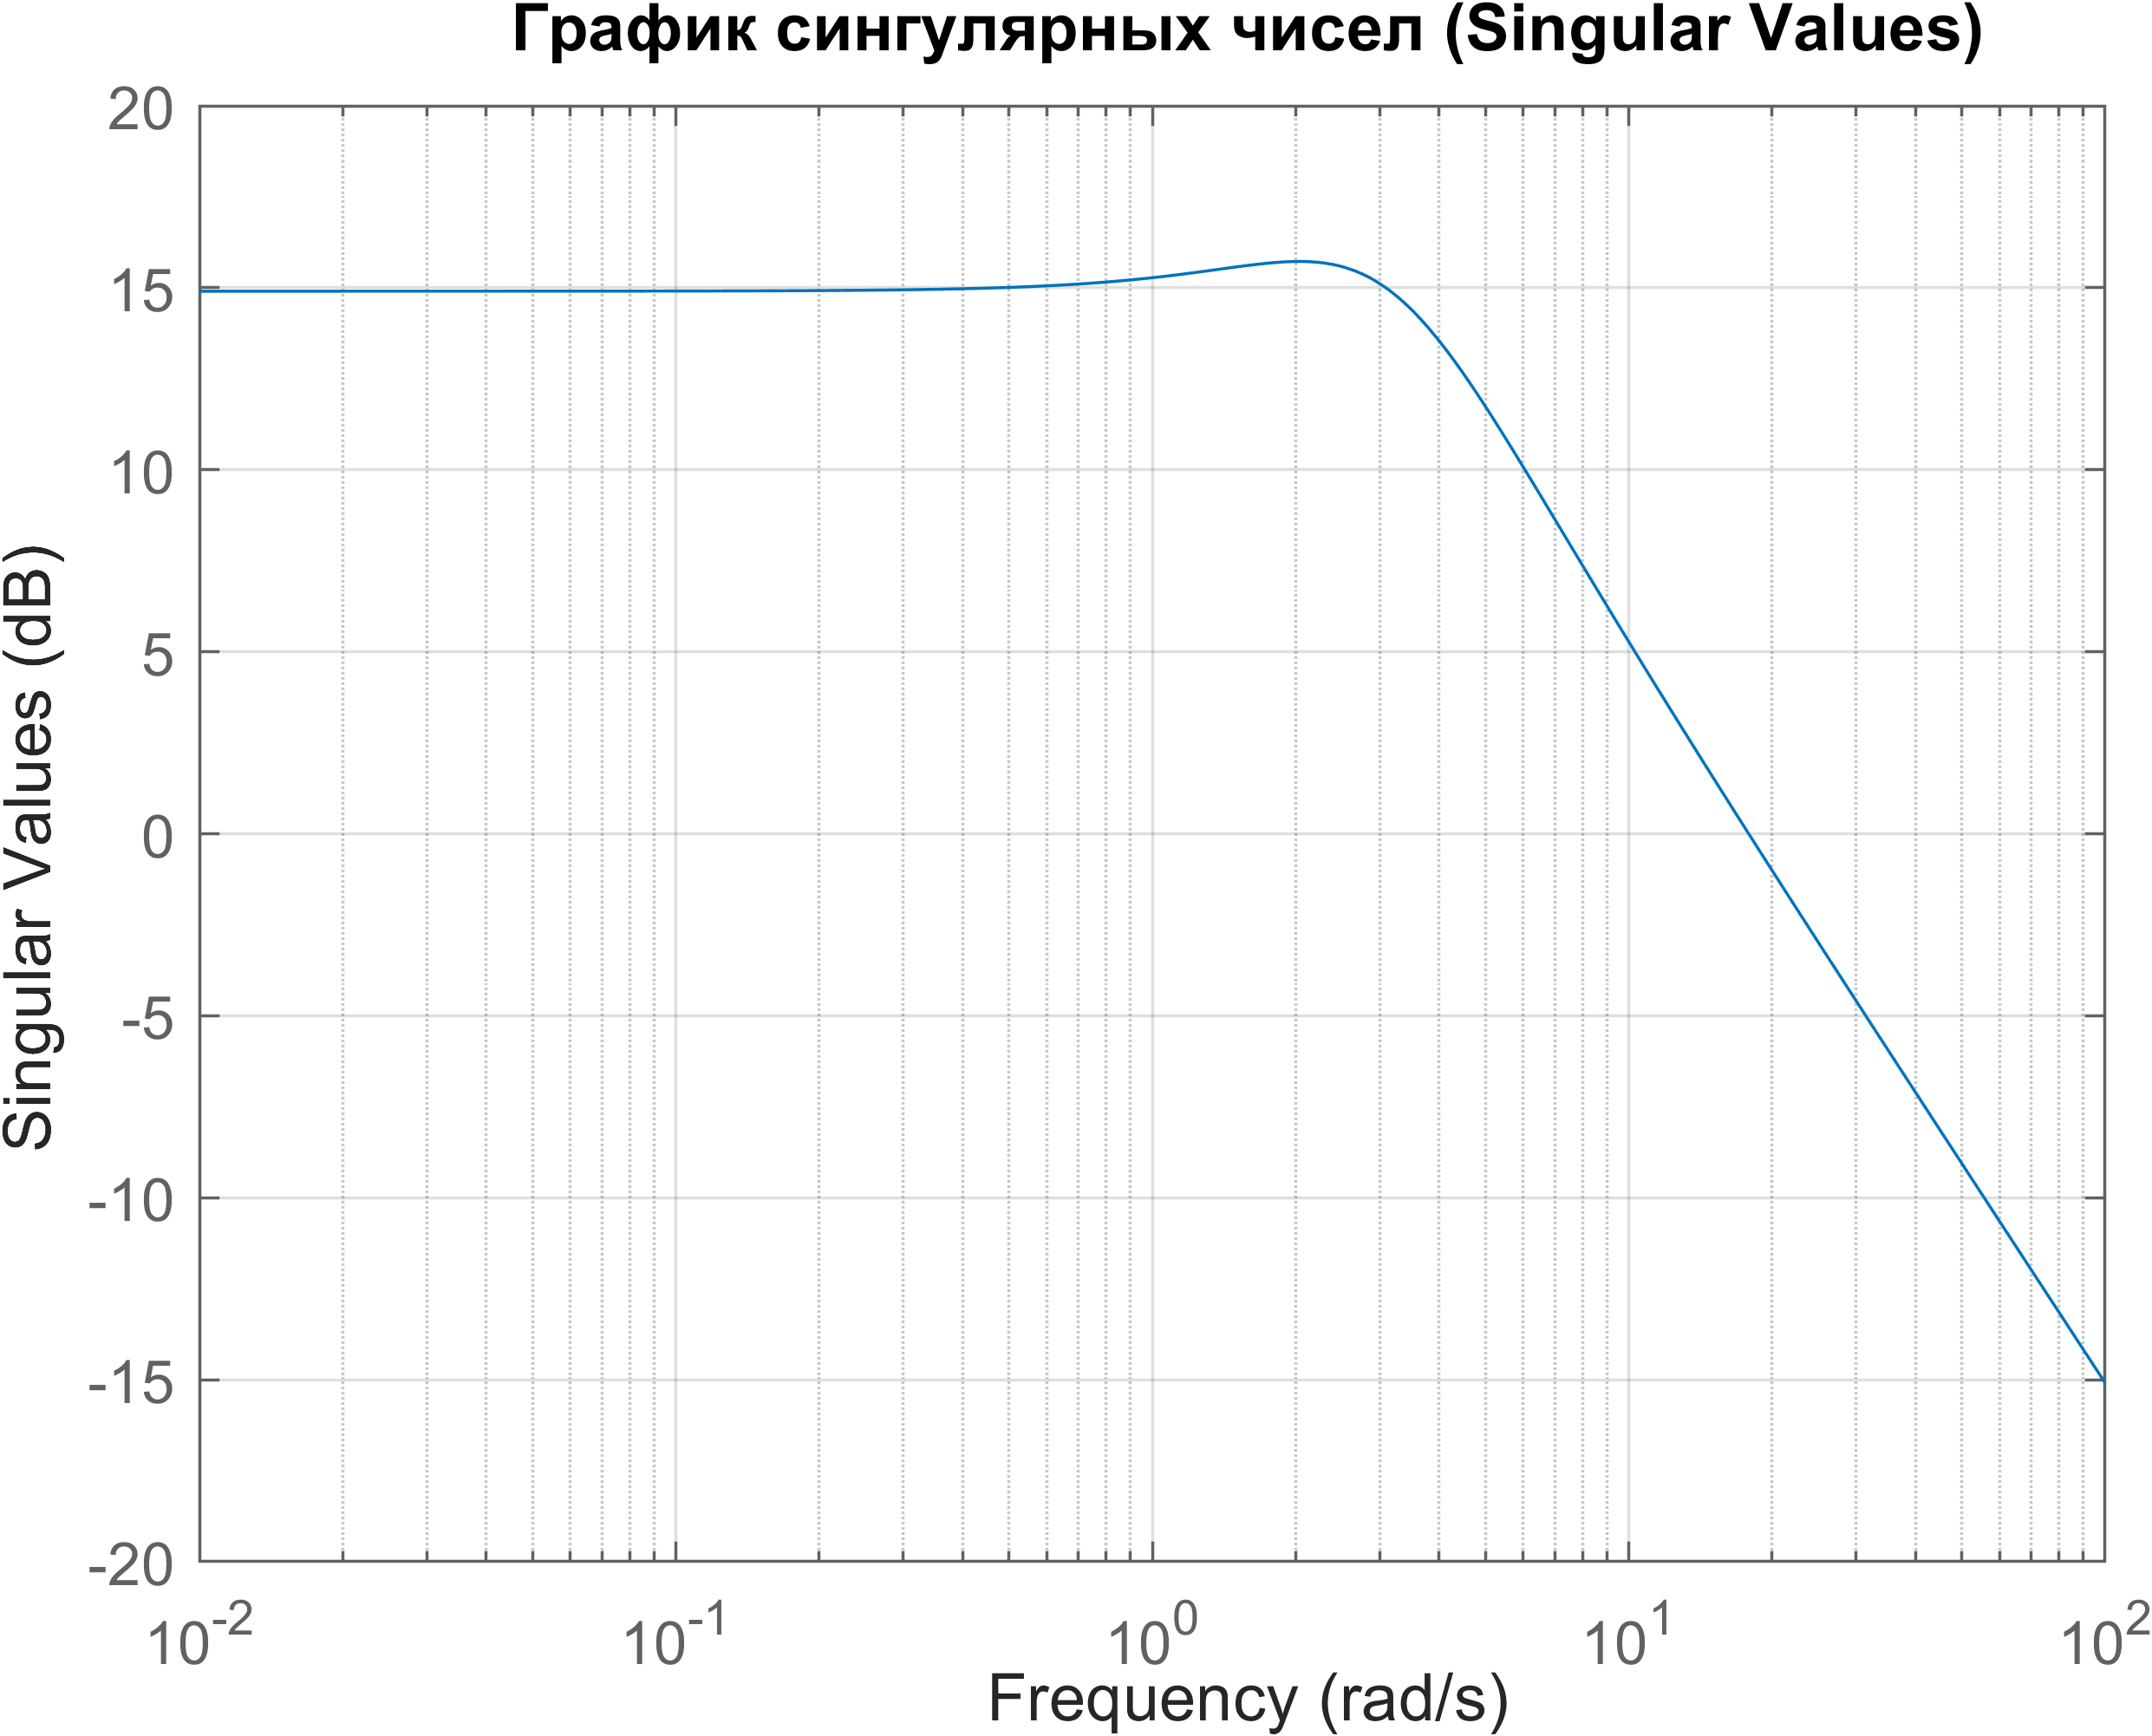
\includegraphics[width=0.8\linewidth]{figs/6_sigma.png}
    \caption{Сингулярные числа $\underset{w\rightarrow z}{W}(s)$}
    \label{fig:6sigma}
\end{figure}
\noindent Найдем нормы $\underset{w\rightarrow z}{W}(s)$:
\begin{equation*}
    ||\underset{w\rightarrow z}{W}(s)||_{H2}=8.3183,\quad
    ||\underset{w\rightarrow z}{W}(s)||_{H\infty}=6.1115.
\end{equation*}
Как видно из графика сингулярных числе, наихудшая частота возмущения $2$.
Таким образом, зададимся двумя возмущениями:
\begin{equation*}
    w_1(t)=\begin{bmatrix}
        sin(2t)\\
        0
    \end{bmatrix},\quad
    w_2(t)=\begin{bmatrix}
        sin(20t)\\
        0
    \end{bmatrix}.
\end{equation*}
С помощью SIMULINK (см. \autoref{fig:slx}) для каждого из выбранных вариантов внешнего возмущения $w$ выполним 
компьютерное моделирование замкнутой системы при нулевых начальных условиях
на объекте управления и построим графики компонент регулируемого выхода
$z(t)$, которые можно увидеть на \autoref{fig:6sim}.
\begin{figure}[H]
    \centering
    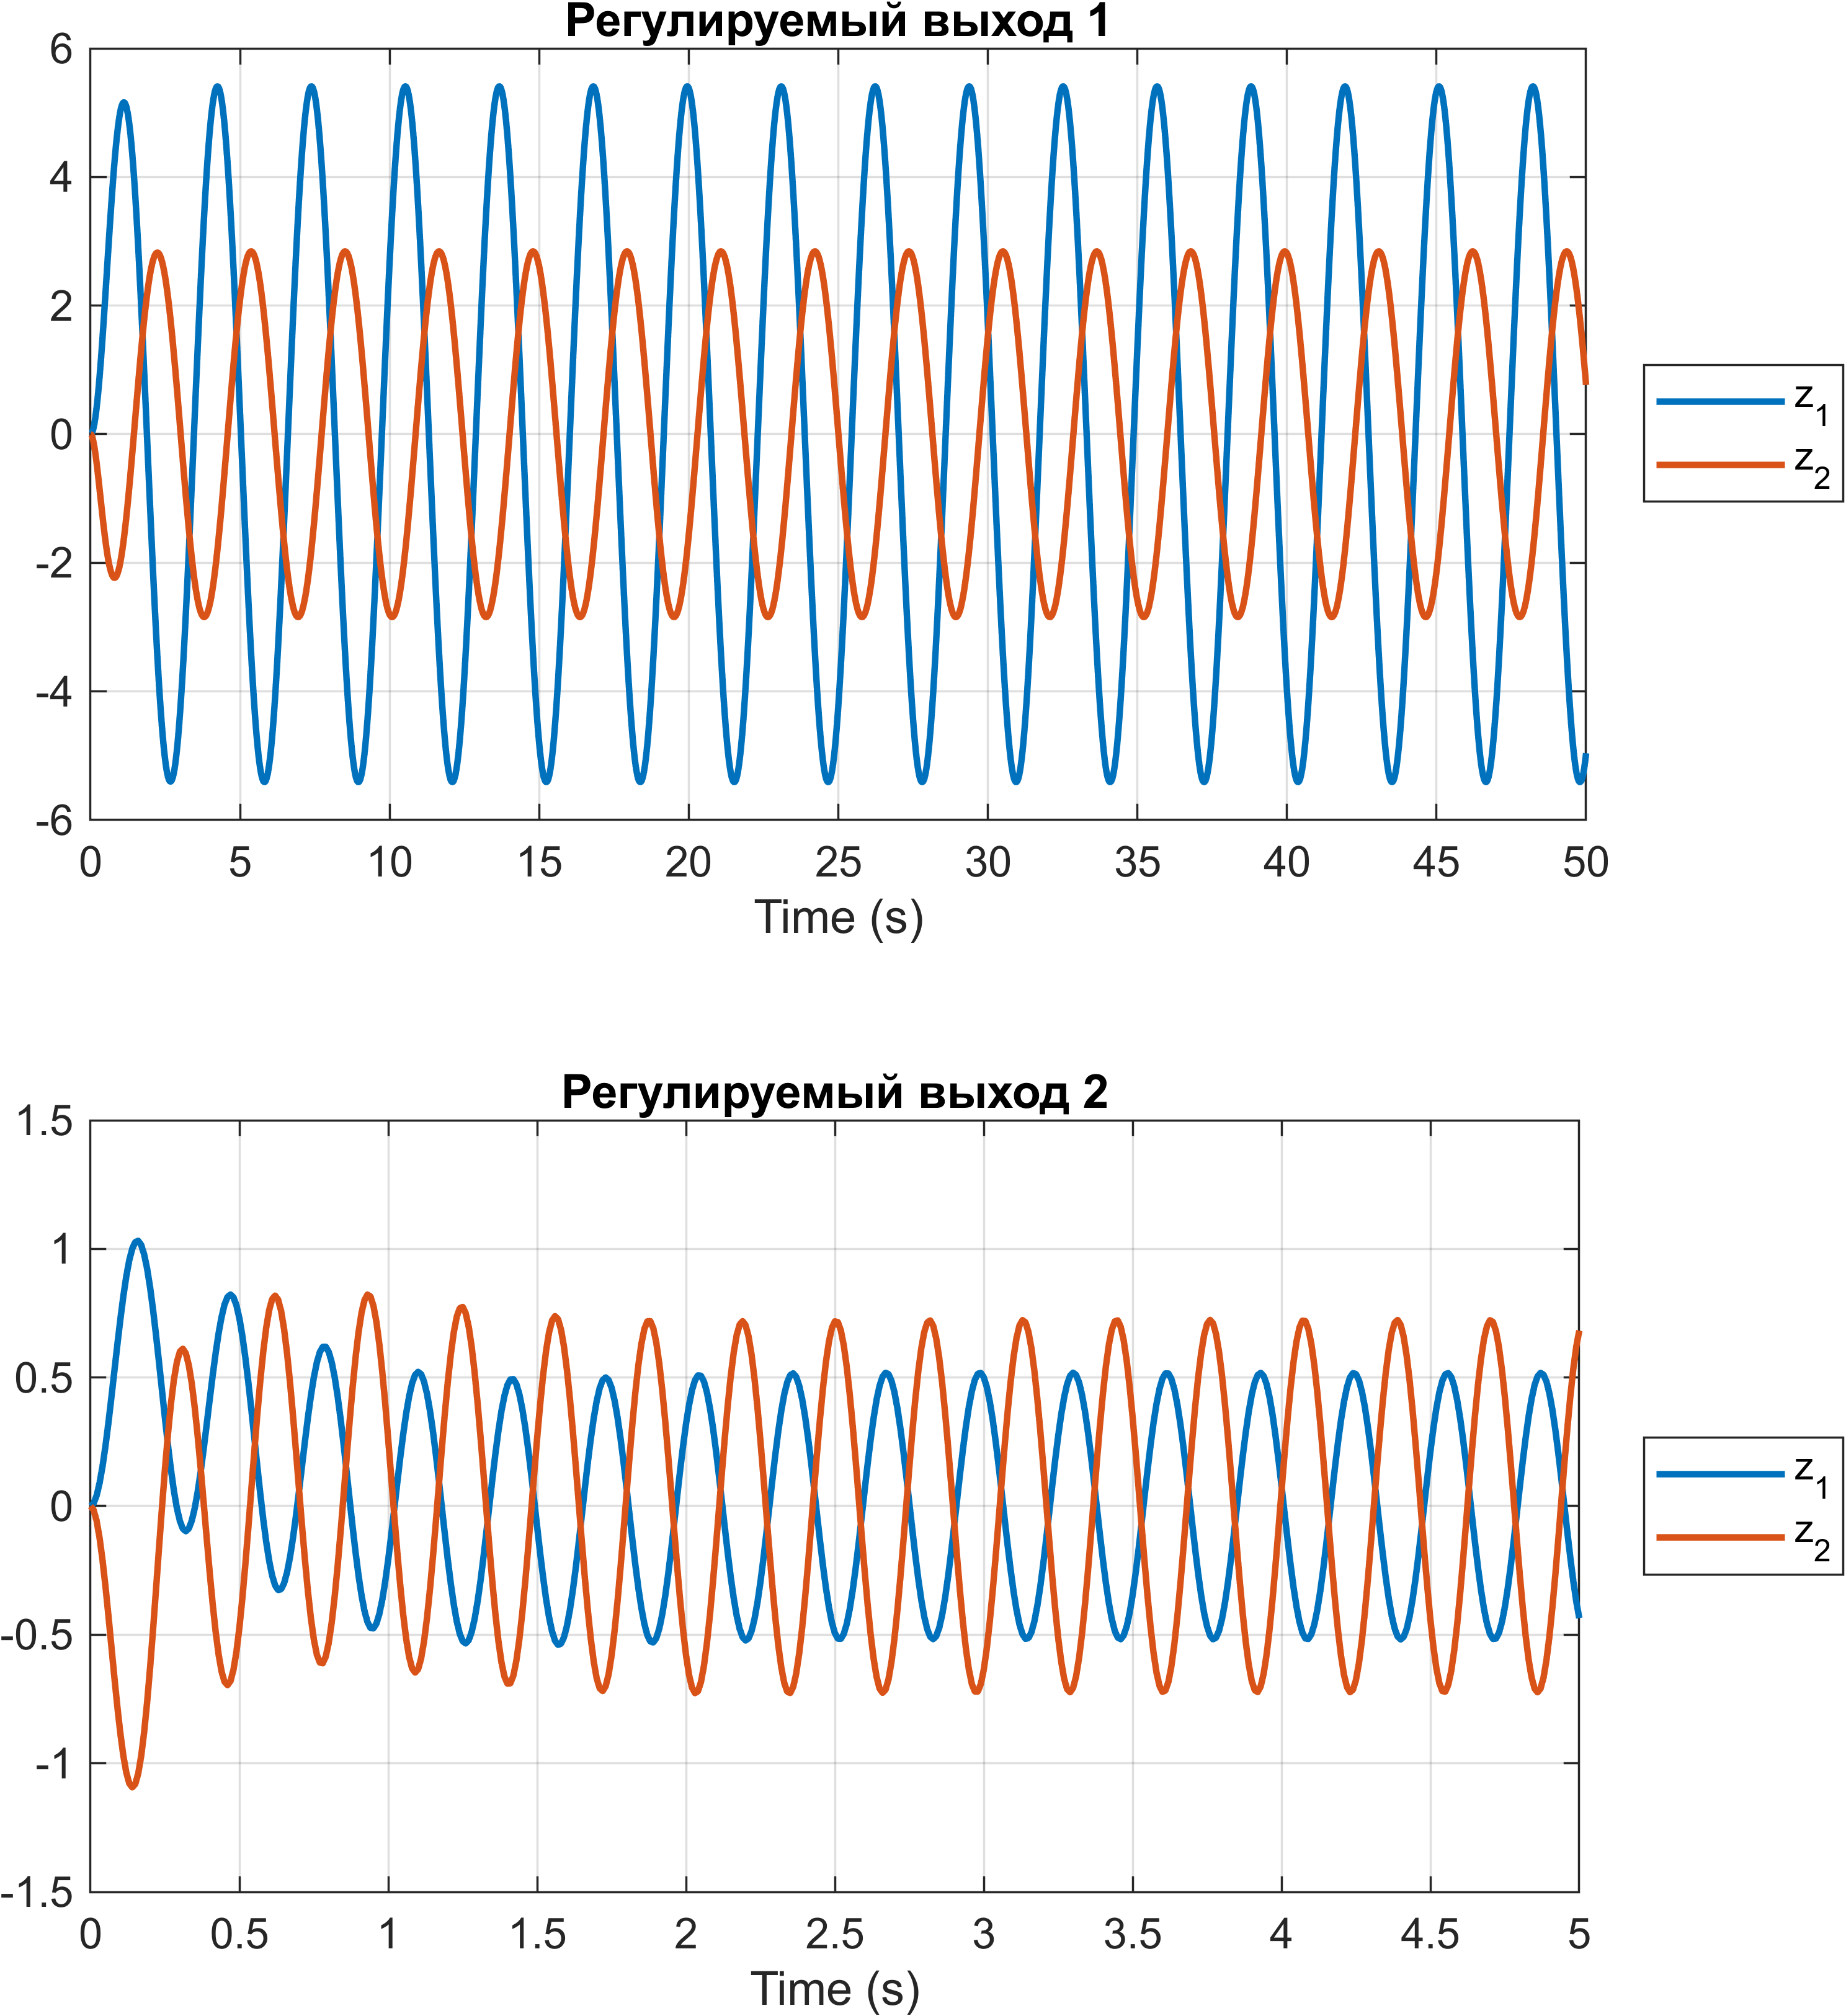
\includegraphics[width=1\linewidth]{figs/6_sim.png}
    \caption{График $z(t)$ при $w_1(t)$ и $w_2(t)$}
    \label{fig:6sim}
\end{figure}

\subsubsection{Выводы}

Из графиков видно, что полностью побороть помеху не удалось, и регулируемый выход 
колеблется около нуля, что естественно, так как нашей задачей было минимизировать норму H infinity. 
Но также видно, что на частоте 2 амплитуда колебаний в несколько раз больше чем при частоте 20,
что говорит о том, что регулятор плохо выполняется свою работу по минимизации нормы H infinity, это видно и по АЧХ, которая
повторяет за H2-регулятором \autoref{fig:1sigma}, так же отмечу, что
нормы H infinity повторяют таковые у H2-регулятора. Из этого можно сделать вывод, что
при большой гамме H infinity регулятор становится H2-регулятором.





\section{Синтез H infinity регулятора по выходу}

Будем использовать ($C_{Z1},\ D_{Z1}$) матрицы для регулируемого выхода, и обозначать
без цифр ($C_{Z},\ D_{Z}$). 

\subsection{Минимальная гамма}

Синтезируем H infinity регулятор вида $u=Kx$ по состоянию путем решения матричного
уравнения Риккати:
\begin{equation}
    \label{eq:ric4}
    \begin{cases}
        AP+PA^T+B_wB_w^T-PC^T(D_wD_w^T)^{-1}CP+\gamma^{-2}PC_Z^TC_ZP=0,\\
        L=-P(I-\gamma^{-1}QP)^{-1}(C+\gamma^{-2}D_wB_w^TQ)^T(D_wD_w^T)^{-1}.
    \end{cases}
\end{equation}
Сначала найдем $K$ через решение уравнения \eqref{eq:ric3}, используя \texttt{icare} получим
\begin{equation*}
    K=\begin{bmatrix}
        -10.8240	&-4.7845
    \end{bmatrix}.
\end{equation*}
Найдем $L$ через решение уравнения \eqref{eq:ric4}, используя \texttt{icare} получим
\begin{equation*}
    L=\begin{bmatrix}
        -19.2256&
-10.0980
    \end{bmatrix}^T.
\end{equation*}
Данные матрицы были получены при минимальном $\gamma=14$.
Передаточная матрица замкнутой системы от внешнего возмущения $w$ к выходу $z$:
\begin{equation*}
    \underset{w\rightarrow z}{W}(s)=\begin{bmatrix}
        \underset{w\rightarrow z}{W_1}(s) & \underset{w\rightarrow z}{W_2}(s)\\
        \underset{w\rightarrow z}{W_3}(s) & \underset{w\rightarrow z}{W_4}(s)
    \end{bmatrix},
\end{equation*}
где
\begin{gather*}
    \underset{w\rightarrow z}{W_1}(s)=\dfrac{ 10 s^3 + 250.1 s^2 + 1369 s + 1129}{s^4 + 24.01 s^3 + 112.9 s^2 + 256.4 s + 109.3}\\
    \underset{w\rightarrow z}{W_2}(s)=\dfrac{-2564 s - 1093}{s^4 + 24.01 s^3 + 112.9 s^2 + 256.4 s + 109.3}\\
    \underset{w\rightarrow z}{W_3}(s)=\dfrac{-256.4 s^2 - 365.7 s - 109.3}{s^4 + 24.01 s^3 + 112.9 s^2 + 256.4 s + 109.3}\\
    \underset{w\rightarrow z}{W_4}(s)=\dfrac{-256.4 s^3 - 109.3 s^2 - 9.679e-14 s - 4.126e-14}{s^4 + 24.01 s^3 + 112.9 s^2 + 256.4 s + 109.3}
\end{gather*}
График покомпонентных АЧХ $\underset{w\rightarrow z}{W}(s)$ представлен на \autoref{fig:7bodemag}.
\begin{figure}[H]
    \centering
    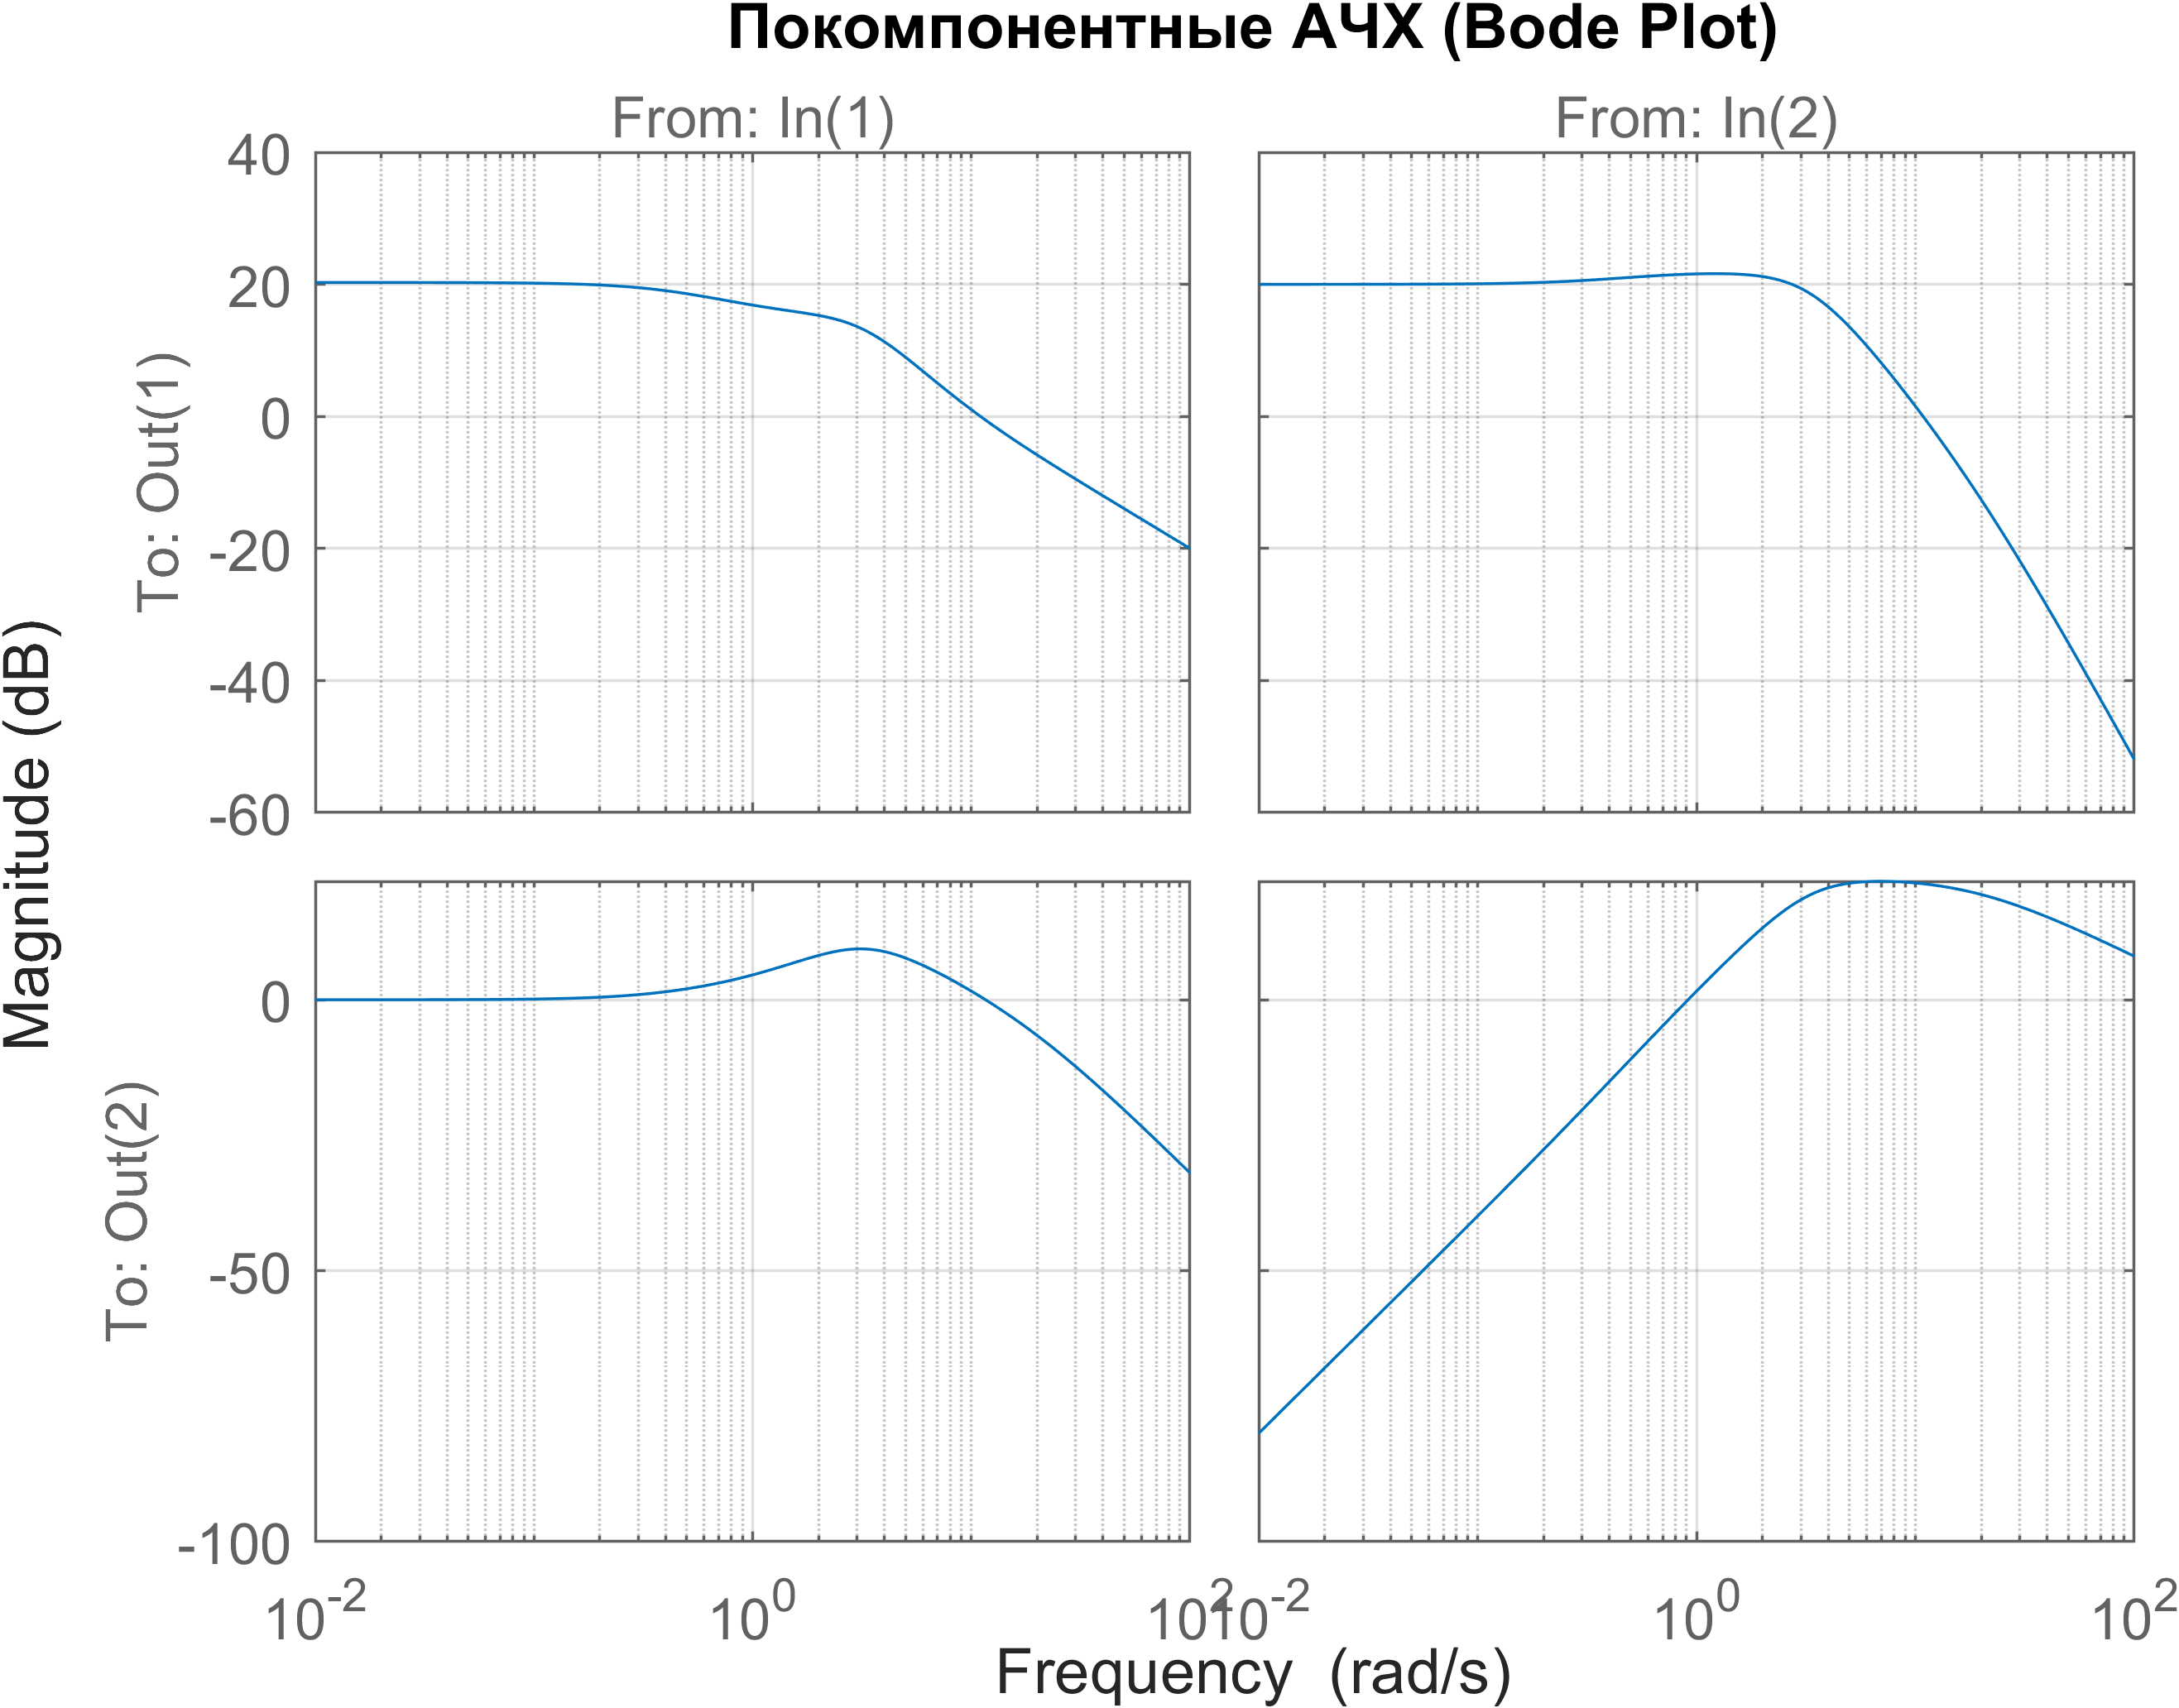
\includegraphics[width=0.8\linewidth]{figs/7_bodemag.png}
    \caption{Покомпонентные АЧХ $\underset{w\rightarrow z}{W}(s)$}
    \label{fig:7bodemag}
\end{figure}
График сингулярных чисел $\underset{w\rightarrow z}{W}(s)$ представлен на \autoref{fig:7sigma}.
\begin{figure}[H]
    \centering
    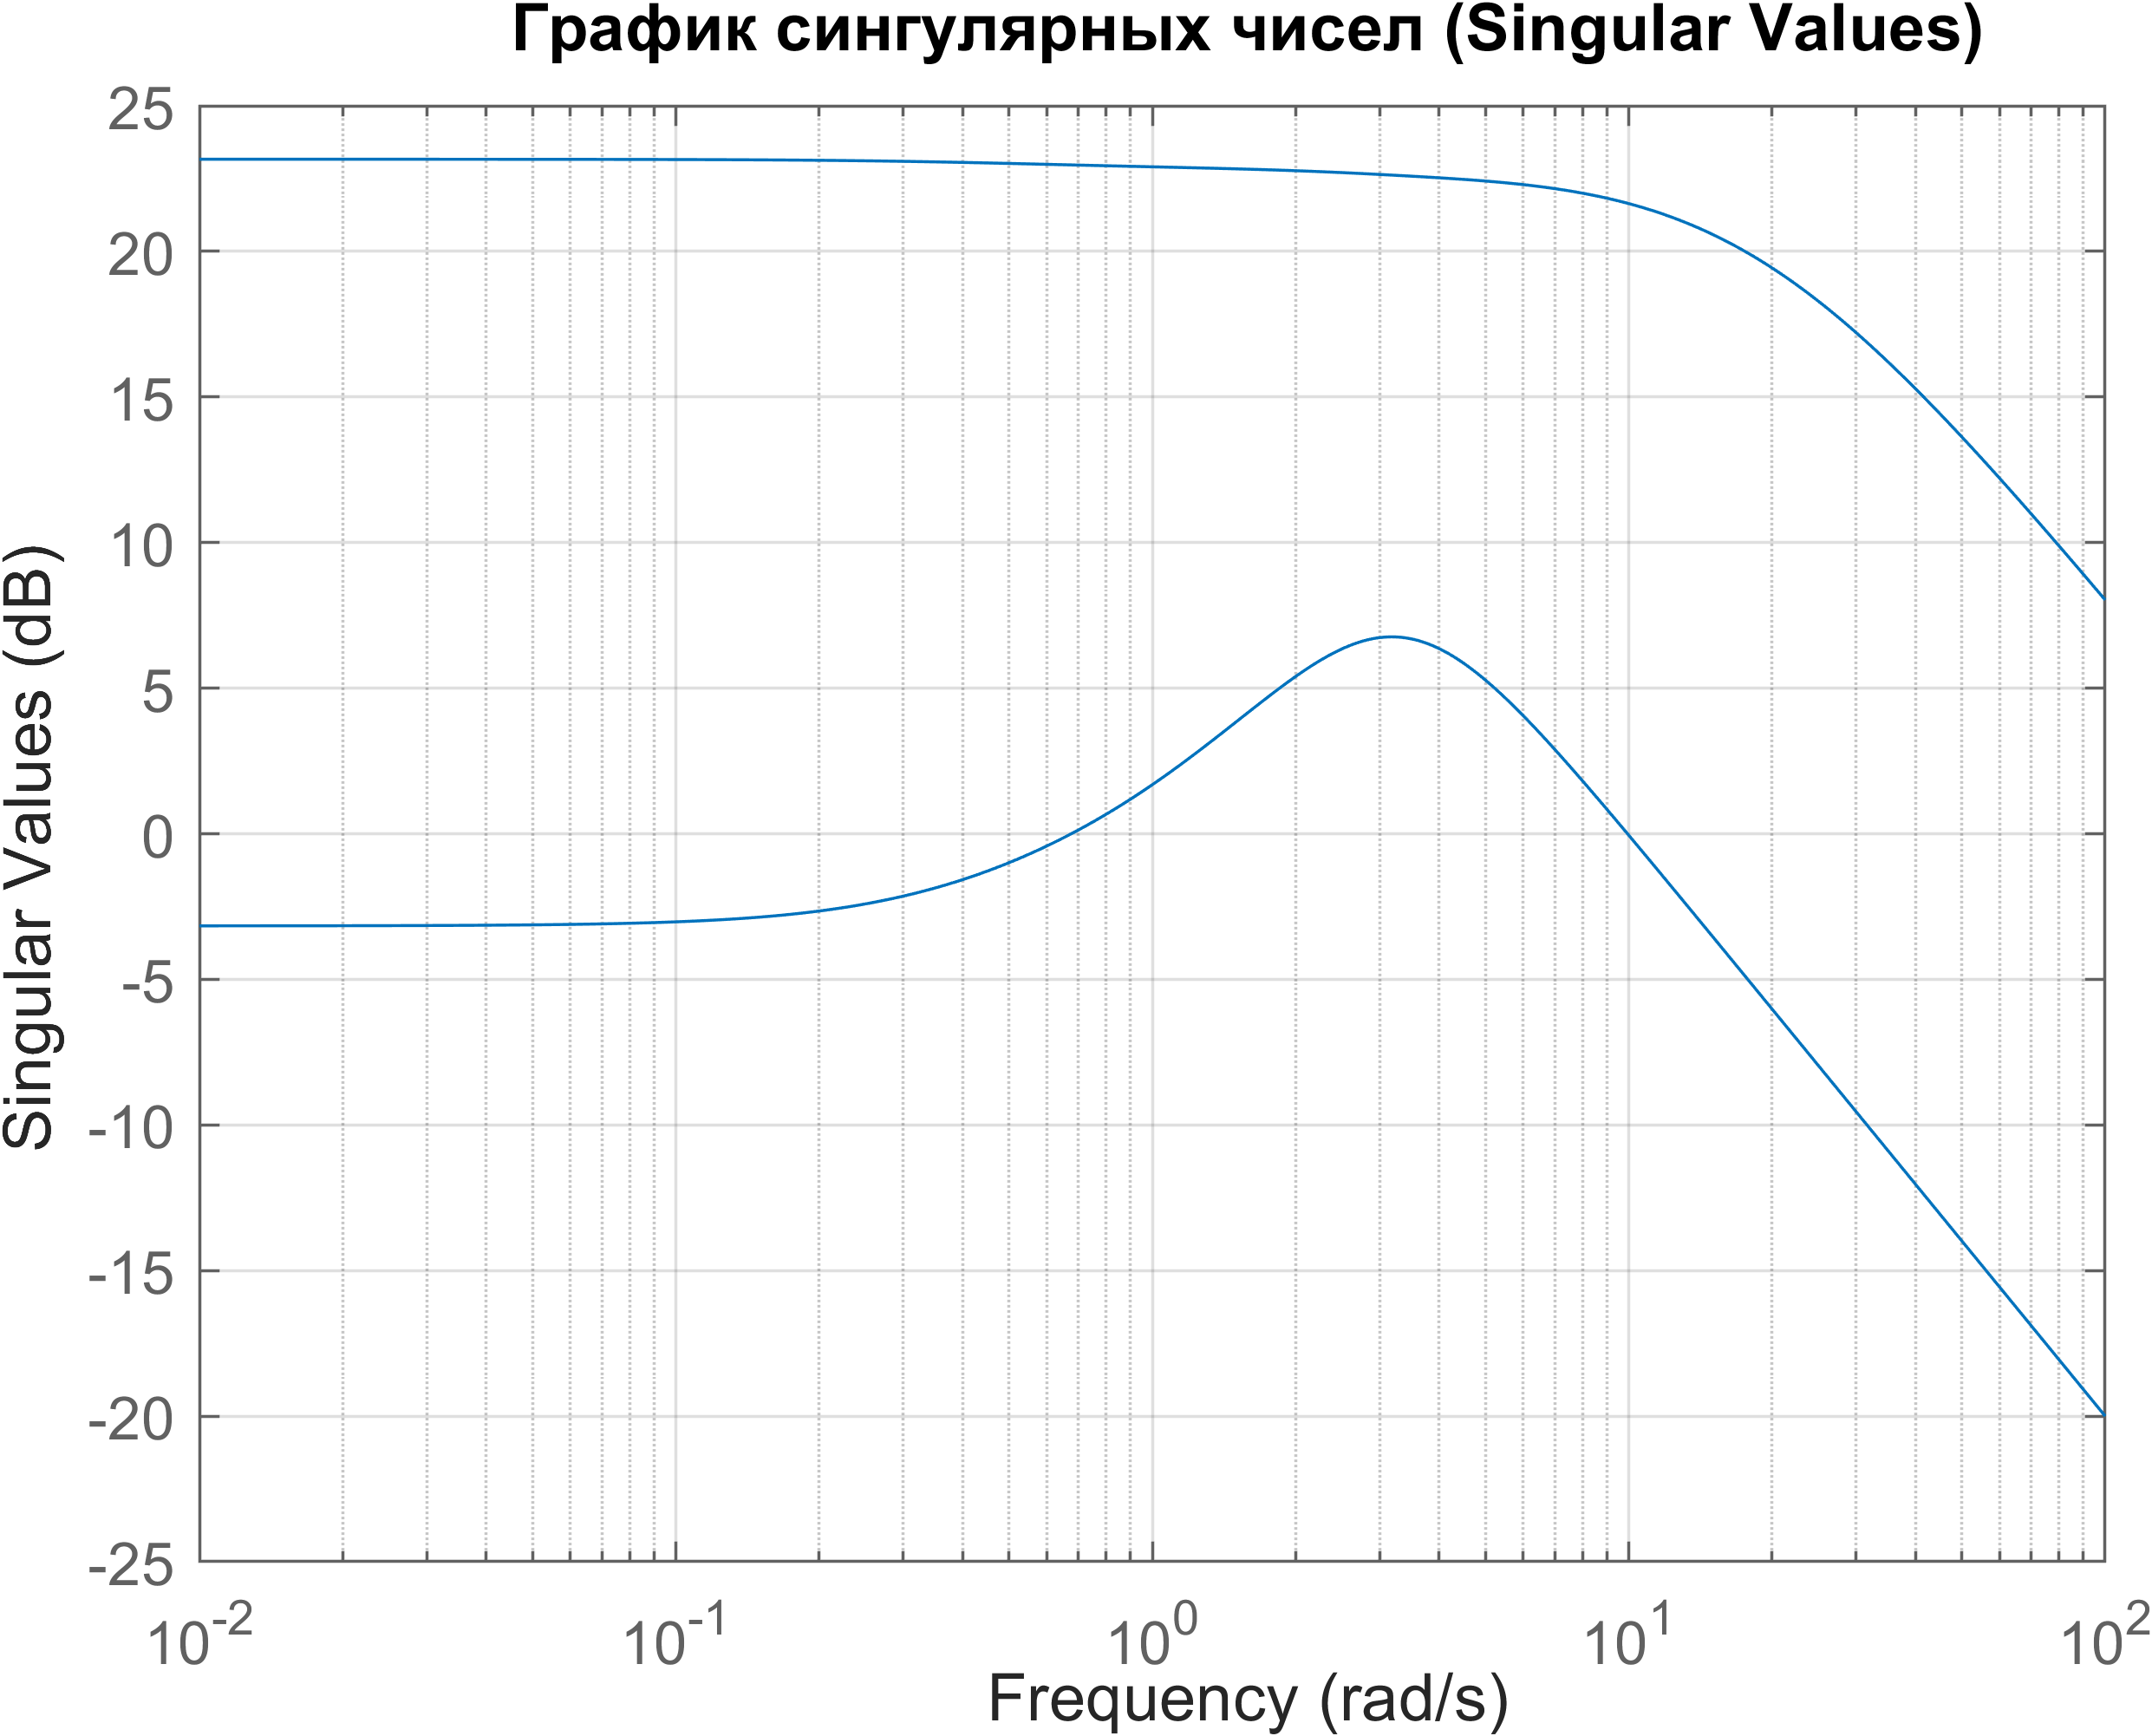
\includegraphics[width=0.8\linewidth]{figs/7_sigma.png} 
    \caption{Сингулярные числа $\underset{w\rightarrow z}{W}(s)$}
    \label{fig:7sigma}
\end{figure}
\noindent Найдем нормы $\underset{w\rightarrow z}{W}(s)$:
\begin{equation*}
    ||\underset{w\rightarrow z}{W}(s)||_{H2}=42.1182,\quad
    ||\underset{w\rightarrow z}{W}(s)||_{H\infty}=14.3952.
\end{equation*}
Как видно из графика сингулярных числе, наихудшая частота возмущения $0.01$.
Таким образом, зададимся двумя возмущениями:
\begin{equation*}
    w_1(t)=\begin{bmatrix}
        sin(0.01t)\\
        0
    \end{bmatrix},\quad
    w_2(t)=\begin{bmatrix}
        sin(100t)\\
        0
    \end{bmatrix}.
\end{equation*}
С помощью SIMULINK (см. \autoref{fig:3slx}) для каждого из выбранных вариантов внешнего возмущения $w$ выполним 
компьютерное моделирование замкнутой системы при нулевых начальных условиях
на объекте управления и построим графики компонент регулируемого выхода
$z(t)$, которые можно увидеть на \autoref{fig:7sim}.
\begin{figure}[H]
    \centering
    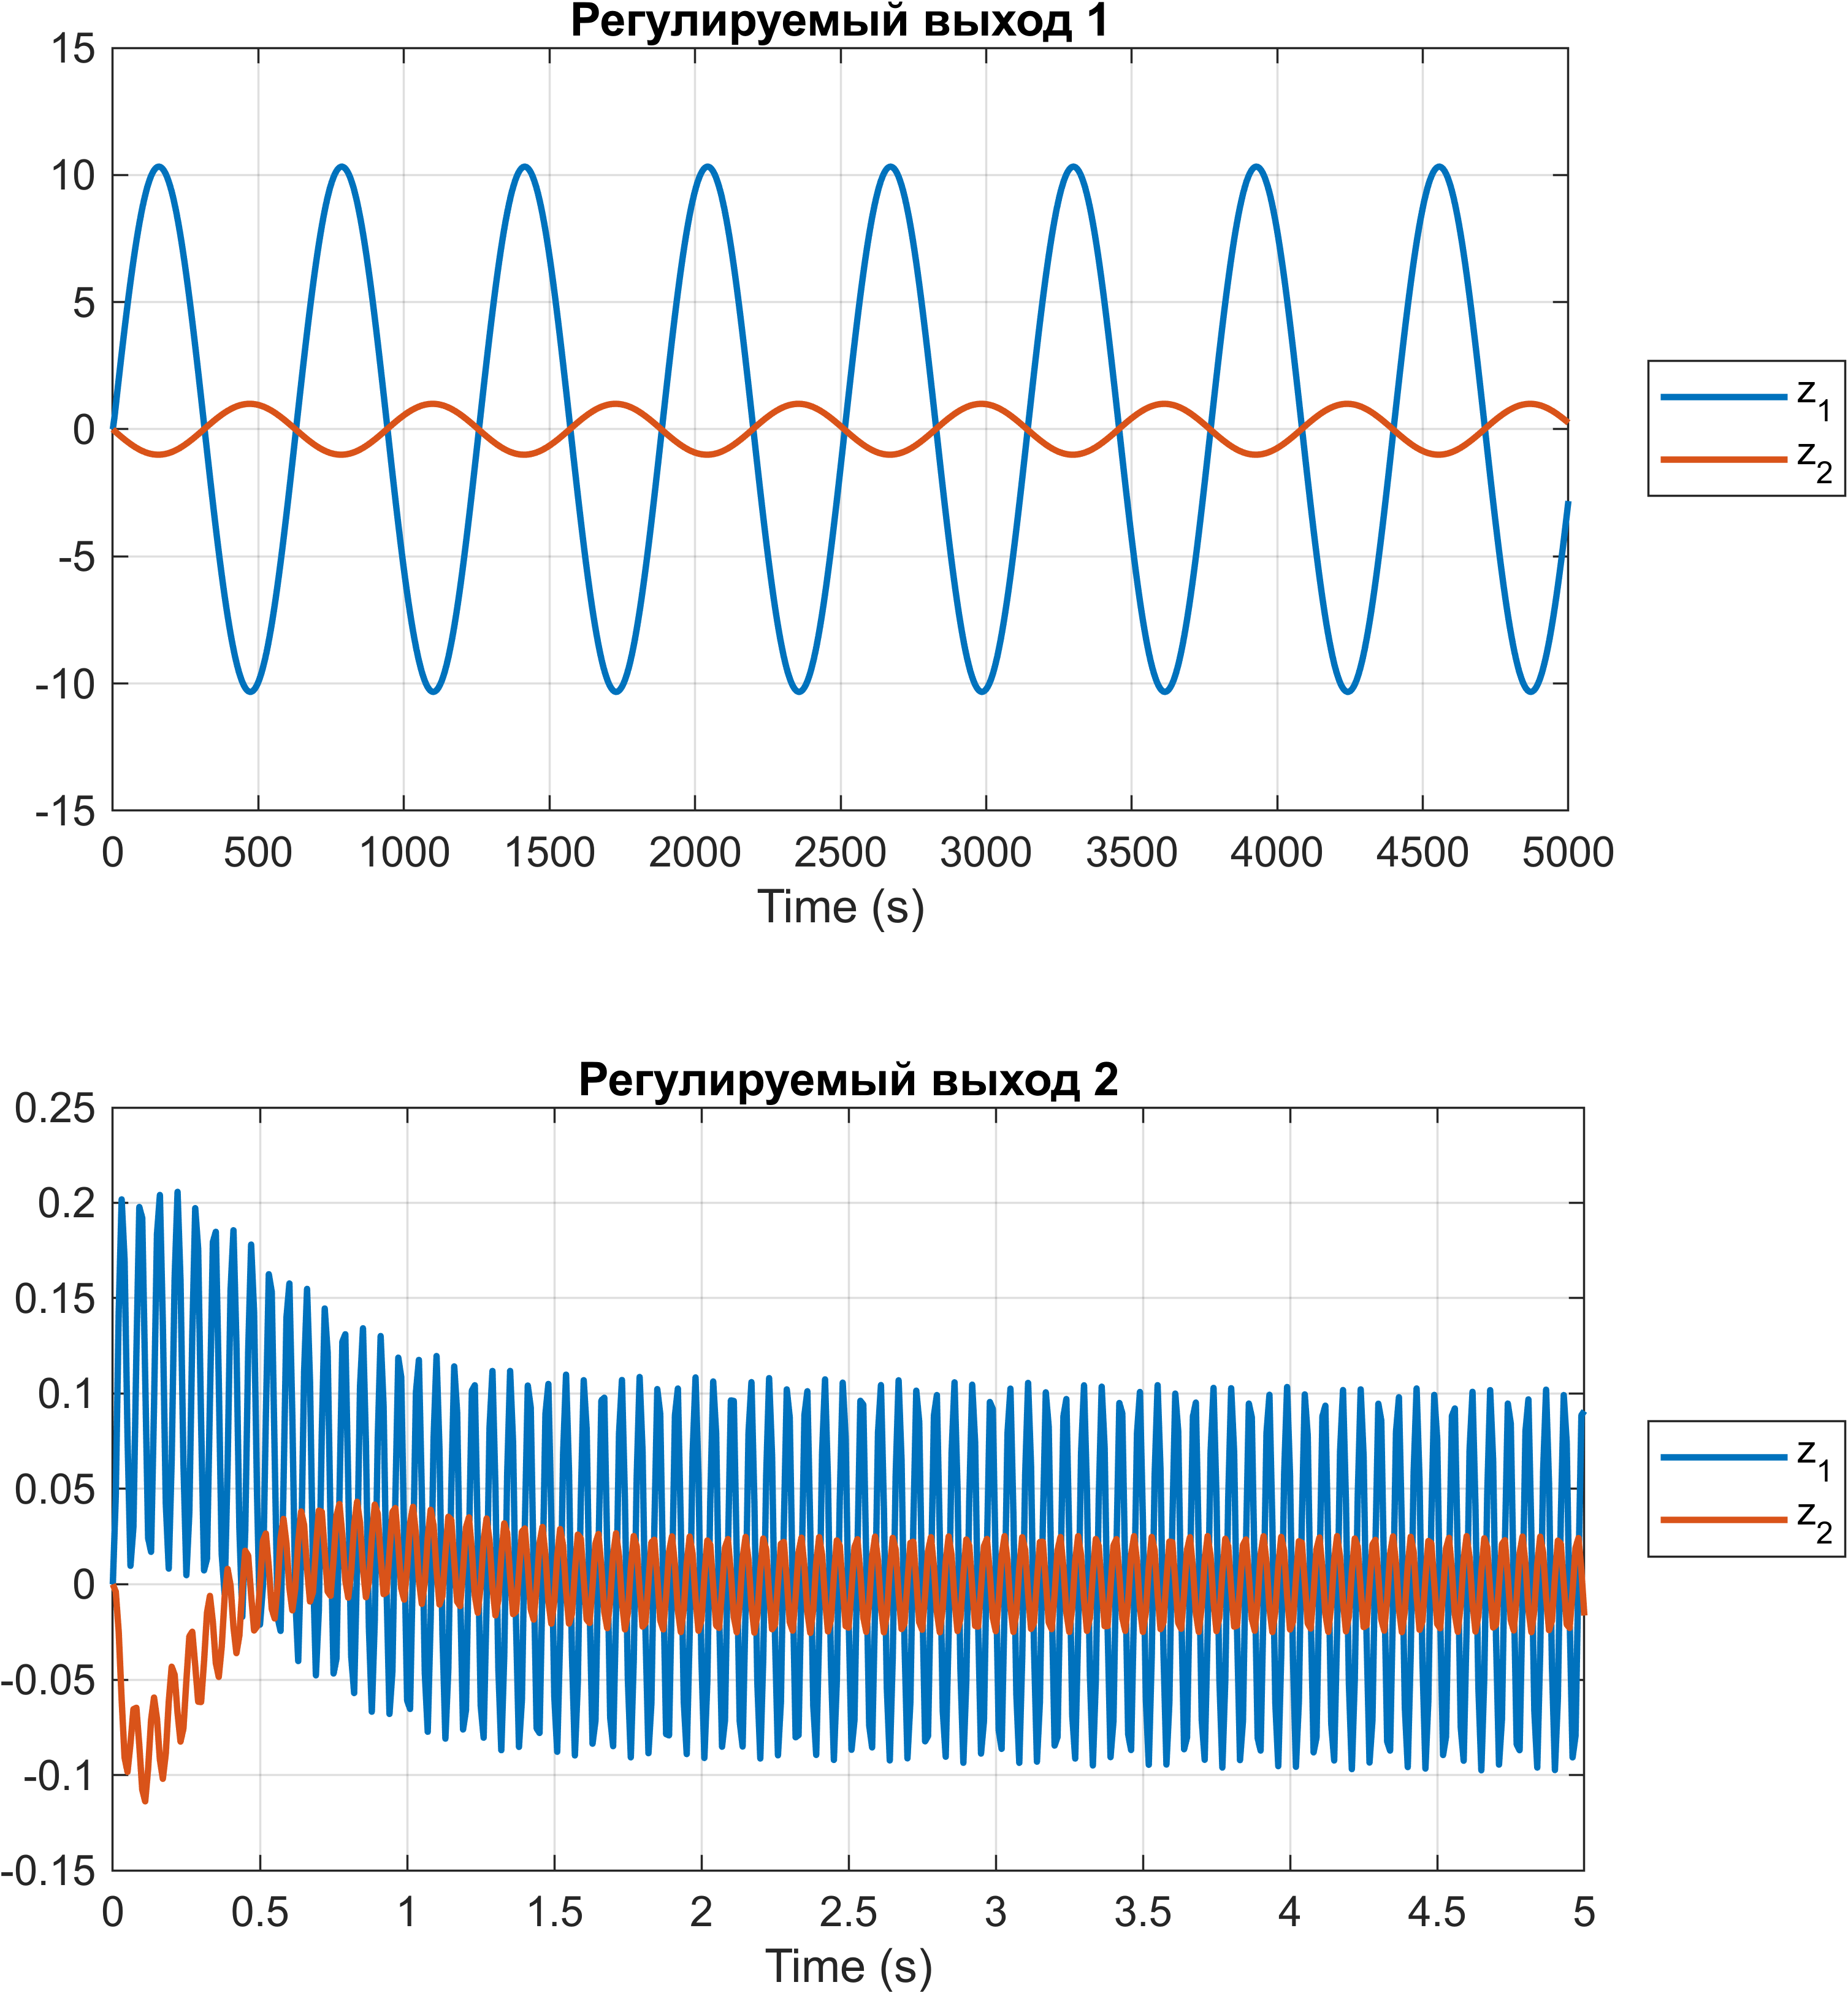
\includegraphics[width=1\linewidth]{figs/7_sim.png}
    \caption{График $z(t)$ при $w_1(t)$ и $w_2(t)$}
    \label{fig:7sim}
\end{figure}

\subsubsection{Выводы}

Из графиков видно, что полностью побороть помеху не удалось, и регулируемый выход 
колеблется около нуля, что естественно, так как нашей задачей было минимизировать норму H infinity. 
Также видно, что на частоте 0.01 амплитуда колебаний на порядок больше чем при частоте 100,
это из-за того, что какого либо большого пика на графике сингулярных чисел и не было, и регулятору не много с чем было работать (но выпрямление графика сингулярных числе все равно видно), 
если сравнить нормы H infinity по выходу и H2-регулятора
по выходу, то видно, что H infinity норма уменьшилась, на графике регулируемого выхода тоже видно,
что в наихудшем случае упала амплитуда колебаний, так что можно сделать вывод, что регулятор
работает.


\subsection{Гамма побольше}

Аналогично синтезируем H infinity регулятор, но уже для значительно большего $\gamma=1000$.
Используя \texttt{icare} получим
\begin{equation*}
    K=\begin{bmatrix}
        -10.0001	&-4.4722
    \end{bmatrix}.
\end{equation*}
Найдем $L$ через решение уравнения \eqref{eq:ric4}, используя \texttt{icare} получим
\begin{equation*}
    L=\begin{bmatrix}
        -1.7323&
        -1.0002
    \end{bmatrix}^T.
\end{equation*}
Передаточная матрица замкнутой системы от внешнего возмущения $w$ к выходу $z$:
\begin{equation*}
    \underset{w\rightarrow z}{W}(s)=\begin{bmatrix}
        \underset{w\rightarrow z}{W_1}(s) & \underset{w\rightarrow z}{W_2}(s)\\
        \underset{w\rightarrow z}{W_3}(s) & \underset{w\rightarrow z}{W_4}(s)
    \end{bmatrix},
\end{equation*}
где
\begin{gather*}
    \underset{w\rightarrow z}{W_1}(s)=\dfrac{10 s^3 + 72.05 s^2 + 249.5 s + 187.5}{s^4 + 6.205 s^3 + 18.75 s^2 + 21.8 s + 10}\\
    \underset{w\rightarrow z}{W_2}(s)=\dfrac{-218 s - 100}{s^4 + 6.205 s^3 + 18.75 s^2 + 21.8 s + 10}\\
    \underset{w\rightarrow z}{W_3}(s)=\dfrac{-21.8 s^2 - 31.8 s - 10}{s^4 + 6.205 s^3 + 18.75 s^2 + 21.8 s + 10}\\
    \underset{w\rightarrow z}{W_4}(s)=\dfrac{-21.8 s^3 - 10 s^2 + 1.041e-15 s + 4.779e-16}{s^4 + 6.205 s^3 + 18.75 s^2 + 21.8 s + 10}
\end{gather*}
График покомпонентных АЧХ $\underset{w\rightarrow z}{W}(s)$ представлен на \autoref{fig:8bodemag}.
\begin{figure}[H]
    \centering
    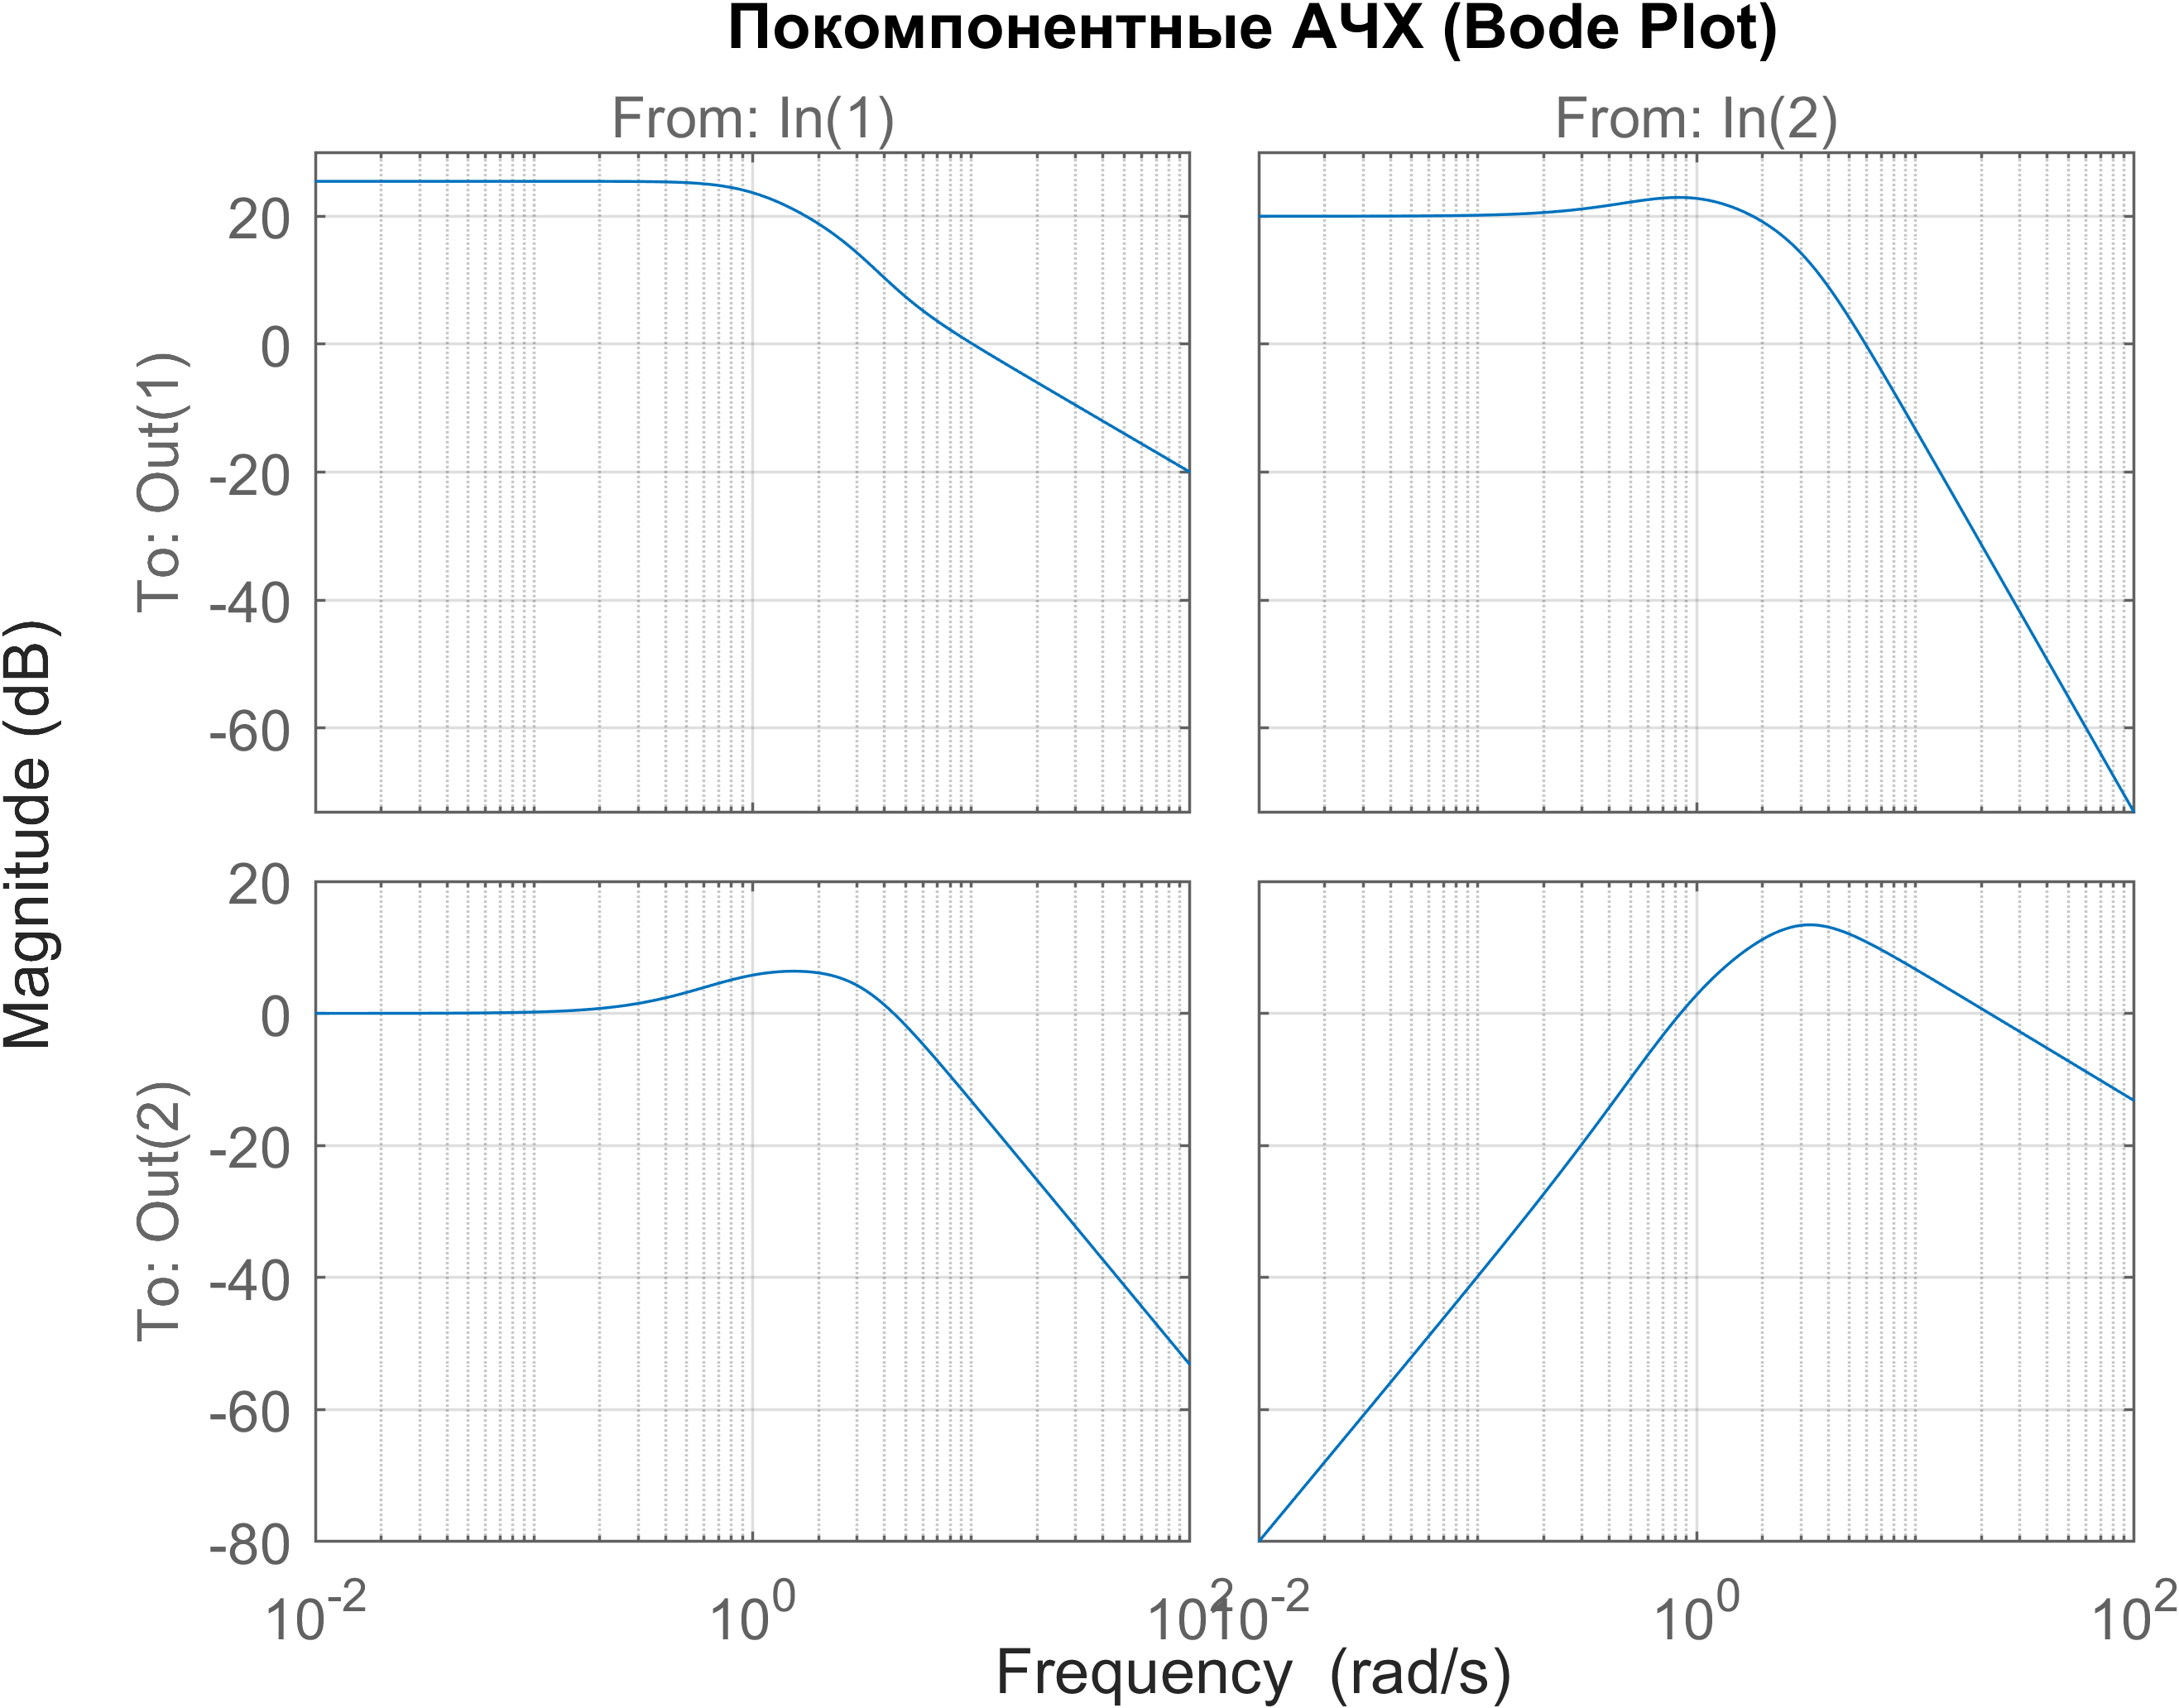
\includegraphics[width=0.8\linewidth]{figs/8_bodemag.png}
    \caption{Покомпонентные АЧХ $\underset{w\rightarrow z}{W}(s)$}
    \label{fig:8bodemag}
\end{figure}
График сингулярных чисел $\underset{w\rightarrow z}{W}(s)$ представлен на \autoref{fig:8sigma}.
\begin{figure}[H]
    \centering
    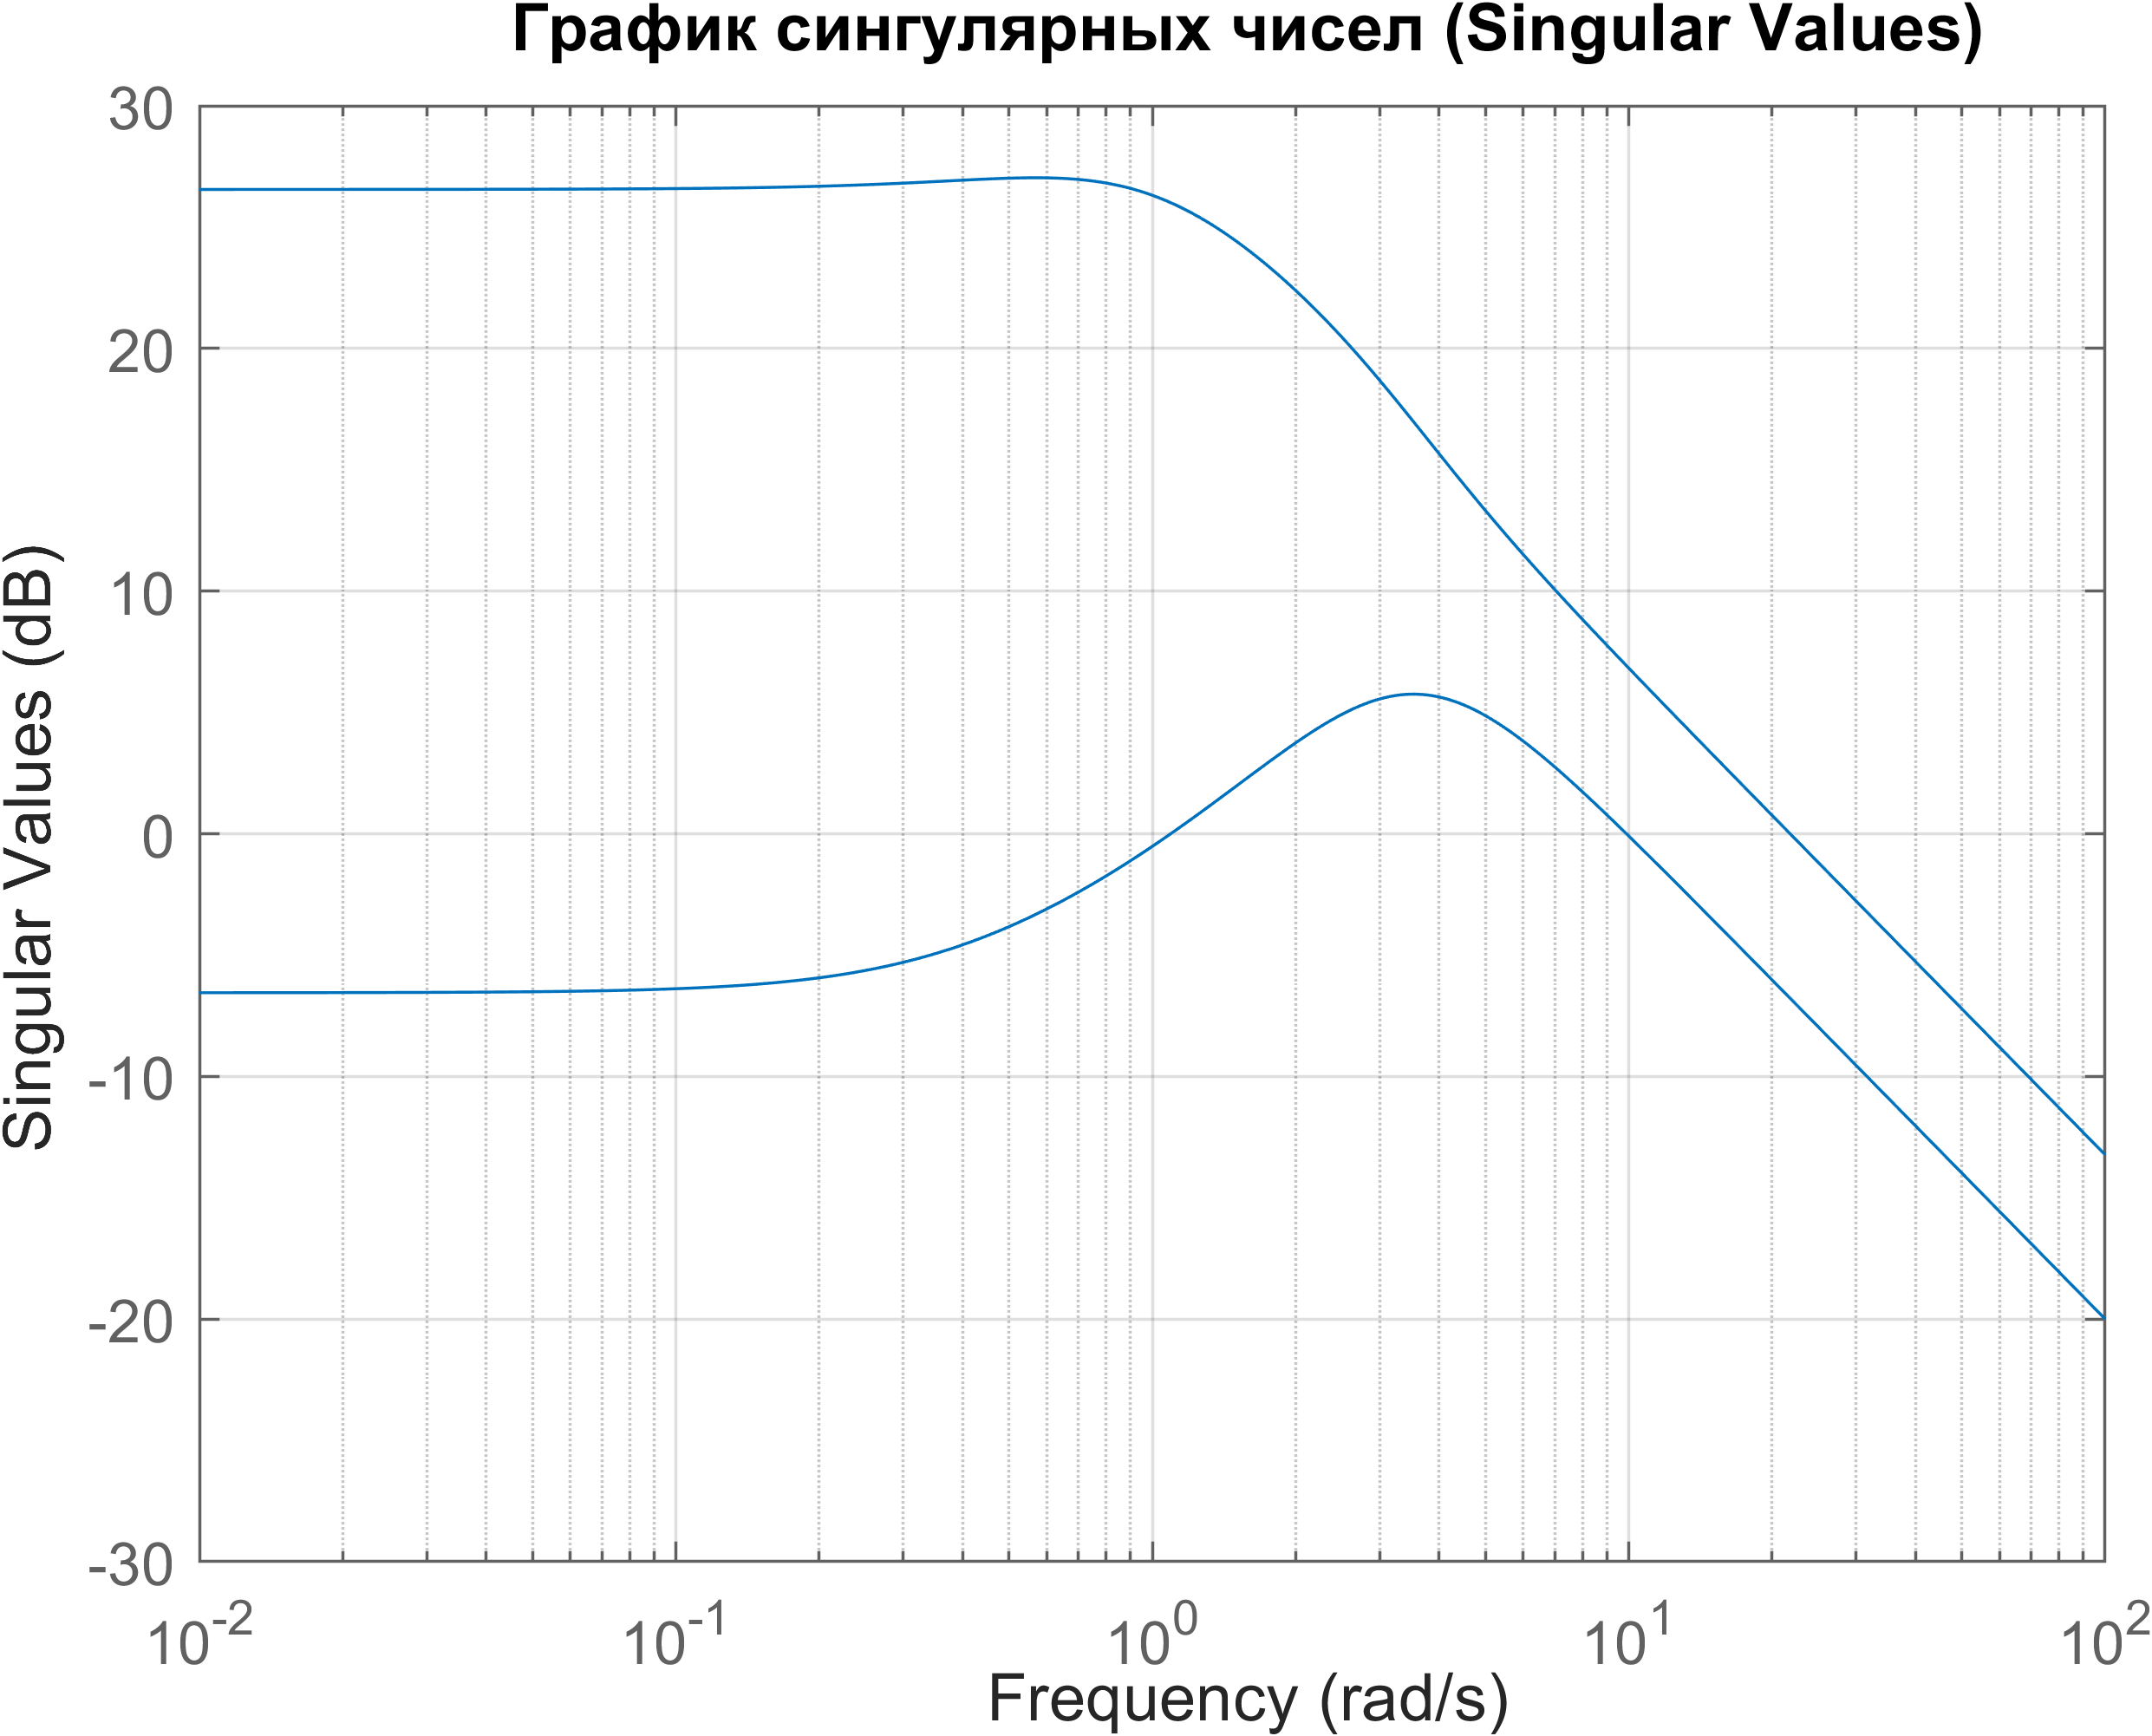
\includegraphics[width=0.8\linewidth]{figs/8_sigma.png}
    \caption{Сингулярные числа $\underset{w\rightarrow z}{W}(s)$}
    \label{fig:8sigma}
\end{figure}
\noindent Найдем нормы $\underset{w\rightarrow z}{W}(s)$:
\begin{equation*}
    ||\underset{w\rightarrow z}{W}(s)||_{H2}=18.6140,\quad
    ||\underset{w\rightarrow z}{W}(s)||_{H\infty}=22.4746.
\end{equation*}
Как видно из графика сингулярных числе, наихудшая частота возмущения $1$.
Таким образом, зададимся двумя возмущениями:
\begin{equation*}
    w_1(t)=\begin{bmatrix}
        sin(t)\\
        0
    \end{bmatrix},\quad
    w_2(t)=\begin{bmatrix}
        sin(100t)\\
        0
    \end{bmatrix}.
\end{equation*}
С помощью SIMULINK (см. \autoref{fig:3slx}) для каждого из выбранных вариантов внешнего возмущения $w$ выполним 
компьютерное моделирование замкнутой системы при нулевых начальных условиях
на объекте управления и построим графики компонент регулируемого выхода
$z(t)$, которые можно увидеть на \autoref{fig:8sim}.
\begin{figure}[H]
    \centering
    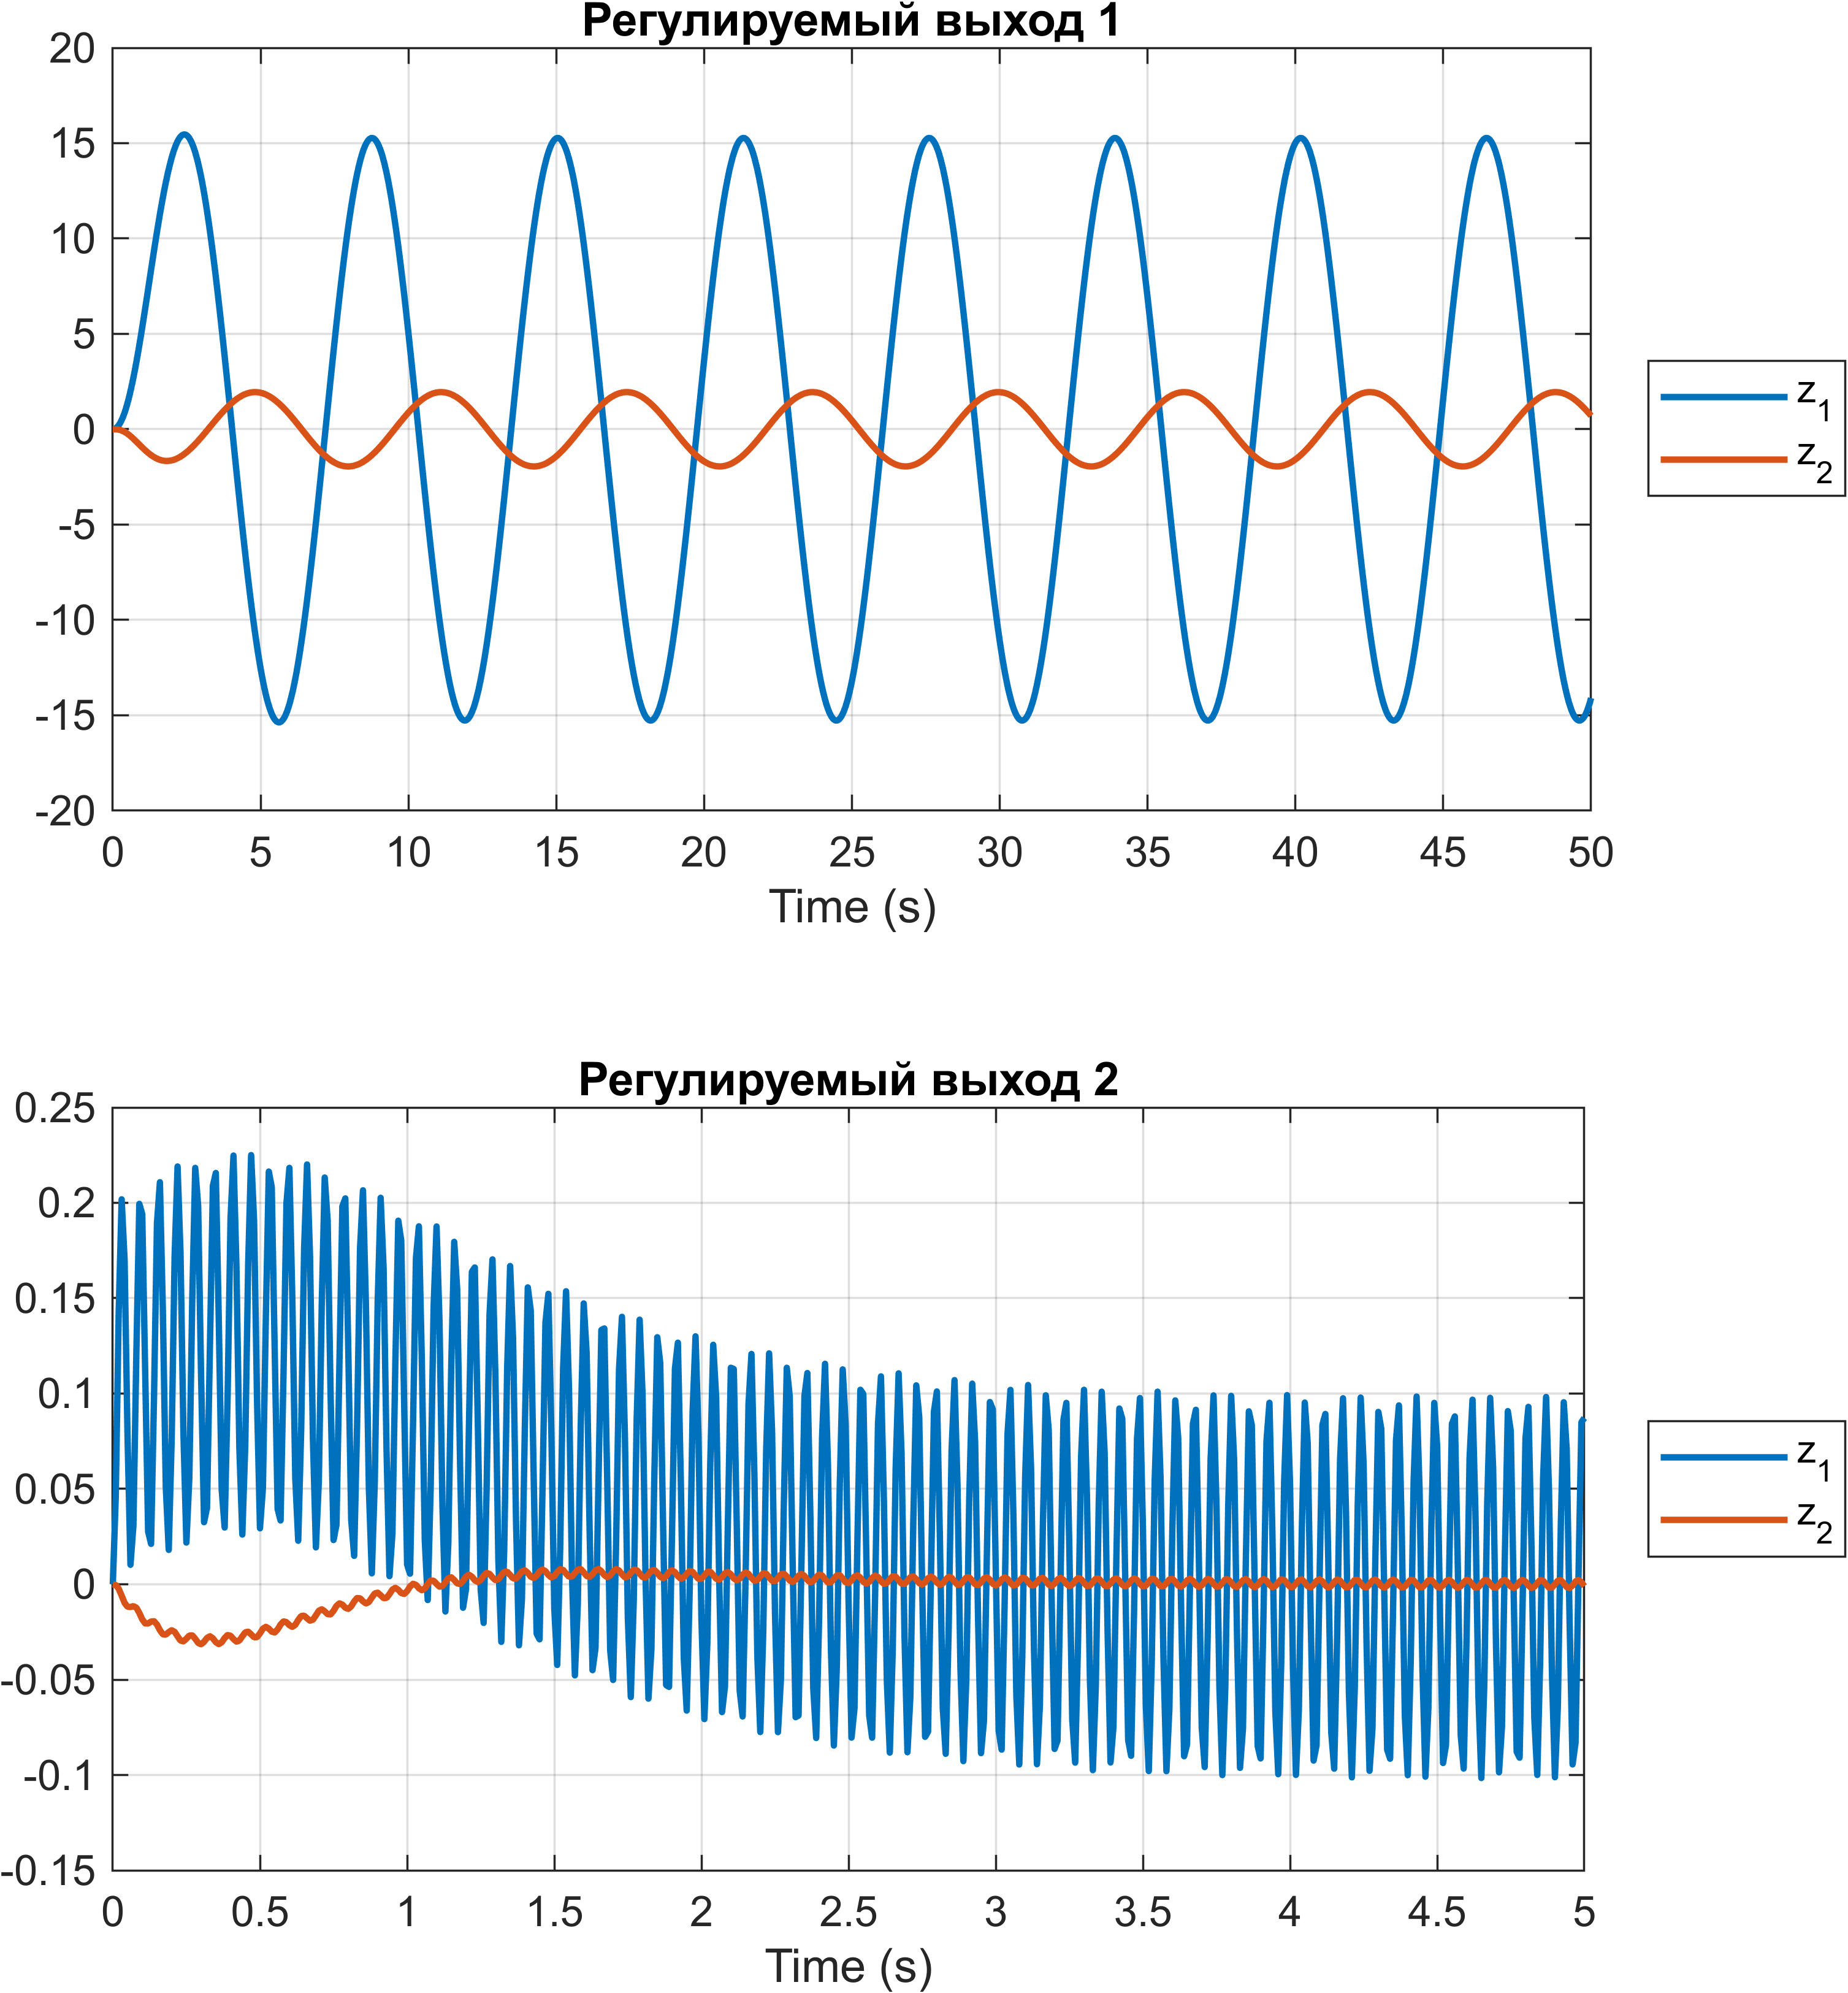
\includegraphics[width=1\linewidth]{figs/8_sim.png}
    \caption{График $z(t)$ при $w_1(t)$ и $w_2(t)$}
    \label{fig:8sim}
\end{figure}

\subsubsection{Выводы}

Из графиков видно, что полностью побороть помеху не удалось, и регулируемый выход 
колеблется около нуля, что естественно, так как нашей задачей было минимизировать норму H infinity. 
Но также видно, что на частоте 1 амплитуда колебаний в несколько раз больше чем при частоте 100,
что напоминает график выхода H2-регулятора \autoref{fig:4sim}.
Можно сделать вывод, что при большой гамме H infinity регулятор становится H2-регулятором.



\section{Заключение}
В ходе лабораторной работы были синтезированы $\mathcal{H}_2$- и $\mathcal{H}_\infty$-регуляторы 
по состоянию и по выходу для двух вариантов регулируемого выхода. 
Проведено моделирование замкнутых систем, построены графики АЧХ, 
сингулярных чисел и передаточных матриц. Регуляторын успечно работали и минимизировали соответствующие нормы. 
Было установлено, что $\mathcal{H}_\infty$-регуляторы 
эффективно минимизируют норму $\mathcal{H}_\infty$ при минимальных $\gamma$, но 
при больших значениях $\gamma$ становятся 
аналогичны $\mathcal{H}_2$-регуляторам.